\documentclass[
  jou,
  floatsintext,
  longtable,
  nolmodern,
  notxfonts,
  notimes,
  donotrepeattitle,
  colorlinks=true,linkcolor=blue,citecolor=blue,urlcolor=blue]{apa7}

\usepackage{amsmath}
\usepackage{amssymb}



\usepackage[bidi=default]{babel}
\babelprovide[main,import]{english}


\babelfont{rm}[,RawFeature={fallback=mainfontfallback}]{Times New Roman}
% get rid of language-specific shorthands (see #6817):
\let\LanguageShortHands\languageshorthands
\def\languageshorthands#1{}

\RequirePackage{longtable}
\RequirePackage{threeparttablex}

\makeatletter
\renewcommand{\paragraph}{\@startsection{paragraph}{4}{\parindent}%
	{0\baselineskip \@plus 0.2ex \@minus 0.2ex}%
	{-.5em}%
	{\normalfont\normalsize\bfseries\typesectitle}}

\renewcommand{\subparagraph}[1]{\@startsection{subparagraph}{5}{0.5em}%
	{0\baselineskip \@plus 0.2ex \@minus 0.2ex}%
	{-\z@\relax}%
	{\normalfont\normalsize\bfseries\itshape\hspace{\parindent}{#1}\textit{\addperi}}{\relax}}
\makeatother




\usepackage{longtable, booktabs, multirow, multicol, colortbl, hhline, caption, array, float, xpatch}
\setcounter{topnumber}{2}
\setcounter{bottomnumber}{2}
\setcounter{totalnumber}{4}
\renewcommand{\topfraction}{0.85}
\renewcommand{\bottomfraction}{0.85}
\renewcommand{\textfraction}{0.15}
\renewcommand{\floatpagefraction}{0.7}

\usepackage{tcolorbox}
\tcbuselibrary{listings,theorems, breakable, skins}
\usepackage{fontawesome5}

\definecolor{quarto-callout-color}{HTML}{909090}
\definecolor{quarto-callout-note-color}{HTML}{0758E5}
\definecolor{quarto-callout-important-color}{HTML}{CC1914}
\definecolor{quarto-callout-warning-color}{HTML}{EB9113}
\definecolor{quarto-callout-tip-color}{HTML}{00A047}
\definecolor{quarto-callout-caution-color}{HTML}{FC5300}
\definecolor{quarto-callout-color-frame}{HTML}{ACACAC}
\definecolor{quarto-callout-note-color-frame}{HTML}{4582EC}
\definecolor{quarto-callout-important-color-frame}{HTML}{D9534F}
\definecolor{quarto-callout-warning-color-frame}{HTML}{F0AD4E}
\definecolor{quarto-callout-tip-color-frame}{HTML}{02B875}
\definecolor{quarto-callout-caution-color-frame}{HTML}{FD7E14}

%\newlength\Oldarrayrulewidth
%\newlength\Oldtabcolsep


\usepackage{hyperref}




\providecommand{\tightlist}{%
  \setlength{\itemsep}{0pt}\setlength{\parskip}{0pt}}
\usepackage{longtable,booktabs,array}
\usepackage{calc} % for calculating minipage widths
% Correct order of tables after \paragraph or \subparagraph
\usepackage{etoolbox}
\makeatletter
\patchcmd\longtable{\par}{\if@noskipsec\mbox{}\fi\par}{}{}
\makeatother
% Allow footnotes in longtable head/foot
\IfFileExists{footnotehyper.sty}{\usepackage{footnotehyper}}{\usepackage{footnote}}
\makesavenoteenv{longtable}

\usepackage{graphicx}
\makeatletter
\newsavebox\pandoc@box
\newcommand*\pandocbounded[1]{% scales image to fit in text height/width
  \sbox\pandoc@box{#1}%
  \Gscale@div\@tempa{\textheight}{\dimexpr\ht\pandoc@box+\dp\pandoc@box\relax}%
  \Gscale@div\@tempb{\linewidth}{\wd\pandoc@box}%
  \ifdim\@tempb\p@<\@tempa\p@\let\@tempa\@tempb\fi% select the smaller of both
  \ifdim\@tempa\p@<\p@\scalebox{\@tempa}{\usebox\pandoc@box}%
  \else\usebox{\pandoc@box}%
  \fi%
}
% Set default figure placement to htbp
\def\fps@figure{htbp}
\makeatother


% definitions for citeproc citations
\NewDocumentCommand\citeproctext{}{}
\NewDocumentCommand\citeproc{mm}{%
  \begingroup\def\citeproctext{#2}\cite{#1}\endgroup}
\makeatletter
 % allow citations to break across lines
 \let\@cite@ofmt\@firstofone
 % avoid brackets around text for \cite:
 \def\@biblabel#1{}
 \def\@cite#1#2{{#1\if@tempswa , #2\fi}}
\makeatother
\newlength{\cslhangindent}
\setlength{\cslhangindent}{1.5em}
\newlength{\csllabelwidth}
\setlength{\csllabelwidth}{3em}
\newenvironment{CSLReferences}[2] % #1 hanging-indent, #2 entry-spacing
 {\begin{list}{}{%
  \setlength{\itemindent}{0pt}
  \setlength{\leftmargin}{0pt}
  \setlength{\parsep}{0pt}
  % turn on hanging indent if param 1 is 1
  \ifodd #1
   \setlength{\leftmargin}{\cslhangindent}
   \setlength{\itemindent}{-1\cslhangindent}
  \fi
  % set entry spacing
  \setlength{\itemsep}{#2\baselineskip}}}
 {\end{list}}
\usepackage{calc}
\newcommand{\CSLBlock}[1]{\hfill\break\parbox[t]{\linewidth}{\strut\ignorespaces#1\strut}}
\newcommand{\CSLLeftMargin}[1]{\parbox[t]{\csllabelwidth}{\strut#1\strut}}
\newcommand{\CSLRightInline}[1]{\parbox[t]{\linewidth - \csllabelwidth}{\strut#1\strut}}
\newcommand{\CSLIndent}[1]{\hspace{\cslhangindent}#1}





\usepackage{fontspec} 

\defaultfontfeatures{Scale=MatchLowercase}
\defaultfontfeatures[\rmfamily]{Ligatures=TeX,Scale=1}

  \setmainfont[,RawFeature={fallback=mainfontfallback}]{Times New Roman}




\title{Probing the Limits of Memory: Can A Learned Response Persist
Through Decapitation and Regeneration in Planaria?}


\shorttitle{Persistance of Memory Through Regeneration in Planaria}


\usepackage{etoolbox}






\author{Francis Charles Forde}



\affiliation{
{School of Psychology, Victoria University of Wellington}}




\leftheader{Forde}



\abstract{Although researchers have made immense progress in
understanding how memories are formed and stored, research stemming from
the invertebrate literature is forcing us to question some of our
assumptions about the nature of memory. Using planaria, a flatworm with
a centralised brain and incredible regenerative capabilities,
researchers have shown that simple associative memories can be retained
in the brainless tail halves after decapitation. But these basic
eperiments leave important questions unanswered. For example, are
complex memories necessarily stored in networks of neurons and their
synaptic weights? Or can they too be stored in tissues outside of the
central nervous system? To answer this question, we performed a series
of Experiments to determine whether planaria can acquire and retain an
operantly conditioned response for at least two weeks, and whether this
can be retained in the brainless tail halves of decapitated planaria. In
the experiments reported here, we first established baseline preferences
for subjects to determine their arm preference in a Y-shaped maze.
During conditioning, treatment subjects were rewarded with either
cocaine or methamphetamine for entering the least prefered arm, while
control subjects received vehicle only (distilled water) for doing so.
In the key experiments performed here, subjects were then bisected into
head and tail halves and left to regenerate. 14 days later, the head and
tail halves were tested for retention of the conditioned response. The
next day, subjects were exposed to the rewarding compound to identify
whether the memory could be brought back with a reinstatement procedure.
Overall, the results were inconclusive as to whether planaria can learn
and retain a conditioned response through decapitation and regeneration.
While experiments 3 and 4 provided preliminary evidence for learning
compared to control subjects, experiment 2 and 5 failed to show a
signficant change in behaviour compared to control subjects. Regarding
retention, we failed to find evidence that the learned response can be
retained.However, given the extent of learning was relatively weak,
future experiments will be required to improve on the training procedure
used here or to find a suitable alternative method for shaping complex
behaviours among planaria. Only then will it be possible to test whether
complex memories can survive through decapitation and regeneration.
Although the literature insists that planaria are useful for answering
questions relating to addiction and other learning processes, more
sophisticated learning tasks must be established if we are to produce
insights relating to the kinds of memories we care about.}

\keywords{Memory, Learning, Planaria, Reinstatement, Cocaine, Methamphetamine, Behaviour}

\authornote{ 

\par{   The author has no conflicts of interest to disclose. This Thesis
was supported by a Wellington Masters by Thesis Scholarship provided by
Victoria University of Wellington. Thanks is owed to . . .  }
\par{Correspondence concerning this article should be addressed to }
}

\usepackage{pbalance} 
\usepackage{float}
\makeatletter
\let\oldtpt\ThreePartTable
\let\endoldtpt\endThreePartTable
\def\ThreePartTable{\@ifnextchar[\ThreePartTable@i \ThreePartTable@ii}
\def\ThreePartTable@i[#1]{\begin{figure}[!htbp]
\onecolumn
\begin{minipage}{0.5\textwidth}
\oldtpt[#1]
}
\def\ThreePartTable@ii{\begin{figure}[!htbp]
\onecolumn
\begin{minipage}{0.5\textwidth}
\oldtpt
}
\def\endThreePartTable{
\endoldtpt
\end{minipage}
\twocolumn
\end{figure}}
\makeatother


\makeatletter
\let\endoldlt\endlongtable		
\def\endlongtable{
\hline
\endoldlt}
\makeatother

\newenvironment{twocolumntable}% environment name
{% begin code
\begin{table*}[!htbp]%
\onecolumn%
}%
{%
\twocolumn%
\end{table*}%
}% end code

\urlstyle{same}



\makeatletter
\@ifpackageloaded{caption}{}{\usepackage{caption}}
\AtBeginDocument{%
\ifdefined\contentsname
  \renewcommand*\contentsname{Table of contents}
\else
  \newcommand\contentsname{Table of contents}
\fi
\ifdefined\listfigurename
  \renewcommand*\listfigurename{List of Figures}
\else
  \newcommand\listfigurename{List of Figures}
\fi
\ifdefined\listtablename
  \renewcommand*\listtablename{List of Tables}
\else
  \newcommand\listtablename{List of Tables}
\fi
\ifdefined\figurename
  \renewcommand*\figurename{Figure}
\else
  \newcommand\figurename{Figure}
\fi
\ifdefined\tablename
  \renewcommand*\tablename{Table}
\else
  \newcommand\tablename{Table}
\fi
}
\@ifpackageloaded{float}{}{\usepackage{float}}
\floatstyle{ruled}
\@ifundefined{c@chapter}{\newfloat{codelisting}{h}{lop}}{\newfloat{codelisting}{h}{lop}[chapter]}
\floatname{codelisting}{Listing}
\newcommand*\listoflistings{\listof{codelisting}{List of Listings}}
\makeatother
\makeatletter
\makeatother
\makeatletter
\@ifpackageloaded{caption}{}{\usepackage{caption}}
\@ifpackageloaded{subcaption}{}{\usepackage{subcaption}}
\makeatother
\makeatletter
\@ifpackageloaded{sidenotes}{}{\usepackage{sidenotes}}
\@ifpackageloaded{marginnote}{}{\usepackage{marginnote}}
\makeatother

% From https://tex.stackexchange.com/a/645996/211326
%%% apa7 doesn't want to add appendix section titles in the toc
%%% let's make it do it
\makeatletter
\xpatchcmd{\appendix}
  {\par}
  {\addcontentsline{toc}{section}{\@currentlabelname}\par}
  {}{}
\makeatother

\begin{document}

\maketitle

\hypertarget{toc}{}
\tableofcontents
\newpage
\section[Introduction]{Probing the Limits of Memory: Can A Learned
Response Persist Through Decapitation and Regeneration in Planaria?}

\setcounter{secnumdepth}{5}

\setlength\LTleft{0pt}


\section*{Acknowledgements}\label{acknowledgements}
\addcontentsline{toc}{section}{Acknowledgements}

Thanks is owed to my supervisors, Dr.~{[}Name{]} and

\newpage

\phantomsection\label{toc}
\section*{Table of Contents}\label{table-of-contents}
\addcontentsline{toc}{section}{Table of Contents}

\newpage

\section{Introduction}\label{sec-introduction}

A brain in isolation is just a clump of extravagant cells. A brain earns
its keep by liaising with the body and the external world. It is among
these brain-environment interactions that an organism can set and
achieve goals and, ultimately, carve a pathway to survival. But brains
operate in the dark. Their only insight into the on-goings of the world
is through delicately placed sensory organs such as the eyes, nose and
ears.

The sensory technology that each organism possesses, what philosophers
call its sensorium, differs across species. Some build a picture of the
world by capturing light using light sensitive proteins. Others live
where no light can penetrate and so must form their worldview using
other sensory modalities like echolocation. Notwithstanding these
differences, neuroscientists and biologists seek to understand the suite
of abilities each organism possesses, the neuronal and molecular
mechanisms which underpin these, and the factors that determine when and
why an organism deploys the behaviours in its arsenal. But we do not
usually do this for the sake of the organism itself. Rather, we use
non-human organisms with the hope of learning something about our own
brains and bodies.

We now have a broad tool set for inspecting brains across different time
spans and at different levels of analysis. From looking at activity
within a single dendritic spine over microseconds to looking at
connectivity between different brain structures over several minutes. We
can even track changes in the size of spines on a single dendrite over
time -- impressive given the width of a spine is 100 times smaller than
the thickness of a human hair
(\citeproc{ref-bayramoglu_hair_2022}{Bayramoglu et al., 2022};
\citeproc{ref-li_current_2023}{B.-Z. Li et al., 2023}). At the network
level, we are able to identify groups of neurons (ensembles) involved in
encoding and storing memory, and can use precise tools to excite or
inhibit those networks to alter an animals behaviour
(\citeproc{ref-goshen_optogenetic_2014}{Goshen, 2014}).

Our experimental competency arose from many small steps. Before we had
the capability for manipulating neurons to understand their role in
memory, we had to attack things more abstractly. Our early exploration
of how memory functions involved basic procedures like learning lists of
nonsense syllables or simple motor tasks. This early research helped
answer the question of whether memory is a unitary system or a suite of
separate systems which can be dissociated. Out of this fell distinctions
between episodic and semantic memory, as well as short- and long-term
memory storage. Early theoretical progress provided the foundation upon
which specialised tools and procedures could be developed to manipulate
and characterise the biology of memory in its different forms.

\subsection{Overview of Key Concepts in the Field of Learning and
Memory}\label{overview-of-key-concepts-in-the-field-of-learning-and-memory}

\subsubsection{Categories of Memory}\label{categories-of-memory}

Memory is the embodiment of past experience which shapes our future
behaviour. Learning, on the other hand, is the process of memory
acquisition. That said, there may be as many different definitions of
learning and memory as there are papers published on the topic. Barron
et al. (\citeproc{ref-barron_embracing_2015}{2015}) surveyed the various
uses of the term ``learning'' across disciplines such as cognitive
psychology, behavioural ecology, and machine learning and identified at
least 50 definitions (albeit with a lot of overlap). Memory has been
parceled into several distinct categories based on the content of the
information held (see Figure~\ref{fig-figure1} below). A major
distinction was made between explicit and implicit memory
(\citeproc{ref-schacter_memory_1994}{Schacter \& Tulving, 1994};
\citeproc{ref-squire_memory_1987}{Squire, 1987}). Explicit memories are
those accessible to conscious awareness, like a memory of where you
parked your car this morning. Implicit memories cannot be consciously
accessed but still affect behaviour, an example being the small muscle
movements needed to ride a bike. Explicit memory has been further
subdivided into episodic and semantic memory
(\citeproc{ref-tulving_episodic_1972}{Tulving, 1972}). Episodic refers
to the rich experiential quality of personal memories, while semantic
relates to things that you know but which lack an experiential
component, such as facts about the world.

Memory can also be categorised temporally. Atkinson and Shiffrin
(\citeproc{ref-spence_human_1968}{1968}) proposed a model with three
stores that process memories over time: a sensory register, short-term
store, and long-term store. This division is still usefully applied in
the field of learning and memory (e.g.,
\citeproc{ref-miller_timescales_2024}{Miller \& Constantinidis, 2024}).
The temporal framing of memory reflects the process of learning itself.
Learning is normally broken up into several stages, each building on
prior stages to fortify the memory and increase its longevity (see
Section~\ref{sec-mechanisms} below). Initially, information we process
enters a short-term state and may alter behaviour and decision making in
the immediate future. However, most sensory information is not retained.
Only meaningful information is given permanent residence. For this to
occur, a set of active processes are required to ensure the information
is maintained so that it can be accessed in perpetuity. This stage,
known as consolidation, pushes back against the otherwise imminent
process of forgetting.

These distinctions are reasonable in the context of human memory. But it
is not clear whether these distinctions generalise to other organisms.
Most people do not attribute rich experiential memories to rodents, let
alone invertebrates. Yet even very simple organisms such as planaria
(see Section~\ref{sec-planaria-as-a-model-organism}) have the capacity
to retain and act on information from their environment. Viewing memory
as a range of dissociable information stores is particularly relevant
when investigating whether information can be stored outside of the
central nervous system. If, as recent research suggests
(\citeproc{ref-shomrat_automated_2013}{Shomrat \& Levin, 2013}),
memories are able to be stored outside the brain, the categories
outlined here will help us to explore which forms of information have
this property and which do not.

While non-associative memories such as sensitisation may be stored
outside of neural networks, perhaps rich episodic experiences can only
be stored among complex ensembles of neurons in the brain. We do not yet
know the bounds memory storage outside of the central nervous system.
Armed with these conceptual distinctions of memory, researchers can
investigate a broad range of training techniques to identify which forms
of memory persist outside the brain and which do not.

\begin{figure}[!htbp]

{\caption{{Categorisation of Memory}{\label{fig-figure1}}}}

\begin{center}
\pandocbounded{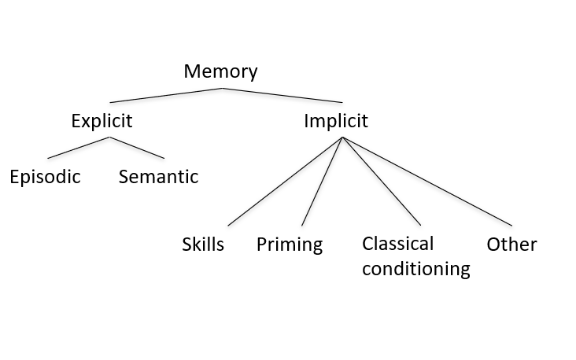
\includegraphics[keepaspectratio]{Francis_Masters_Thesis_files/figure-pdf/fig-figure1-1.png}}
\end{center}

{\noindent \emph{Note.} Theoretical categorisation of memory based on
the content and conscious accessibility of the information. The major
explicit/implicit distinction was first put forward by Endel Tulving
(1972). Figure adapted from Squire (1987).}

\end{figure}

\subsubsection{Associative and Non-associative
Learning}\label{associative-and-non-associative-learning}

Associative learning requires learning the temporal relationship between
two stimuli. For example, one stimulus reliably precedes another, or a
behaviour reliably elicits a reward. Non-associative forms of learning
captures learning about a stimulus itself, but not in relation to other
stimuli. This typically takes the form of behavioural sensitisation or
habituation. If you were to deliver a mild shock to my hand, I would
withdraw it reflexively as part of the innate startle response. But with
repeated administration of the shock over time, I would learn that the
shock is not harmful. The size of my startle response would decrease
(habituation). I have learned something about the shock, but have
learned nothing about its temporal relationship with other stimuli. To
translate this example to an associative form of learning, a moderate
shock could be delivered after being shown a picture of a sunflower. I
would learn an association between the flower imagery and the subsequent
painful experience. With repeated pairings, I would display a preemptive
startle response (tense muscles, squint my eyes, dip my head) to
presentations of the flower alone. I have learnt a temporal association
between the flower and the shock such that my body now predicts and
prepares for the shock before it arrives.

Classical conditioning and operant conditioning are two frequently used
forms of associative learning. Classical conditioning involves learning
an association between two or more stimuli, as in the flower/shock
example above. Operant conditioning differs from classical conditioning
in that rather than one stimulus being paired with another stimulus, a
behaviour comes to be associated with a specific outcome. For example, I
learn that signing up to psychology experiments often involves being
exposed to irritating stimuli. This changes the likelihood of that
response being produced in the future. In other words, I stop signing up
as a participant.

\subsubsection{Maladaptive Learning}\label{maladaptive-learning}

The examples outline above capture learning in cases where it is
beneficial for the learner. In the classical conditioning case described
above, preparing for a shock by tensing my muscle tissue reduces the
painfulness of the experience and minimises the chance of tissue damage.
For the operant conditioning case, avoiding future experiments would
mean I am exposed to less unnecessary irritants. Although these are
mundane examples, we will all encounter consequential cases whereby our
wellbeing and longevity are enhanced by learning from past experience. A
close call when crossing a road (and the negative physiology experience
that ensues) increases the likelihood of diligently looking both ways
before future crossings. But learning is not always protective.

The capacity for learning leaves us vulnerable to developing maladaptive
habits. Consider Rebecca's first experience with heroine. Prior to
consumption, Rebecca has heard about heroine, but only in the sense that
she knows it is a harmful drug, that similar drugs are used in a medical
setting, and so on. She has no prior subjective experience of its
effects. After several experiences with the drug, she learns about the
intense sense of euphoria that comes from its consumption. Later, Sarah
develops a strong motivation to take the drug again, especially when she
sees drug associated cues (syringes, white powder etc.).

Without the capacity to form such associations, addiction would not be
an issue. Sarah would fail to remember what actions led to such euphoric
experiences, and no motivations would be aroused at the sight of drug
paraphernalia. Addiction arises from the often useful ability to
remember what past actions and events resulted in positive and negative
experiences. In Rebecca's case, the euphoria experienced while initially
using the drug led to a neurological rewiring. It is as if the cognitive
system used for goal pursuit has been hijacked to pursue heroine, even
in the face of adverse consequences
(\citeproc{ref-panksepp_role_2002}{Panksepp et al., 2002};
\citeproc{ref-tan_drugs_2024}{Tan et al., 2024}).

Many aspects of poor mental health, including features of depression,
PTSD, and anxiety, only arise because of our ability to learn. For
example, anxiety entails worry or concern over some perceived threat.
The threat has not yet occurred, but to a person with anxiety, past
experience of similar circumstances creates excessive fear as they
imagine a similar negative outcome occurring in the future. If we can
understand what biological mechanisms create associations between a
context and a negative outcome, as in the case of anxiety, we can then
develop methods which unpick the maladaptive associations and reduce
human suffering. While we have made progress in our understanding of how
memories are forged at the molecular and cellular level, there are many
unknowns which constrain our ability to create useful interventions.

\subsection{Mechanisms of Memory Storage}\label{sec-mechanisms}

As described earlier, the process of acquiring an enduring memory
involves transforming information from a temporary state to a stable
state. But this is not a usual trajectory for most of the information we
encounter. The most common fate is for information to be quickly
forgotten. This is evolutionary sensible. Storing information takes
energy and physical real estate, and attaining energy comes at a price.
Every organism therefore has a small number of things about which it
must study extensively and track over time. But most of the information
an organism encounters, be it visual, tactile, or olfactory, is not
worth storing. A gazelle cares about the scent of a cheetah, but cares
not for the small beetle being crushed under its foot as it moves. While
a gazelle's brain may process information about both stimuli, it is not
equally likely to store both experiences and the contexts in which they
took place.

When discussing how information is stored, one becomes steeped in
complex biological pathways. These pathways involve proteins interacting
with other proteins, proteins interacting with DNA, and the production
of new proteins. In the neurobiological literature, much of the
discussion around learning takes place at the level of the synapse -- a
synapse being the point where two neurons interact. Typically, the axon
from neuron A attaches to a dendrite from neuron B and forms a synapse.
Synapses are the locus of communication in the brain. At an abstract
level, learning occurs when incoming stimulation affects downstream
dendritic spines such that they move through the following sequence of
stages: generation, stabilisation, consolidation, and maintenance (see
\citeproc{ref-rudy_neurobiology_2014}{Rudy, 2014} for a digestible
overview of each stage). Complicated mechanisms are involved in each
stage of learning, and not all the components are fully understood.
Despite that, the literature provides a good account of many important
molecular events thought to be involved in storing information in the
brain so that it can be accessed in the future.

When some new bit of information has been acquired by the brain, its
physical embodiment is referred to as a ``memory trace''
(\citeproc{ref-asok_molecular_2019}{Asok et al., 2019};
\citeproc{ref-robins_21st_2023}{Robins, 2023};
\citeproc{ref-semon_mneme_1921}{Semon, 1921}). To generate this memory
trace, a post-synaptic influx of calcium (resulting from stimulation by
an upstream neuron A) is necessary
(\citeproc{ref-cavazzini_ca2_2005}{Cavazzini et al., 2005};
\citeproc{ref-lynch_intracellular_1983}{Lynch et al., 1983}). Once
inside the pos-synaptic dendrite, calcium interacts with intracellular
proteins that break down actin into smaller chunks
(\citeproc{ref-lynch_ltp_2007}{Lynch et al., 2007}). Although actin
helps give structure to dendritic spines, dissasembly is necessary to
create room for more receptors into the membrane of neuron B. Adding
receptors to the membrane makes the spine on neuron B more sensitive to
the upstream firing of neuron A, and thus more likely to itself fire an
action potential in response. This rapid change in sensitivity
(potentiation) is short lived. Without further processing, the
potentiated state will revert back to baseline.

Stabilisation of the memory trace requires expanding and strengthening
the post-synaptic actin network to solidify the heightened sensitivity
(\citeproc{ref-chen_changes_2007}{Chen et al., 2007}). The spine head is
enlarged and as a result, the actin scaffolding is modified to make it
less vulnerable to being disassembled in the future. In addition to
actin reorganisation, cell adhesion proteins in the cell membrane help
to couple the pre- and post-synaptic neurons, improving the
effectiveness of neurotransmission
(\citeproc{ref-huntley_cadherin_2002}{Huntley et al., 2002}). With these
two key modifications, the pencil marks of memory are laid down. But
these scratchings must be committed to ink to stand the test of time.

Consolidation is where the cellular changes are solidified to stave off
forgetting. Consolidation is unique in that it involves the production
of new proteins. In response to neuronal stimulation, a number of events
take place in the postynaptic neuron. One response is the activation of
proteins which are able to enter the nucleus and bind to DNA. This
activity leads to transcription of new molecules (messenger RNA) that
will later be turned into proteins including receptors. This genomic
signaling ensures new proteins are continually minted, providing a
sufficient pool of receptors and other elements needed to keep the spine
in a state of heightened sensitivity. But the events of consolidation
are not final. The post-synaptic cell enters a maintenance stage where
the supply of membrane receptors produced and inserted into the membrane
remains heightened. Moreover, the typical dynamics of receptor removal
and recycling is slowed. More excitatory receptors remain on the cell
membrane which ensures heightened sensitivity to signals from
presynaptic neurons both now and in the future.

\subsection{Memory Research in Animals and
Invertebrates}\label{memory-research-in-animals-and-invertebrates}

Many organisms have been poked and prodded during our efforts to
understand the mechanisms of memory. Scrub jays, a bird sporting a bold
blue coat and pointed black beak, have been recurring subjects in
studies investigating spatial memory. This is because of their food
caching expertise (\citeproc{ref-shettleworth_how_1982}{Shettleworth \&
Krebs, 1982}). Sophisticated techniques have been used to study changes
in hippocampal volume in response to caching. The possibility of
season-dependent changes in hippocampal neurogenesis in caching birds
has also been explored (reviewed in
\citeproc{ref-pravosudov_25the_2007}{Pravosudov, 2007}).

Rodents have featured heavily in the experimental memory literature
(\citeproc{ref-ghafarimoghadam_review_2022}{Ghafarimoghadam et al.,
2022}). Recent advances in stimulation and imaging, specifically
techniques like optogenetics
(\citeproc{ref-goshen_optogenetic_2014}{Goshen, 2014}) and two-photon
microscopy (\citeproc{ref-kawakami_vivo_2015}{Kawakami et al., 2015}),
have enabled us to study representation of different types of memory at
levels ranging from individual synapses to neuronal ensembles. Moreover,
the last two decades saw a growing interest in episodic memory in
rodents. In the rodent literature, episodic memory is the ability to
represent the past and draw on specific encoded events in a manner akin
to mental time travel (\citeproc{ref-krause_episodic_2022}{Crystal,
2022}; \citeproc{ref-eacott_mental_2007}{Eacott \& Easton, 2007};
\citeproc{ref-tulving_episodic_2002}{Tulving, 2002}). Intricate tasks
have been developed which enable rats to demonstrate memory for the
context in which a stimulus had been previously presented, and to
disentangled this from mere familiarity with the stimulus due to
temporal proximity (\citeproc{ref-panoz-brown_rats_2016}{Panoz-Brown et
al., 2016}). However, the existence of episodic-like memory in non-human
animals remains controversial (\citeproc{ref-hoerl_thinking_2019}{Hoerl
\& McCormack, 2019}; \citeproc{ref-tulving_episodic_2005}{Tulving,
2005}). The establishment of procedures for identifying and manipulating
complex episodic memory, by optogenetic and other means, may help
identify the mechanisms (synaptic or molecular) that underpin episodic
memory in humans.

Research in birds and rodents has supplied decades of insights into the
brain regions involved in memory. But to understand the precise
structural and molecular changes that underpin the creation of memory,
the field turned to invertebrates. The simplicity of invertebrate neural
architecture allows researchers to account for and track the entirety of
a nervous system, and to observe the functional specificity of
individual neurons. However, simplicity is not the only benefit. Costs
can also be significantly reduced and environmental variables are more
easily controlled. Moreover, ethical concerns are diminished due to the
reduced likelihood of finding meaningful sentience at this level.

Although largely unknown outside of the sciences, \emph{Aplysia} is a
celebrity among the invertebrates for its contribution to the
neurobiology of learning. \emph{Aplysia} is a marine snail with a simple
nervous system. The abdominal ganglion (collection of neurons) of
\emph{Aplysia} is home to the largest known neurons in nature
(\citeproc{ref-moroz_aplysia_2011}{Moroz, 2011}). This makes it an ideal
candidate for studies using electrophysiology -- the approach where
neural activity is recorded by inserting electrodes into cells or in the
space surrounding cells. In \emph{Aplysia}, stimulation of the siphon
used for transporting water throughout the body leads to a defensive
retraction of the gill (\citeproc{ref-carew_classical_1981}{Carew et
al., 1981}). Repeated stimulation leads to a decrease in the intensity
and length of the retraction, a simple form of non-associative memory
called habituation (\citeproc{ref-pinsker_habituation_1970}{Pinsker et
al., 1970}). Admittedly, this simple form of learning is of limited
relevance to human cognition. Yet, this basic adaptation in
\emph{Aplysia} served as a platform for understanding the general
principles of learning from generation to consolidation and maintenance.
It is thought that these stages of information processing are conserved
throughout nature and underpin more complex forms of learning that are
of interest to humans (\citeproc{ref-kandel_principles_2021}{Kandel et
al., 2021, p. 1330}).

\emph{C. elegans} is another organism which towers above most
invertebrates in terms of popularity. \emph{C. elegans} gained prestige
after it was the first organisms to have its connectome mapped
(\citeproc{ref-white_structure_1986}{White et al., 1986}). Understating
the wiring of all 302 neurons in \emph{C. elegans} allowed for a systems
perspective of the nervous system. We could piece together the role of
each neuron in helping the body to perform actions such as navigation,
digestion, and defensive behaviours. Although the nervous system of
\emph{C. elegans} is small compared to that of mammals, it revealed
principles of neuronal organisation which persist across brains of all
sizes. Principles such as reciprocal inhibition to facilitate movement,
computing at the level of the cell for efficiency, and minimising the
total length of neuronal wire
(\citeproc{ref-sterling_principles_2015}{Sterling \& Laughlin, 2015}).
We may find comfort in distancing ourselves from so-called ``lower
organisms'', but nature is indifferent to our need for preeminence. Our
brains may be bigger, but nature has equipped us with many of the same
basic processes for learning, navigating, and operating in a complex
world.

The study of invertebrates revealed that even complex behaviour can
arise from a modest number of neural cells. Consider that \emph{C.
elegans} has less connections in its entire nervous system
(\textasciitilde7000) than a single mammalian pyramidal neuron
(\citeproc{ref-cook_whole-animal_2019}{Cook et al., 2019};
\citeproc{ref-megias_total_2001}{Megı́as et al., 2001};
\citeproc{ref-sterling_principles_2015}{Sterling \& Laughlin, 2015}).
Yet, this bare-bones neuronal setup is sufficient for detecting a
variety of chemical and olfactory cues, navigating the environment,
escaping threats and detecting dynamic environmental signals such as
temperature changes and social crowding. As we climb the ladder of
complexity from \emph{C. elegans} to more sophisticated invertebrates,
the cognitive capabilities and potential for translational insights
expands in turn.

\subsubsection{Planaria as a Model
Organism}\label{sec-planaria-as-a-model-organism}

Planaria are a broad group of invertebrates which have become a key part
of several areas of research see~\ref{fig-Planaria-phenotypes}. Planaria
are being used to investigate questions in regenerative biology
(\citeproc{ref-karami_planarians_2015}{Karami et al., 2015}), toxicology
(\citeproc{ref-hagstrom_comparative_2019}{Hagstrom et al., 2019};
\citeproc{ref-li_effects_2008}{M.-H. Li, 2008}), radioprotective
materials (\citeproc{ref-ermakov_planarians_2021}{Ermakov et al., 2021})
addiction (\citeproc{ref-raffa_planaria_2008}{Raffa, 2008}), and the
effect of zero gravity environments on morphology
(\citeproc{ref-vista_ssep_mission_11_team_studying_2018}{Vista SSEP
Mission 11 Team et al., 2018}). Planaria have built niches across many
ecological contexts and can be found in salt-water and fresh-water
environments, and also on land. Land dwelling planaria span up to half a
meter long (\citeproc{ref-esser_land_1981}{Esser, 1981}), whereas
freshwater planaria, which are more commonly used in behavioural
research, are typically less than a centimeter in length
(\citeproc{ref-vasquez-doorman_current_2022}{Vásquez-Doorman et al.,
2022}).

Planaria are bilaterians. They display bilateral symmetry across their
left and right sides (\citeproc{ref-sluys_planarian_2018}{Sluys \&
Riutort, 2018}). Planaria exhibit anterior-posterior polarity, such that
their head can be distinguished from the tail in both its structure and
its behavioural repertoire. While the tail end of a planarian is rather
uninteresting, the head has many intriguing features. Auricles are what
give the head of many planarian species a triangular shape. Auricles are
thought to support the detection of food and noxious chemicals in the
immediate environment (\citeproc{ref-asano_rhodopsin-like_1998}{Asano et
al., 1998}). Eyespots, which are the most discernible feature of
planaria, sit atop the dorsal surface of the head. These light-sensitive
cell clusters allow planaria to detect light intensity and direction
(\citeproc{ref-shettigar_hierarchies_2017}{Shettigar et al., 2017}).

\begin{figure}[!htbp]

{\caption{{Image of two planaria from our breeding colony (species
unknown)}{\label{fig-Planaria-phenotypes}}}}

\begin{center}
\pandocbounded{\includegraphics[keepaspectratio]{Francis_Masters_Thesis_files/figure-pdf/fig-Planaria-phenotypes-1.png}}
\end{center}

{\noindent \emph{Note.} There were presumably two different phenotypes
among the planaria collected from the river which supplied our breeding
colony, although a detailed genetic analysis is currently ongoing. The
left image shows the brown coloured planaria, while the right image
shows the darker black coloured planaria. The contrast and brightness of
the images were enhanced to make the differences more visible.}

\end{figure}

Of particular interest to neuroscientists, the planarian head harbors a
bilobed brain which is needed to coordinate activity throughout the body
(\citeproc{ref-inoue_planarian_2015}{Inoue et al., 2015}). This simple
neural structure is of special evolutionary significance as planaria are
thought to be the oldest organism to house an organised central nervous
system, or what we might call a true brain
(\citeproc{ref-pagan_first_2014}{Pagán, 2014};
\citeproc{ref-sarnat_brain_1985}{Sarnat \& Netsky, 1985}). In real
terms, the planarian brain lacks many features compared to the
exuberance of the mammalian brain. But relatively speaking, the
brain-to-body-mass ratio of planaria is similar to that of a rat
(\citeproc{ref-best_transphyletic_1983}{Best, 1983}).

The planarian brain resembles a horseshoe
(\citeproc{ref-agata_structure_1998}{Agata et al., 1998};
\citeproc{ref-sarnat_brain_1985}{Sarnat \& Netsky, 1985}) and has been
estimated to contain between twenty to thirty thousand neurons
(\citeproc{ref-inoue_functional_2017}{Inoue, 2017, p. 82}). The brain
exhibits nine branches on each side which radiate out from the center.
The lobes of the brain form thin nerve cords at their posterior end.
These cords extend down the length of the body towards the tail and,
together with the brain, comprise the central nervous system (see
Figure~\ref{fig-Planarian_CNS}). The left and right nerve cords are
connected by commissures which form a ladder-like structure
(\citeproc{ref-sluys_planarian_2018}{Sluys \& Riutort, 2018}).

Planarian neurons appear more similar in structure to those of
vertebrates than to those of other invertebrates
(\citeproc{ref-sarnat_brain_1985}{Sarnat \& Netsky, 1985}). They feature
spine-like protrusions on their dendrites
(\citeproc{ref-petralia_diversity_2016}{Petralia et al., 2016};
\citeproc{ref-sarnat_brain_1985}{Sarnat \& Netsky, 1985}), and contain
many dendritic branches but only a single axon. Zooming in further,
planarian neurons contain a variety of synaptic vesicles, such as clear
and dense-core variations, which resemble those seen in vertebrate
neurons (\citeproc{ref-oosaki_observations_1965}{Oosaki \& Ishii,
1965}). Most relevant to the research described in this project,
planaria produce many of the same neurotransmitters and neuromodulators
that we humans possess. These include serotonin, dopamine, epinephrine,
acetylcholine, GABA, glutamate and opioid peptides
(\citeproc{ref-rawls_measurement_2006}{Rawls, Gomez, et al., 2006};
\citeproc{ref-sarnat_brain_1985}{Sarnat \& Netsky, 1985};
\citeproc{ref-welsh_monoamine-containing_1970}{Welsh \& Williams, 1970};
for a comprehensive review of planarian neurochemistry see
\citeproc{ref-buttarelli_neuropharmacology_2008}{Buttarelli et al.,
2008}).

\begin{figure}[!htbp]

{\caption{{Anatomy of the planarian central nervous system (species
unknown)}{\label{fig-Planarian\_CNS}}}}

\begin{center}
\pandocbounded{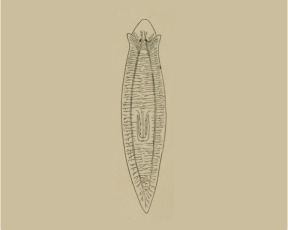
\includegraphics[keepaspectratio]{Francis_Masters_Thesis_files/figure-pdf/fig-Planarian_CNS-1.png}}
\end{center}

{\noindent \emph{Note.} Figure 28 from Jordan, D. S. \& Heath, H. (1902)
Animal Forms; a Second Book of Zoology, public domain}

\end{figure}

The physiologist August Krogh posited that ``You will find in the lower
animals mechanisms and adaptations of exquisite beauty and the most
surprising character'' (\citeproc{ref-krogh_progress_1929}{Krogh, 1929,
p. 203}). The conservation of neurochemistry in planaria is noteworthy.
But it is their regenerative ability that makes them worthy of Krogh's
dictum. Many planaria species undergo a natural form of fission as part
of their reproductive cycle. They tear themselves in half, with each
half then regrowing all the necessary parts of its basic body plan to
form a complete planarian again -- a form of reproductive immortality.
Regeneration is not completely novel in nature. Humans can regrow skin,
and salamanders can regrow amputated limbs. But what sets planaria apart
from the rest of the natural world is their ability to regrow tissue for
the brain and central nervous system.

Planarian regeneration is facilitated by adult pluripotent neoblast
cells which are found throughout the body
(\citeproc{ref-neuhof_vertically-_2016}{Neuhof et al., 2016};
\citeproc{ref-reddien_fundamentals_2004}{Reddien \& Alvarado, 2004}).
After significant injury, these cells proliferate and undergo
differentiation, providing the cell types needed to restore organs,
membranes, and neural networks in the brain. This capability has drawn
interest from medical researchers for more than a century
(\citeproc{ref-child_patterns_1941}{Child, 1941};
\citeproc{ref-morgan_experimental_1898}{Morgan, 1898};
\citeproc{ref-reddien_cellular_2018}{Reddien, 2018}). By understanding
the factors that control planarian regeneration, we may be able to
artificially simulate these processes in humans to restore limbs or
neural structures after injury. Commercial ventures are already being
established in this area. Companies such as Morphoceuticals are looking
to apply lessons learnt from planarian regeneration to rodents and,
pending pre-clinical success, eventually humans
(\citeproc{ref-pio-lopez_morphoceuticals_2023}{Pio-Lopez \& Levin,
2023}; \citeproc{ref-saltzman_boston_2023}{Saltzman, 2023}).

\subsubsection{Review of the Planarian Memory
Literature}\label{sec-review-of-planarian-memory-literature}

In the 1900's, there was still some debate regarding whether
invertebrates have the cognitive means needed to learn. A skeptical
approach was evident from Donald Jensen in the 1970s who posited that
``no invertebrate, no matter how complex is capable of showing `true
learning'\,'' (quoted in \citeproc{ref-rilling_mystery_1996}{Rilling,
1996, p. 591}). This view established an artificial barrier separating
organisms that suitably model human cognition from those that do not.
Because invertebrates were overlooked, researchers tried to make
progress on the neurobiology of memory using the complex nervous systems
of rodents. After many years searching for the rodent engram, the
collection of neurons underlying a specific learning event, this venture
unearthed little of value
(\citeproc{ref-mcconnell_manual_1967}{McConnell, 1967, pp. 2--3}). A
group of psychologists including James McConnell in the 1970s were aware
that little progress was being made in this endeavor. The group moved
defiantly away from rodents and drifted towards invertebrates. Starting
with much simpler organisms would allow researchers to progress past
mere descriptions and arrive at an actual understanding of the
mechanisms of learning.

At first, McConnell and colleagues completed basic experiments showing
that planaria could learn to associate a light (conditioned stimulus,
CS) with a shock (unconditioned stimulus, US)
(\citeproc{ref-mcconnell_effects_1959}{McConnell et al., 1959}).
Compared to control subjects, trained planaria would exhibit more body
contractions in response to light and perform more changes of direction.
But criticism arose over the lack of controls in these experiments
(\citeproc{ref-travis_replicating_1981}{Travis, 1981}). Later follow ups
included blinding the experimenter and testing for confounding factors
such as pseudo-conditioning (where additional stimuli elicit the
unconditioned response despite no temporal relationship) and
sensitisation (an increase in responding to the CS due to repeated
presentation, rather than because of its association with the US).
Contrary to the expectations of psychologists at the time, evidence for
learning in invertebrates accrued study after study. It was eventually
impossible to deny the ability to form stable associative memories to
these rudimentary creatures. McConnell and others such as Eric Kandel
established definitively that invertebrates are capable of learning,
retaining, and acting on information.

Forming associative memories is an impressive feat given the bare-bones
layout of the planarian brain. But why pursue planaria as a model
organism? Why not shift all our resources towards other sophisticated
invertebrates like honeybees and fruit flies? It was the pairing of a
capacity to learn with the rare ability for regeneration in planaria
that sprouted one of the most peculiar branches of research to date: the
investigation of memory retention after decapitation and regeneration of
the brain. This unique combination allowed researchers to ask what
happens if you condition a planarian then cut it in half? Does the tail,
which needs to regenerate its head and central nervous system, retain
any prior learning? James McConnell, alongside Allan Jacobson and Daniel
Kimble were the first scientists to pose and pursue an answer to this
question (\citeproc{ref-mcconnell_effects_1959}{McConnell et al.,
1959}). Across a range of different training procedures, McConnell and
colleagues found that regenerated planarian tails indeed retain
information. This challenged the intuition that memories could only ever
be stored in the brain, at least in some instances
(\citeproc{ref-mcconnell_manual_1967}{McConnell, 1967}). Instead,
through some mechanism, memories are stored or backed up outside the
brain and can be reinstantiated in the new brain during regeneration.

Due to controversial studies on the mechanism of memory persistence,
interest in planaria eventually waned
(\citeproc{ref-rilling_mystery_1996}{Rilling, 1996}). Thirty years
later, this area underwent a modern resurgence thanks to the work of
Shomrat and Levin (\citeproc{ref-shomrat_automated_2013}{2013}). The
authors published an important paper which used an automated training
protocol to revisit the memory retention effect. Planaria, like rodents,
are hesitant to approach food in the center of a novel environment
(\citeproc{ref-best_protopsychology_1963}{Best, 1963b}). They will first
explore the territory, and only then engage in consumption. As planaria
become familiar with the environment through repeated trials, they begin
to approach the food more quickly, demonstrating a form of recognition
memory (\citeproc{ref-best_protopsychology_1963}{Best, 1963b}). The
authors explored whether this type of memory persists in the tails of
trained planaria following complete regeneration of the brain.

Over ten consecutive days, half of the planaria were fed on the novel
rough surface (``familiar'' planaria) while the other half were only fed
on a common smooth surface (``naive'' planaria). At the end of the
training period, the familiar group took a significantly shorter amount
of time to approach and consume the food in the rough environment. Both
groups were then bisected into head and tail halves and left to
regenerate for 10-14 days. The authors then looked at whether the tail
regenerates of familiar planaria retained familiarity of the rough
environment and thus approached food more quickly compared to the naive
tail offspring. The data revealed that regenerated tail fragments from
familiar planaria did approach the food more quickly, however, this did
not reach statistical significance. After undergoing the same training
procedure as the original planaria, the authors found that regenerated
tail fragments from familiar planaria demonstrated a form of memory
savings. The familiar tail regenerates became accustomed to the rough
environment faster than regenerates of control planaria. This indicated
that some memory trace from prior training survived brain regeneration
but required repetition of the training process for the memory savings
to be expressed.

More recently, Samuel et al.
(\citeproc{ref-samuel_addiction-related_2021}{2021}) corroborated this
puzzling memory retention effect. The authors used sucrose to shift the
surface preference of planaria from their innate preference for a smooth
surface to the sucrose-paired rough surface. After amputating the
planaria and allowing time for head regeneration, it was observed that
the tail halves retained the sucrose-paired rough preference, despite
the newly regenerated brain never having been exposed to the rough
surface. In contrast, the tail halves of control planaria -- which were
exposed to the rough surface but did not receive sucrose in this
environment -- showed the expected initial preference for the smooth
surface.

Memory retention experiments presuppose that although a brain is not
necessary for memory storage, it is needed to act upon the memories. For
this reason, sufficient time is always allotted for the brain to
regenerate. However, a recent preprint by Shimojo et al.
(\citeproc{ref-shimojo_preservation_2022}{2022}) challenges this
assumption. They tested whether planarian tails can show retention of a
conditioned response prior to regeneration of the brain. In this study,
planaria were trained to associate a neutral weak UV light (conditioned
stimulus) with an aversive shock (unconditioned stimulus). The shock
typically causes planaria to twist their body -- an unconditioned
contortion response. After pairing the light with the shock, planaria
will display a conditioned contortion response to the UV light alone. On
the second and third day after dissection, well before the brain is
thought to be reformed, the tail halves were exposed to the conditioned
stimulus over a number of trials and their responses were recorded. The
authors analysed the data using a deep neural network to classify
behaviour. They found that most responses from the tail halves were
similar to those produced by an electric shock rather than those
produced by a neutral ultraviolet light. Ultimately, this suggested the
tail halves retained the conditioned behaviour and were able to act on
it despite lacking a brain at the time.

Rhodes and Vierick (\citeproc{ref-rhodes_effects_2024}{2024}) followed a
similar procedure to establish conditioned negative phototaxis in
planaria (moving away from light). Typically, planaria are strongly
averse to blue light, mildly averse to green light, and are indifferent
to red light (\citeproc{ref-paskin_planarian_2014}{Paskin et al.,
2014}). Planaria were trained to associate a neutral red light with an
aversive green light across 5 days. After conditioning, half of the
planaria were bisected into head and tail halves. Three weeks later, all
planaria were tested for retention of the conditioned response. Both
head and tail regenerates retained the conditioned memory as well as
intact planaria. Moreover, memory retention was not statistically
different when comparing head regenerates to tail regenerates. This
study adds to the evidence suggesting that tail regenerates can retain
and act on a memory even after total loss of the brain.

There are a number of issues with the study by Rhodes and Vierick, which
represent common limitations in the planarian literature. First, the
number of planaria per group was very small. Most contained just four to
six subjects. Another key issue is it was not clear how the dependent
variable was operationalised. For example, how much movement was
necessary to qualify as negative phototaxis on a given trial? We must
maintain skepticism for individual studies given their limitations. But
the number of findings showing successful retention of learning through
regeneration provides strong support for the phenomenon.

Classical conditioning procedures are common in the planarian
literature, but some experimenters have also employed operant
conditioning methods
(\citeproc{ref-chicas-mosier_new_2015}{Chicas-Mosier \& Abramson, 2015};
\citeproc{ref-crawford_operant_1967}{Crawford \& Skeen, 1967}; see
\citeproc{ref-best_behavior_1963}{Best, 1963a} for a review of early
studies). A simple learning procedure known as the Van Oye maze was one
of the first forms of reinforcement learning in planaria
(\citeproc{ref-raffa_analysis_2008}{Nicolas et al., 2008};
\citeproc{ref-van_oye_over_1920}{Oye, 1920};
\citeproc{ref-wells_training_1967}{Wells, 1967}). In the typical setup,
planaria are housed in a beaker and a fishing line with food is
suspended just below the water surface. Planaria can detect the presence
of food and navigate towards it (\citeproc{ref-ash_chemical_1973}{Ash et
al., 1973}; \citeproc{ref-miyamoto_chemotaxis_1985}{Miyamoto \&
Shimozawa, 1985}). Planaria must navigate up the wall, across the
surface and down the line to reach the food. This is a low probability
behaviour, but some small percentage will find their way to the fishing
line and be reinforced by the food.

Many planaria will learn to reliably perform this chain of behaviour
when food is present in the environment. Control planaria, on the other
hand, undergo the same procedure but without the food reward attached.
At test, food is not placed on the rod, but is instead dissolved in the
water beforehand. The dissolved food is a cue that food is available.
Trained planaria are subsequently found in much greater numbers on the
suspended line compared to control subjects. Across five experiments
performed by Wells, an average of \textasciitilde17 trained subjects
were found on the line at test compared to an average of
\textasciitilde3 experimental subjects (reviewed in
\citeproc{ref-corning_planarian_1970}{Corning \& Riccio, 1970}). This
procedure demonstrated that planaria can be trained using reinforcement
learning.

Another operant conditioning study was conducted by Corning
(\citeproc{ref-corning_retention_1966}{1966}) during the height of
planaria fame. Corning wondered whether operant conditioned behaviours
could persist through regeneration. Using a T-shaped apparatus, planaria
were trained via positive reinforcement to select their least preferred
side. Reinforcement consisted of being returned to the home arena for 10
minutes after making a correct choice. After incorrect choices planaria
were taken to the start of the maze for another trial. A threshold for
successful learning was set at nine out of ten consecutive correct
choices across trials. Planaria that met this threshold were bisected.

After a two to three week regeneration period, the regenerates (both
heads and tails) were given a baseline preference test and were
subsequently conditioned to criterion. Corning found that the baseline
of trained tail regenerates differed significantly from the baseline of
the original planaria, while untrained planaria tail regenerates did not
differ from the original subjects. This suggested that the trained tail
regenerates retained the prior learned preference, implying that operant
conditioned behaviour can be retained outside of the planarian brain.
Furthermore, the regenerates of trained planaria could also be
conditioned to threshold faster than regenerates of untrained planaria.
While this provided evidence of memory savings when re-exposed, it also
demonstrated a form of uncued recall of the memory.

Building on some of the earliest work on operant conditioning in
planaria, Read (\citeproc{ref-read_reinforcing_2021}{2021}) investigated
whether a Y-shaped maze can be used to shape a directional preference in
planaria. Baseline directional preferences were obtained for planaria by
allowing them to complete six trials in the Y-maze and recording whether
they entered the left or right arm more often. The planaria then
underwent a conditioning procedure. In experiment two, planaria were
rewarded with 2\% ethanol if they entered their non-preferred arm
(``active arm''). On day four of conditioning, planaria entered the
active arm significantly more often than during baseline. This provides
preliminary evidence that planaria may be capable of learning a
directional preference in a Y-maze. Importantly, the behaviour was only
significantly different from baseline on day four (the final day), and
it was therefore not clear whether this conditioned response was stable
or the result of chance variation. Optional stopping may have increased
the chance of a false positive findings within this study, as the number
of conditioning days differed between experiments.

A related study investigated the ability for planaria to be conditioned
in a Y-maze using cocaine as the reinforcing agent (unpublished data,
Canales laboratory). After assessment of the baseline preference, the
non-preferred arm was reinforced with cocaine across three conditioning
days, with three trials each day. Cocaine treated planaria showed a
strong rapid increase in active arm entries, choosing the cocaine
reinforced arm more than 90\% of the time across the final two days of
conditioning. This effect was replicated among another group of
subjects. Other groups were also run which received cocaine in
conjunction with different doses of either ceftriaxone or
N-acetylcystein -- there was no vehicle only group. In general, Planaria
treated with ceftriaxone or N-acetylcystein alongside cocaine did not
acquire a conditioned response.

The experiments above provide preliminary evidence that planaria can
learn an operantly conditioned response. But when considering whether
this behaviour can persist through bisection and regeneration, there is
very limited evidence. Much of the research on operant conditioning in
planaria dates back to the mid-twentieth century. Although historical
research still holds value, modern psychological science has raised
questions regarding the reliability and replicability of past
experiments.

Recent evidence suggests that the psychological literature broadly
considered has oversold the robustness of many psychological phenomena
(\citeproc{ref-open_science_collaboration_estimating_2015}{Open Science
Collaboration, 2015}). Much effort is being devoted towards identifying
the types of decisions which lead to unreliable results appearing in the
literature (\citeproc{ref-simmons_false-positive_2011}{Simmons et al.,
2011}). Interestingly, many scientists openly admit that they have
engaged in questionable research practices -- design and analysis
decisions which lead to untrustworthy results that fail to replicate
(\citeproc{ref-gopalakrishna_prevalence_2022}{Gopalakrishna et al.,
2022}). While replication attempts may often focus on findings from the
last two decades, we must also carry over this skepticism to research
from the twentieth century. Especially in cases where there are only one
or two reports of a given phenomenon. For this reason, we must seek to
establish reliable methods for inducing operant conditioned behaviours
in planaria. Furthermore, we should withhold judgement on whether
learned behaviours can persist through decapitation and regeneration in
planaria until the phenomenon is replicated.

\subsubsection{Positive Reinforcement of Planarian
Behaviour}\label{positive-reinforcement-of-planarian-behaviour}

Investigators have used many different stimuli, both aversive and
appetitive, in their efforts to condition planaria. Cocaine is one of
the most common appetitive stimuli used to date, which acts primarily on
the dopamine transporter. Importantly, these proteins are abundant in
planaria (\citeproc{ref-algeri_effects_1983}{Algeri et al., 1983};
\citeproc{ref-buttarelli_neuropharmacology_2008}{Buttarelli et al.,
2008}). Cocaine is a cost-effective tool for conditioning given the
small quantity needed to reward planaria. But there are some concerns
that require consideration when administering cocaine in behavioural
tasks. For example, cocaine induces strong effects on locomotion and
atypical behaviours at some doses
(\citeproc{ref-pagan_planarians_2013}{Pagán et al., 2013};
\citeproc{ref-rawls_first_2010}{Rawls et al., 2010}).

Cocaine exerts its agonistic effects by blocking reuptake of dopamine
through the dopamine transporters. In humans, this results in more
dopamine activity in the synapse and therefore altered neural activity
in downstream neurons, particularly in the meso-limbic pathway
connecting the ventral tegmental area to the nucleus accumbens
(\citeproc{ref-nestler_molecular_2019}{Nestler \& Lüscher, 2019}). This
agonistic effect is linked to the high that cocaine users experience, an
effect shared by all drugs of abuse
(\citeproc{ref-pierce_mesolimbic_2006}{Pierce \& Kumaresan, 2006}).
Cocaine also acts on serotonergic and noradrenergic transmission by
blocking their respective transporters
(\citeproc{ref-galli_sodium-dependent_1995}{Galli et al., 1995};
\citeproc{ref-mateo_role_2004}{Mateo et al., 2004}). The noradrenergic
effects are thought to stimulate the sympathetic nervous system by
blocking reuptake of noradrenaline and decreasing sympathetic nerve
discharge, resulting in effects such as increased blood pressure and
heart rate (\citeproc{ref-freye_pharmacology_2009}{Freye, 2009};
\citeproc{ref-jacobsen_effects_1997}{Jacobsen et al., 1997};
\citeproc{ref-nestler_molecular_2019}{Nestler \& Lüscher, 2019}).

Amaning-Kwarteng et al.
(\citeproc{ref-amaning-kwarteng_relapse_2017}{2017}) explored the
establishment and extinction of a cocaine-reinforced texture preference.
They found that planaria can be conditioned using cocaine to shift their
surface texture preference from smooth to rough and that this preference
can be extinguished (reverted back to the original preference) after
repeated exposure without reinforcement. Subsequently, exposure to a
bath of cocaine was enough to reinstate the conditioned preference when
given free access to both surfaces.

Building on prior work dating back to the 1960's
(\citeproc{ref-needleman_tolerance_1967}{Needleman, 1967}), Mohammed
Jawad et al. (\citeproc{ref-mohammed_jawad_dissociation_2018}{2018})
investigated addiction like behaviour in planaria through conditioning,
extinction and tolerance. The experiment successfully demonstrated a
conditioned place preference (CPP), extinction of the preference, and
context specific tolerance. Of particular significance, this work
demonstrated that sucrose induced CPP requires dopaminergic activity.
Administration of a dopamine D1 antagonist during conditioning blocked
acquisition of CPP but did not interfere with context specific
tolerance. An interesting dissociation that may have implications for
understanding addiction in humans.

Understanding the molecular and circuit dynamics underpinning addiction
may allow us to interface with the brain so as to reduce maladaptive
behaviours. Currently, therapies focus on top-down strategies. People
are coached to recognise their thoughts and emotions related to drugs
and to manage them rather than act on them. However, if the chemistry
and structural wiring of the brain change during the acquisition of an
addiction, top-down strategies may be inadequate. bottom-up therapies
involving a change of the bodies chemical and molecular milieu may
support the unraveling of these harmful brain adaptations
(\citeproc{ref-chodkiewicz_conceptual_2023}{Chodkiewicz, 2023}). We are
not in a position to experiment freely with bottom-up interventions in
humans or other mammals. In place of that, planaria enable us to pursue
a deeper understanding of the chemical and molecular changes underlying
habit formation and the identification of targeted interventions to
reduce future drug seeking behaviour.

\subsection{Unresolved Questions}\label{unresolved-questions}

In the first half of the 20th century, there was doubt regarding whether
invertebrates can learn. But as we look back nearly a century later, we
have gathered ample evidence that planaria and many other invertebrates
can form long-lasting memories
(\citeproc{ref-amaning-kwarteng_relapse_2017}{Amaning-Kwarteng et al.,
2017}; \citeproc{ref-samuel_addiction-related_2021}{Samuel et al.,
2021}; \citeproc{ref-wells_training_1967}{Wells, 1967}). Planaria are an
especially useful organism given their ability to learn and their unique
ability to regenerate. As has been shown with conditioning procedures,
there is now evidence that memory can be successfully retained outside
of the brain (\citeproc{ref-shomrat_automated_2013}{Shomrat \& Levin,
2013}). The persistence of basic associative memory through regeneration
is remarkable. But a more compelling finding that would truly shake our
fundamental understanding of memory storage mechanisms would be the
persistence of complex behavioural responses.

An acquired texture preference is a valid form of learning. But it is
far removed from the memories that concern us in our day to day lives.
In contrast, learning shaped by a reward better reflects the intentional
learning we associate with intelligence and meaningful behaviour in
humans. If complex memories formed by operant conditioning can persist
in planaria despite complete loss of the brain, this may have profound
implications for the way we view memory storage and retrieval in humans.
This project aims to extend the phenomenon of memory retention through
regeneration shown for classical conditioning to an operant conditioned
behaviour.

Shomrat and Levin (\citeproc{ref-shomrat_automated_2013}{2013}) observed
that familiar tail regenerates did not initially show evidence of memory
retention. However, it was clear that their performance on the task
improved more rapidly than controls when they were exposed to the
training procedure. Some fragment of memory for the context must have
survived outside the brain. The authors showed this memory benefited
future performance after re-exposure to the training procedure. What
remains unknown is whether retraining is the only process that supports
reinstantiation of the previously acquired memory. Could it be that
other contextual cues, such as exposure to the reinforcing stimulus
alone, are sufficient to bring back memories acquired before
decapitation?

The results of Shomrat and Levin
(\citeproc{ref-shomrat_automated_2013}{2013}) suggested the memory trace
lay dormant and failed to be reactivated at first. After exposure to the
same training procedure that led to the original memory formation, the
dormant trace was then reawakened. This phenomenon of memory
reactivation after prior failures parallels behaviour reinstatement in
addiction research. After successfully training an animal to lever press
for a reward such as cocaine, the lever press response can be
extinguished by allowing the animal to repeatedly engage in the
behaviour without being rewarded
(\citeproc{ref-de_wit_reinstatement_1981}{Wit \& Stewart, 1981}).
Eventually the animal will stop performing the conditioned response when
the lever is presented. However, if the animal is exposed to the
reinforcing stimulus before being placed back in the operant chamber,
the lever pressing behaviour will spontaneously return
(\citeproc{ref-de_wit_reinstatement_1981}{Wit \& Stewart, 1981}).

With respect to both phenomena, the memory is either not accessible or
is not acted upon and requires exposure to the right stimulus to be
reactivated. Although extinction and reinstatement of drug seeking
behaviour has been modeled in planaria
(\citeproc{ref-amaning-kwarteng_relapse_2017}{Amaning-Kwarteng et al.,
2017}), no experiments have explored whether a reinstatement procedure
can also be used to reactivate memories which are dormant after
decapitation and regeneration. The phenomena of memory saving among
regenerates demonstrate that some memory trace is retained in the
brainless tail half. Perhaps this trace can be reactivated without the
need for retraining by instead exposing the tail regenerates to the
reinforcing stimulus. This project will therefore investigate whether
memory stored outside the brain behaves like an extinguished memory such
that exposure to the reinforcing stimulus is sufficient to reinstate the
memory trace.

\section{Experiment 1}\label{sec-experiment-1}

Experiment 1 aimed to find a dose of cocaine that would not
significantly alter the locomotive behaviour of planaria. To increase
the likelihood that our selected dose was still rewarding despite a lack
of effect on movement, we used a range of doses that have been reported
to show effective conditioning in the literature. Cocaine has been
regularly used in planaria research to establish models of addictive
behaviour and to understand its toxicity and synergistic effects when
combined with other drugs
(\citeproc{ref-amaning-kwarteng_relapse_2017}{Amaning-Kwarteng et al.,
2017}; \citeproc{ref-hutchinson_persistent_2015}{Hutchinson et al.,
2015}; \citeproc{ref-palladini_pharmacological_1996}{Palladini et al.,
1996}; \citeproc{ref-raffa_description_2005}{Raffa \& Desai, 2005};
\citeproc{ref-tallarida_ethanol_2014}{Tallarida et al., 2014}). Studies
focused on classical conditioning, often for the purpose of modelling
addictive behaviour, have used doses ranging from 1μM
(\citeproc{ref-hutchinson_persistent_2015}{Hutchinson et al., 2015}) to
80μM (\citeproc{ref-raffa_cocaine_2005}{Raffa et al., 2005}).

Investigators have observed that some planaria species are more amenable
to conditioning procedures than others
(\citeproc{ref-mueller_use_2002}{Mueller \& Levin, 2002};
\citeproc{ref-samuel_addiction-related_2021}{Samuel et al., 2021}).
Differences in the behaviour and responses of planarian species have
been observed in response to several types of stimuli
(\citeproc{ref-cochet-escartin_scrunching_2015}{Cochet-Escartin et al.,
2015}; \citeproc{ref-debold_differences_1965}{DeBold et al., 1965}). The
species used throughout this project likely differs from those used
elsewhere in the literature and may in fact be a species indigenous to
New Zealand, although its identity is, as yet, unknown. For this reason,
it is important to identify a suitable dose of cocaine which does not
significantly alter motility.

\subsubsection{Colony Maintenance and
Handling}\label{colony-maintenance-and-handling}

Due to restrictions on importing identified species such as
\emph{Schmidtea mediterranea} into New Zealand, local planaria were
sourced from a local stream within Wellington, New Zealand. Given the
basic characteristics of the planaria (colour, head shape etc.) it is
thought that there is a combination of \emph{Cura} and \emph{Neppia} --
both of which are commonly found in New Zealand waterways. We intend to
perform genomic analysis at a later date to confirm the species
identity. Prior to collection for this experiment, planaria were housed
in a 50 liter glass aquarium with internal filtering. The aquarium
contained a natural ecological environment (rocks, snails, algae etc.).
The tank water (referred to as ``planaria water'' hereafter) was
maintained with Prime -- a concentrated water conditioner. Planaria were
fed between one and three times a week, with meals consisting of frozen
liver paste. The colony was maintained on a 12-hour light/dark cycle
with lights on at 9:30am till 9:30pm. For this experiment, planaria were
handled using either a filbert (medium length flat) paintbrush or a fine
artist's paintbrush.

\subsubsection{Materials and Procedure}\label{materials-and-procedure}

Plastic petri dishes with a diameter of 5.5cm were used to assess
motility. Petri dishes contained a final solution of 8ml, made up of
planaria water for control subjects and cocaine hydrochloride mixed with
planaria water for experimental subjects. Planaria locomotion was
captured using an OPPO A17 smart phone and the videos were imported into
EthoVision (Noldus Information Technologies, Wageningen, the
Netherlands) for motility tracking. When subjects were not visible due
to being occluded by a shadow or dish wall (\textasciitilde10\% of
frames on average across all subjects), missing data were interpolated
using the interpolation feature in EthoVision. This imposed a direct
line from the subject's last location to the next observed location to
determine the distance traveled.

60 planaria were used in this experiment. Planaria were assigned to one
of six dose conditions based on those commonly used in the planarian
literature. This included 0, 1, 5, 10, 20 and 100μM (\emph{n} = 10 per
condition). Subjects were run across twelve recording
sessions\sidenote{\footnotesize The first ten sessions each contained one subject from
  the 0 - 20μM conditions, whereas the last two session only contained
  subjects in the 100μM condition. This is because the 100μM condition
  was added after the initial data were analysed to ensure that the
  cocaine was having some effect on the planaria and was not inert.}.
Subjects were collected from the breeding tank on the day of data
collection. Within each session, subjects were randomly allocated to
their condition using a freely available
\href{https://stattrek.com/statistics/random-number-generator\#table}{random
number generator}.

Each dose-response session lasted 15 minutes. Prior to the first
recording session of the day the drug concentrations were achieved by
mixing cocaine (dissolved in distilled water) with planarian water to
reach a final solution of 8ml. Each solution was mixed and allowed to
sit for several minutes to ensure diffusion of the drug. For each
session, planaria were picked up at random and a randomly generated
number sequence was used to determine which condition it was assigned
to. The recording began once all five subjects were in their respective
dishes. After completing a single trial, planaria were rehoused in a
large tank and were not used for any subsequent experiments in this
manuscript.

Figure~\ref{fig-Dose_response_apparatus} shows the recording setup used
for this experiment. Five petri dishes were positioned on a white
acrylic sheet. Recording sessions took place under red light, with the
light positioned 36cm above the dishes. The dishes were aligned in a 2x3
grid, with a gap left in the top middle position. The overhead light was
centered here to minimise shadows cast over the dishes -- this was
important for digital tracking accuracy. Each drug concentration was
rotated across the 5 grid positions between trials to control for any
effects of lighting angle.

\begin{figure}[!htbp]

{\caption{{Graphical Depiction of the Dose response
apparatus}{\label{fig-Dose\_response\_apparatus}}}}

\begin{center}
\pandocbounded{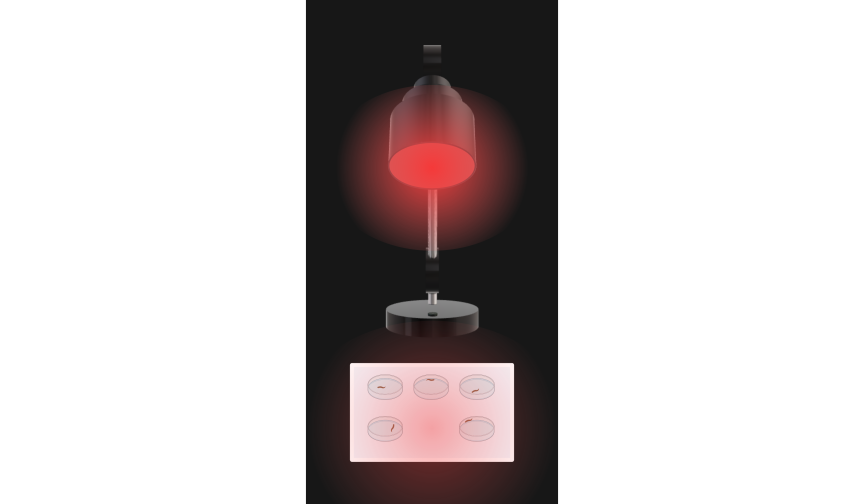
\includegraphics[keepaspectratio]{Francis_Masters_Thesis_files/figure-pdf/fig-Dose_response_apparatus-1.png}}
\end{center}

{\noindent \emph{Note.} Graphical depiction of the dose response setup
used to assess planarian motility in response to cocaine. The room was
illuminated by a lamp fitted with red plastic to filter out non-red
light. All other lights were turned off during data collection. The
arrangement of petri dishes and planaria on the white plastic sheet can
be seen below the lamp. A Oppo A17 phone was used to record planaria
motility (not shown in the graphic). The phone was balanced on a clamp
attached to a support stand positioned to the side of the plastic
sheet.}

\end{figure}

\subsubsection{Results and Discussion}\label{results-and-discussion}

Figure~\ref{fig-boxplot} depicts the distance moved by planaria across
the six conditions. Prior to performing any statistics, the assumptions
of normality and homogeneity of variances were tested. Levene's test for
homogeneity of variances suggests there were equal variances across
conditions (F = 1.95, \emph{p} = .101). The Shapiro-Wilk test indicated
that the data were not normally distributed (W = 0.935, \emph{p} =
.003). Due to violation of the assumptions of ANOVA, a Kruskal-Wallis
test was used to evaluate group differences. The results show a
statistically significant effect of condition on distance moved (χ2 (5)
= 11.3, \emph{p} = .045). An exploratory post-hoc Dunn's test was
carried out to determine the group differences. The results indicated
that the 100μM group differed significantly from several other groups:
control (\emph{p} = .006), 5μM (\emph{p} = .002), 10μM (\emph{p} =
.003), and 20μM (\emph{p} = .016). No other significant differences were
found.

\begin{figure}[!htbp]

{\caption{{Plot of planarian motility by
condition}{\label{fig-boxplot}}}}

\begin{center}
\pandocbounded{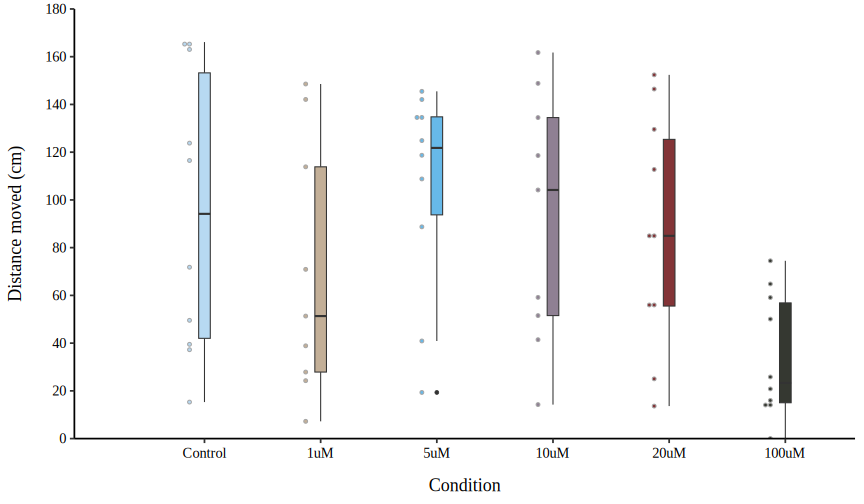
\includegraphics[keepaspectratio]{Francis_Masters_Thesis_files/figure-pdf/fig-boxplot-1.png}}
\end{center}

{\noindent \emph{Note.} Box and whisker plot of distanced moved by
planaria over the 15-minute recording interval. Black bars indicate the
mean distance moved for each condition.}

\end{figure}

The results in Figure~\ref{fig-boxplot} convey the variability of
planarian behaviour. All conditions had at least one subject which moved
less than 30cm over the 15-minute recording, and all groups had at least
two subjects that moved more than 140cm. Experimenter observations
indicate that when placed in the recording dish, some planaria would
move initially, and then come to rest within a few minutes at a spot on
the wall. They would remain here without meaningful movement for the
remainder of the recording. Although the 1μM group did not differ
significantly from the control group, there is a curious grouping of
planaria in the 1μM condition below 60cm. Consistent with this,
Hutchinson et al. (\citeproc{ref-hutchinson_persistent_2015}{2015})
observed a significant decrease in motility during exposure to 1μM of
cocaine but not to 10μM when compared to a control group. No potential
explanation was offered for this unusual curvilinear pattern.

The results suggest any dose between 1μM and 20μM could be used for
conditioning without systematically affecting planaria motility. It was
also necessary to select a dose that was sufficiently rewarding for
planaria. A range of doses have been used to successfully condition
planaria in CPP paradigms. These procedures typically involve low doses
such as 1μM (\citeproc{ref-hutchinson_persistent_2015}{Hutchinson et
al., 2015}), 5μM
(\citeproc{ref-amaning-kwarteng_relapse_2017}{Amaning-Kwarteng et al.,
2017}) or 10μM (\citeproc{ref-hutchinson_persistent_2015}{Hutchinson et
al., 2015}). It is worth noting that in the case of CPP, drug exposure
time is relatively long. On the order of 15-20 minutes per trial.
Whereas in the operant conditioning paradigm proposed in Experiment 2 of
this project, exposure time would be just 3 minutes. To adjust for the
smaller absorption window compared to CPP experiments, the larger 20μM
concentration was chosen for experiment 2.

Alongside total motility, we were able to inspect how planaria motility
changed over the recording interval. We observed that planaria moved
more at the start of the session compared to the end, with a gradual
decrease in the distance moved with each passing minute (see
Figure~\ref{fig-ridgeplot}). An exploratory Welch's two sample t-test
found a significant difference between the time traveled in the first
minute (M = 7.58, SD = 3.29) compared to the 15th minute (M = 4.59, SD =
3.95), with subjects travelling significantly further during minute 15
(t(59) = 6.2, \emph{p} \textless{} .001). In future dose-response
assessments, shorter recording sessions may suffice to assess
dose-response curves.

\begin{figure}[!htbp]

{\caption{{Plot of planarian motility across recording
interval}{\label{fig-ridgeplot}}}}

\begin{center}
\pandocbounded{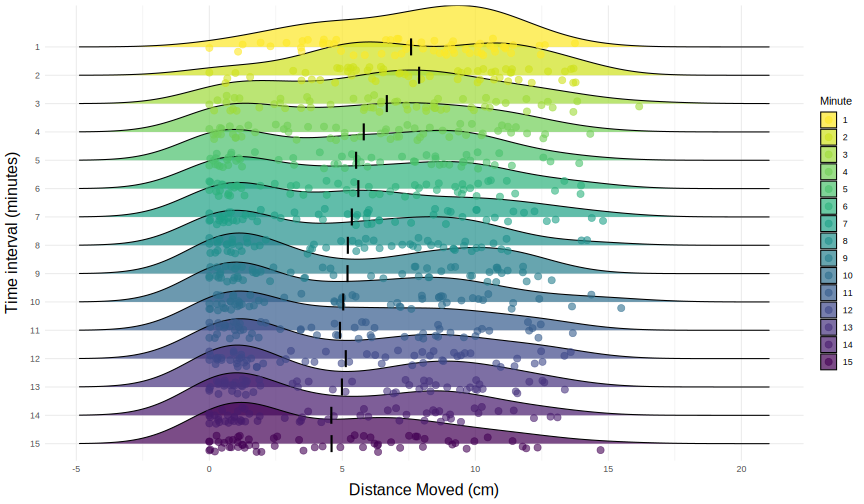
\includegraphics[keepaspectratio]{Francis_Masters_Thesis_files/figure-pdf/fig-ridgeplot-1.png}}
\end{center}

{\noindent \emph{Note.} Ridge plot of distance moved by planaria during
each minute interval. Each ridge shows the distance distribution for all
subjects during the minute interval. Black bars indicate the mean
distance moved for the whole sample (treatment and control subjects).}

\end{figure}

\section{Experiment 2}\label{sec-experiment-2}

Prior research has demonstrated the capacity for learning in planaria by
way of classical conditioning. Moreover, it has been further shown that
classically conditioned memories can be retained after decapitation and
regeneration of the brain
(\citeproc{ref-samuel_addiction-related_2021}{Samuel et al., 2021};
\citeproc{ref-shomrat_automated_2013}{Shomrat \& Levin, 2013}). But the
capacity for complex memories shaped by operant conditioning to persist
under these conditions has not been definitively shown. As a first step
towards assessing whether operantly conditioned memories can persist
through decapitation, we must first demonstrate the capacity for operant
learning in this species of planaria. The power analysis, experimental
design and analysis plan of this experiment were preregistered prior to
data collection. The preregistration can be found online at
\href{https://osf.io/tq7u4/?view_only=9c794dd942fb4a54b6a986c0a893fe46}{Open
Science Framework} and at
\href{https://www.psycharchives.org/en/item/d6109ed1-9aab-467b-b981-e009be95f308}{PsycArchives}.

\subsubsection{Colony Maintenance and
Handling}\label{colony-maintenance-and-handling-1}

The colony maintenance protocols were identical to those described in
Experiment 1. To track subjects throughout the experiment, planaria were
housed individually in 12-well plates with 2ml of planarian water
(changed daily\sidenote{\footnotesize In the waiting period between conditioning and
  the memory retention test, 12 subjects (\#49 - \#60 inclusive) from
  Experiment 1 were left overnight without water due to experimenter
  error. This lead to three immediate deaths. Although the remaining
  subects survived, during the memory retention and reinstatement tests,
  six failed to respond at all and the remaining three subjects only
  responded once or twice.}). Planaria were stored in a room illuminated
with standard white fluorescent lighting on a 12-hour light/dark cycle
with lights on at 9:30am till 9:30pm. Subjects were moved into a room
dimly illuminated with red light while completing their Y-maze trials.
Planaria were handled using different techniques for different
circumstances. When removing planaria from their 12-well-plate, a
filbert (medium length flat) paintbrush was preferred. However, when
moving planaria between petri dishes and the y-maze, a fine artist's
paintbrush was preferred. In other cases, such as when planaria would
sit in the middle of the y-maze divot, a plastic transfer pipette with
the tip cut off was used. Planaria were gently handled throughout their
lifespan. Rough handling was suspected to have caused a high mortality
rate during pilot experiments.

\subsubsection{Materials and
Procedure}\label{sec-2-materials-and-methods}

This experiment used two groups: a treatment group (\emph{n} = 30) which
received cocaine and and a control group (\emph{n} = 30) which received
vehicle only. There were four experimental stages: baseline,
conditioning, test, and reinstatement (see
Figure~\ref{fig-exp2_timeline}). A modified version of the Y-maze
conditioning procedure outlined by Read
(\citeproc{ref-read_reinforcing_2021}{2021}) was adopted. During
baseline and conditioning trials two planaria were run concurrently in
separate Y-mazes (see Figure~\ref{fig-Ymaze_V1_dimensions}). Each maze
was filled with 1.8ml of planaria water which shaken gently to evenly
distribute the water throughout the runway and arms. Six planaria were
used per run, wherein they completed either six (baseline) or four
trials per day (conditioning) with an intertrial interval of
approximately 15 minutes. At the start of each run six planaria were
moved into petri dishes. At the start of a trial, planaria were
transferred to the middle of a maze runway using a paintbrush. Each maze
contained one planarian. A timer was started once each planarian was
placed in the runway. Planaria were given three minutes to enter one of
the arms\sidenote{\footnotesize If the planarian had some part of their body in an arm
  at the end of the allotted time, they would be given up to an extra
  minute to make their decision.}. Once a subject entered an arm, the
plug was inserted to stop liquid moving between compartments, after
which 0.5ml remained in each arm\sidenote{\footnotesize Measured by extracting and
  weighing the volume of distilled water trapped in each arm, assuming a
  density of 1g/ml. Small deviations are inevitable, but this was the
  most common value seen during our tests}. A planarian was considered
to have entered the arm when the plug could be safely inserted without
touching the planarian.

When treatment subjects entered the active arm, 43.5μL of cocaine in
distilled water was pipetted near the center of the arm to achieve a
20μM concentration. If the inactive arm was selected, an identical
volume of distilled water was pipetted near the center of the arm. After
administration, the timer was restarted and three minutes were given for
absorption. For control subjects, entry into either arm resulted in
43.5μL of distilled water (vehicle) into the arm. If a subject failed to
enter an arm, the plug was inserted and 43.5μL of distilled water was
pipetted into the runway and then three minutes were given. The runway
light was on throughout the duration of the trial. At the end of a
trial, planaria were gently removed and placed back into their holding
dish. Mazes were rinsed and dried between each trial.

The memory retention test took place 14 days after conditioning (see
Figure~\ref{fig-exp2_timeline}). At test, six planaria were used per
run. Three planaria were run concurrently in three separate Y-mazes.
Planaria were given three minutes to enter an arm. Once a decision was
made, the plug was inserted and planaria were left for approximately 60
seconds before being moved back to the holding dish. No additional
liquid was added during test trials. The next group of three planaria
would then begin their first test trial. The inter trial interval was
approximately six minutes and thirty seconds. A reinstatement procedure
was carried out the following day. The procedure was identical to the
test stage with the only additional step being drug exposure before the
first trial. At the start of a run, planaria were placed individually
into an 8ml solution planaria water containing 20μM of cocaine for 10
minutes. At the end of the exposure interval, planaria were moved into
separate Y-mazes to begin their first trial. Planaria were only exposed
to cocaine prior to the first reinstatement trial.

There were three exclusion criteria identified in the preregistration
\href{https://osf.io/skfnv?view_only=9c794dd942fb4a54b6a986c0a893fe46}{document}.
The exclusion criteria were: A) failing to complete at least four of the
six baseline trials; B) failing to complete at least two trials on
consecutive conditioning days; C) failing to complete at least four of
the last six trials of conditioning. We attempted to replace all
subjects excluded due to criterion A. However, due to time constraints,
of the 18 that failed to meet this criterion, only 13 could be
successfully replaced. Five subjects could not be replaced and so
started conditioning despite having completed only two or three baseline
trials. Thirteen subjects met criterion B or C and were excluded from
the data analysis. There was no exclusion criteria set for the test and
reinstatement procedure. However, some subjects died in the waiting
period, or demonstrated greatly impaired behaviour at test or
reinstatement and were thus excluded.

Three laser etched Y-mazes were used for this experiment (see
Figure~\ref{fig-Ymaze_V1_dimensions} for dimensions). Mazes were laser
etched into 80x80mm plastic squares. At the intersection between the
runway and the arms, there was a small divot on the floor of the maze.
This allows a plug to be inserted to trap liquid in the arms and enable
controlled drug administration. The maze floor contained subtle lines as
a result of the etching process. At the base of the runway there was a
small externally powered white light (\textasciitilde20 lux) which was
fixed into the plastic. Light is an aversive stimulus which induces
negative phototaxis and should discourage planaria from resting at the
start of the runway.

\begin{figure}

\caption{\label{fig-exp2_timeline}Graphical Timeline of Experiment 2}

\centering{

\pandocbounded{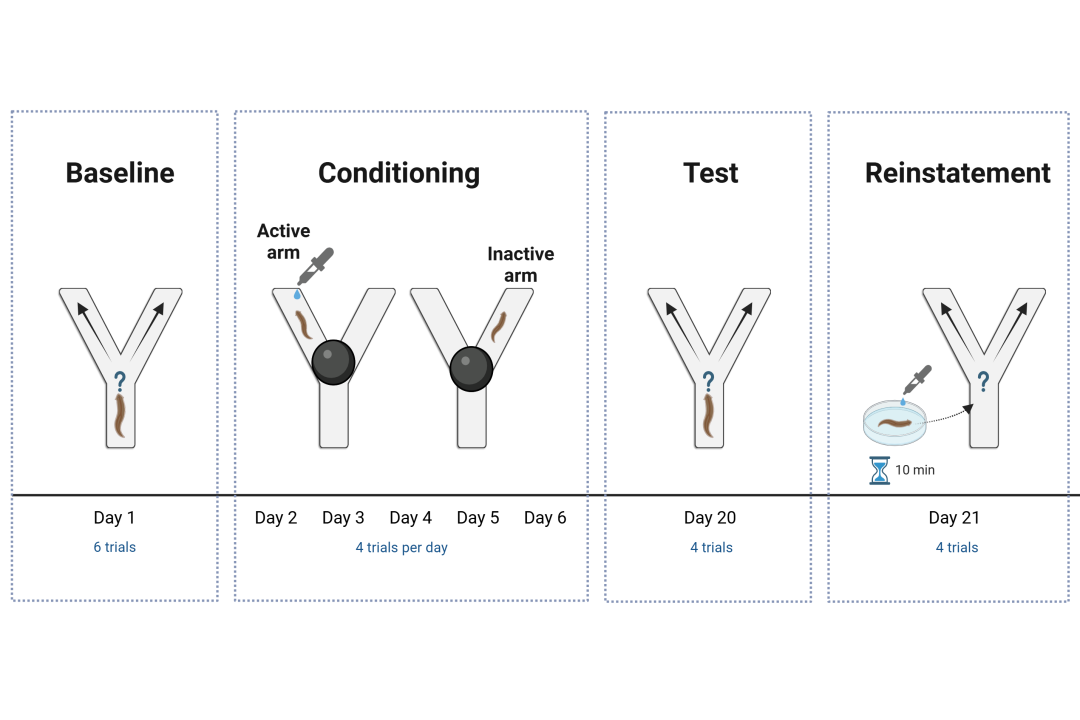
\includegraphics[keepaspectratio]{Francis_Masters_Thesis_files/figure-pdf/fig-exp2_timeline-1.png}}

}

\end{figure}%

\begin{figure}[!htbp]

{\caption{{Laser etched plastic
Y-maze}{\label{fig-Ymaze\_V1\_dimensions}}}}

\begin{center}
\pandocbounded{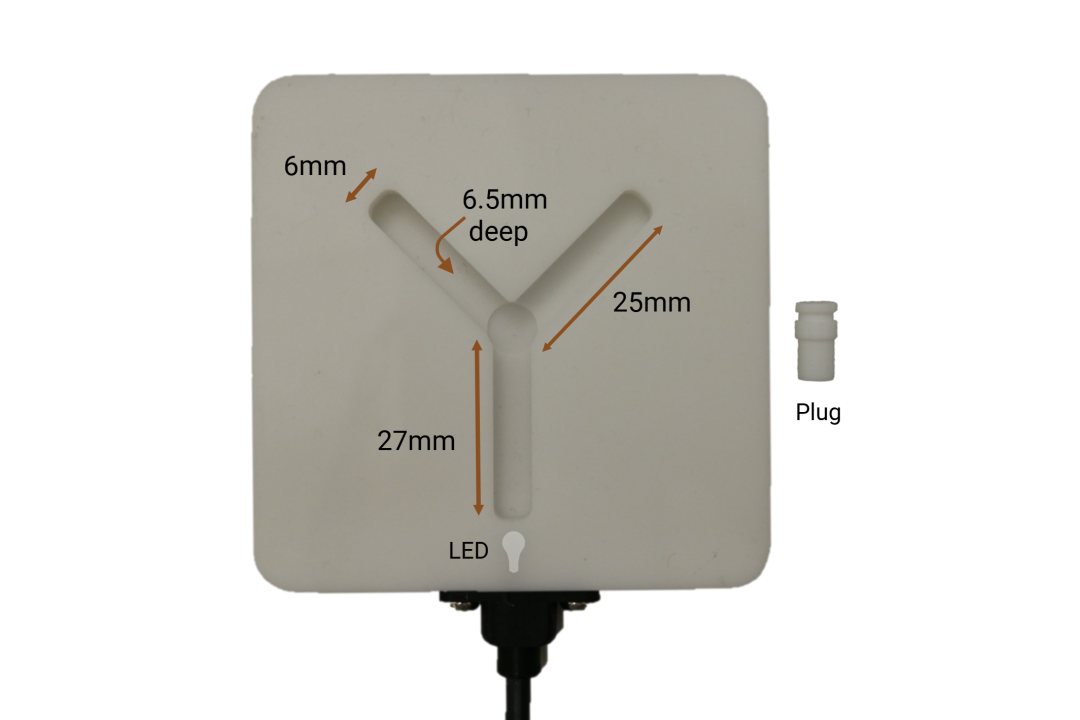
\includegraphics[keepaspectratio]{Francis_Masters_Thesis_files/figure-pdf/fig-Ymaze_V1_dimensions-1.png}}
\end{center}

{\noindent \emph{Note.} The Y-maze depicted here was laser etched into
white 80x80mm plastic plates. A white LED was drilled into the maze at
the start of the runway to induce negative phototaxis (light bulb symbol
is indicative of LED location beneath the plastic). The light was
powered by a 9V power adapter. A plastic plug was also etched out of
plastic to stop liquid moving between compartments after a planarian
entered one of the arms.}

\end{figure}

\subsubsection{Results and Discussion}\label{results-and-discussion-1}

Of the 60 original subjects, three died during conditioning (two control
subjects and one treatment subject) and another six subjects died
throughout the regeneration period (five control subjects and one
treatment subject). The initial deaths were attributed to repeated
handling with a paintbrush, while the deaths during regeneration were in
part due to 12 subjects being left overnight with no water.
Additionally, 10 other subjects were excluded due to meeting one or more
of the exclusion criteria during conditioning. Of the subjects excluded
due to death or meeting the exclusion criteria, 9 were control subjects
and 4 were treatment subjects. Due to different requirements for the
between groups and within subjects comparisons for active arm entries,
and due to some subjects having no data for the decision latency
analysis, there were different numbers of subjects for the comparisons
at each time point. For this reason, the number of subjects per
condition at each time point have been included in the figures shown
below.

After removing subjects that met the exclusion criteria, the majority of
subjects had an initial preference towards the right arm (\emph{n} =
25), with just over a quarter favouring the left arm (\emph{n} = 13) and
several having no preference (\emph{n} = 9). This experiment employed a
biased design, such that the active arm to be reinforced was the
opposite of the initial preference or randomly assigned for those with
no initial preference. The left arm was active for 28 subjects, and the
right arm was active for 19 subjects. Looking at the baseline
preferences of excluded subjects, there was no systematic bias towards
either arm, with slightly more preferring the right arm (\emph{n} = 6)
than the left arm (\emph{n} = 4), and a few showing no preference
(\emph{n} = 3).

Figure~\ref{fig-exp2decisions} shows the average proportion of trials
for which subjects entered the active arm at each time point. A
generalised linear mixed effects model with family set to binomial was
fitted in R using the lme4 package
(\citeproc{ref-bates_fitting_2015}{Bates et al., 2015}). Subject ID was
set as a random effect, with condition, time point and the interaction
term as fixed effects. Pairwise comparisons with a Bonferroni correction
were carried out using the emmeans package in R
(\citeproc{ref-lenth_emmeans_2024}{Lenth, 2024}). A Type III ANOVA was
conducted using the car package (\citeproc{ref-fox_r_2019}{Fox \&
Weisberg, 2019}) to identify whether there was a significant effect of
condition or time, or an interaction effect.

We did not detect a significant effect of condition (χ2 (1) = 0.773,
\emph{p} = .379). The results indicated a significant effect of time (χ2
(3) = 35.5, \emph{p} \textless{} .001) and a significant time*condition
interaction (χ2 (3) = 10.2, \emph{p} = .017).

Post-hoc pairwise comparisons were carried out using estimated marginal
means with a Bonferroni corrections applied to account for multiple
comparisons. Comparisons looked at within group differences in response
probability across the four phases and between group differences at each
time phase. The effect sizes were reported using Cohen's h which is
appropriate when comparting two proportions
(\citeproc{ref-cohen_statistical_1988}{Cohen, 1988}). There were two
within-group differences for the control subjects: endpoint differed
significantly from baseline (\emph{h} = 0.56, \emph{p} \textless{}
.001), and test differed significantly from endpoint (\emph{h} = 0.65,
\emph{p} \textless{} .001). These differences represent medium effect
sizes (\citeproc{ref-cohen_statistical_1988}{Cohen, 1988, pp.
184--185}). There were three within-group differences for the treatment
subjects: endpoint differed significantly from baseline (\emph{h} = 0.4,
\emph{p} = .002), test differed significantly from baseline (\emph{h} =
0.35, \emph{p} = .044), and reinstatement differed significantly from
endpoint (\emph{h} = 0.36, \emph{p} = .035). These differences represent
small effect sizes, with the baseline-to-endpoint difference approaching
the medium effect size criterion of \emph{h} = 0.5
(\citeproc{ref-cohen_statistical_1988}{Cohen, 1988, pp. 184--185}). A
significant between-group difference was found in the preference score
between treatment and control subjects at test (\emph{h} = 0.48,
\emph{p} = 0.004) which represent a small to medium effect size.
Treatment subjects entered the active arm more often (\emph{M} = 0.427,
\emph{SD} = 0.29) than control subjects (\emph{M} = 0.208, \emph{SD} =
0.177). No other significant between group differences were detected.

\newpage

\begin{figure}[!htbp]

{\caption{{Learning and Memory Retention across two weeks in Cocaine
Treated Planaria}{\label{fig-exp2decisions}}}}

\begin{center}
\pandocbounded{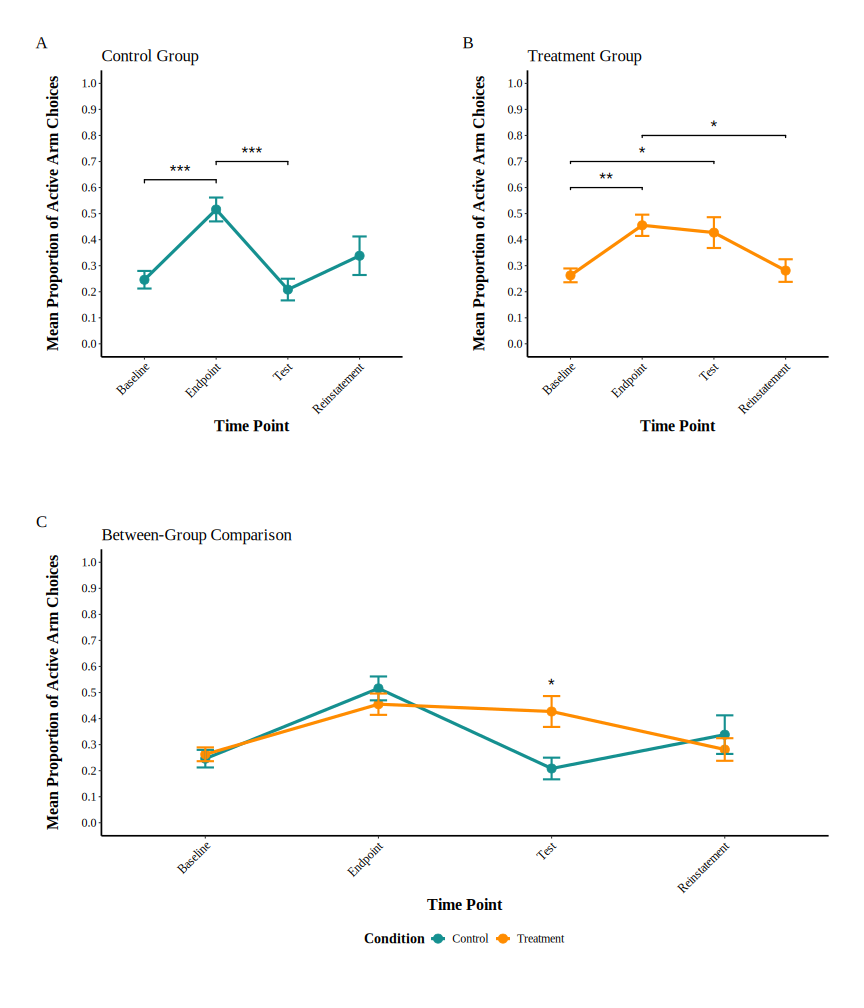
\includegraphics[keepaspectratio]{Francis_Masters_Thesis_files/figure-pdf/fig-exp2decisions-1.png}}
\end{center}

{\noindent \emph{Note.} Changes in Y-maze active arm preference across
experimental phases. The baseline phase included 6 trials, conditioning
endpoint included the final 6 trials of conditioning, and both test and
reinstatement phases included 4 trials each. A) The control group showed
significant differences in active arm entries between baseline and
endpoint, and between endpoint and test. B) Treatment group demonstrated
significant differences between baseline and endpoint, baseline and
test, and endpoint and reinstatement. C) Between-group comparisons
revealed there was a significant difference in active arm entries at the
test phase. Error bars represent standard error of the mean. * = p
\textless.05; ** = p \textless.01; *** = p \textless.001.}

\end{figure}

Looking at the results in Figure~\ref{fig-exp2decisions}B, subjects in
the treatment group showed some evidence of a conditioned response.
These subjects were more likely to choose the active arm at the end of
conditioning (endpoint) compared to baseline. Moreover, this preference
was maintained for two weeks as demonstrated by the heightened active
arm entries at test. Despite the behavioural change persisting for two
weeks, when tested the next day during the reinstatement procedure the
proportion of active arm entries had returned to baseline levels.

Figure~\ref{fig-exp2decisions}shows that the control group demonstrated
a similar increase in active arm entries despite receiving no
reinforcement. However, in contrast to the treatment group, this
returned to baseline levels when tested two weeks after conditioning.
This highlights the natural variability in planaria behaviour over time.

The between groups comparison seen in Figure~\ref{fig-exp2decisions}C
shows a significant difference between groups at test. It may be that
the preference stability shown by the treatment group is evidence of
true learning as opposed to the natural variability of behaviour seen in
the control group. This could explain why the change in behaviour for
the treatment group persisted for two weeks, while the behaviour of the
control group diminished back to baseline levels. Admittedly, the
reinstatement results reduce the credibility of this explanation. If the
conditioned behaviour was able to persist for several weeks, there is
little reason to expect it would be extinguished rapidly but fail to
show the expected effect of reinstatement. Overall, the results provide
preliminary support for the notion that planaria can be conditioned in a
Y-maze and that this response can last at least two weeks.

This experiment also considered planaria response times for each trial.
We hypothesised that even if planaria cannot learn to make the correct
decision, they may demonstrate increased motivation due to being aware
that a reward is available. This could be inferred from faster
responding in the treatment group compared to the control group. The
response time data across the four experimental phases are shown in
Figure~\ref{fig-decision-time}.

\begin{figure}[!htbp]

{\caption{{Decision Latency Across Experimental
Phases}{\label{fig-decision-time}}}}

\begin{center}
\pandocbounded{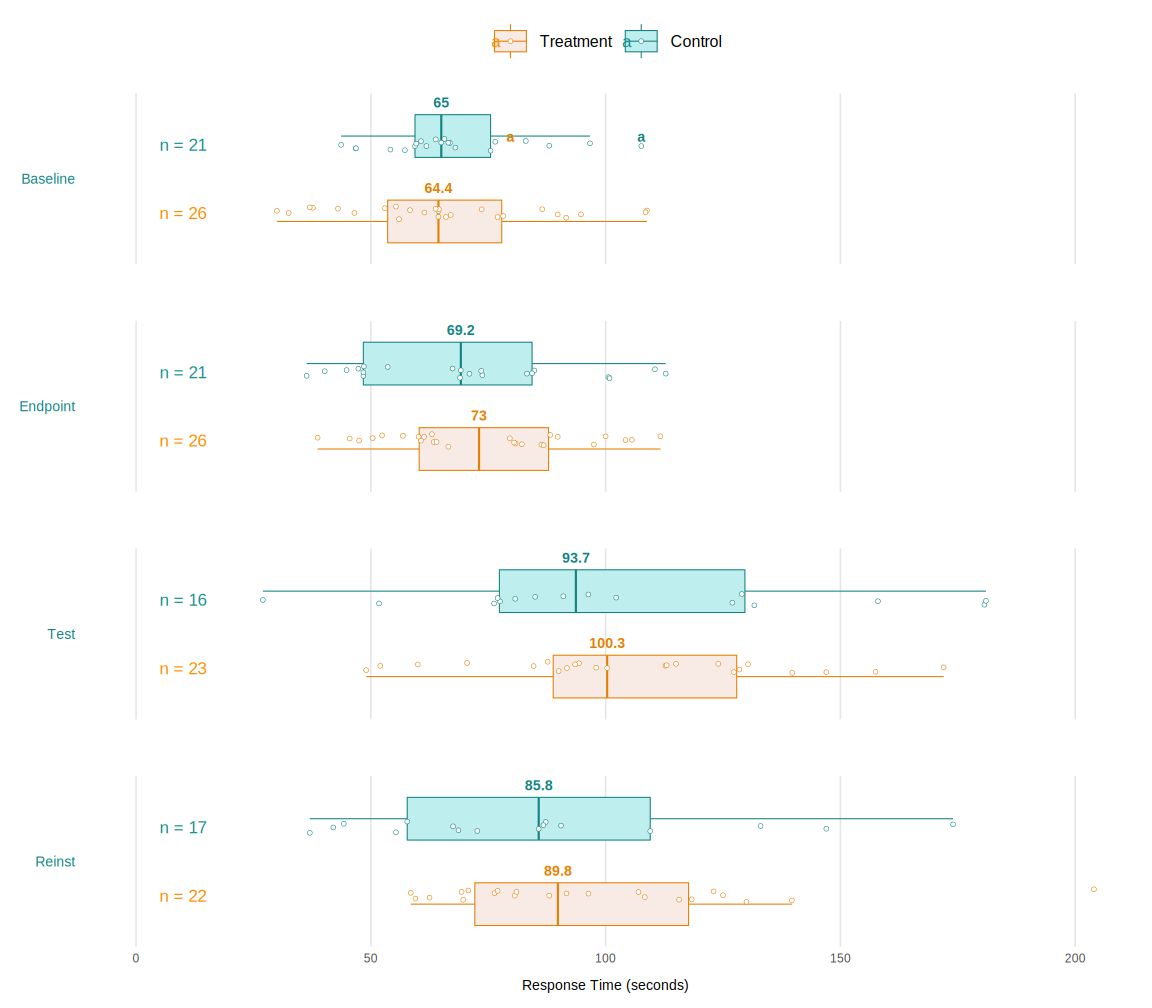
\includegraphics[keepaspectratio]{Francis_Masters_Thesis_files/figure-pdf/fig-decision-time-1.png}}
\end{center}

{\noindent \emph{Note.} Time taken to make a response across phases and
between conditions. Vertical lines show the median values. Boxes
represent the inter-quartile range (IQR), with whiskers extending out
1.5 times the IQR.}

\end{figure}

The decision latency data were analysed with a linear mixed-effects
model using the lme4 package for R
(\citeproc{ref-bates_fitting_2015}{Bates et al., 2015}). The model
included fixed effects of condition, time point, and an interaction
term. Subject ID was set as a random effect to account for repeated
measures. The decision time data were log-transformed. Type III ANOVA
was conducted using the car package (\citeproc{ref-fox_r_2019}{Fox \&
Weisberg, 2019}) to test for statistical significance of the fixed
effects. Pairwise comparisons with a Bonferroni correction were carried
out using the emmeans package in R
(\citeproc{ref-lenth_emmeans_2024}{Lenth, 2024}).

The ANOVA results revealed a significant effect of time (χ2 (3) = 24,
\emph{p} \textless{} .001), but failed to show a significant effect of
condition (χ2 (1) = 0.266, \emph{p} = .606). No time*condition
interaction effect was found (χ2 (3) = 1.88, \emph{p} = .598).

Post-hoc pairwise comparisons were carried out using estimated marginal
means with Bonferroni corrections applied to account for multiple
comparisons. Comparisons looked at within group differences in decision
latency across the four phases and also looked at between group
differences at each phase. The results indicated that there were two
within-group differences for the control subjects: test differed
significantly from baseline (\emph{d} = .56, \emph{p} \textless{} .001)
and test different significantly from endpoint (\emph{d} = .54, \emph{p}
\textless{} .001). There were four within-group differences for the
treatment subjects: test differed significantly from baseline (\emph{d}
= .85, \emph{p} \textless{} .001), reinstatement differed significantly
from baseline (\emph{d} = .67, \emph{p} \textless{} .001), test differed
significantly from endpoint (\emph{d} = .53, \emph{p} \textless{} .001),
and reinstatement differed significantly from endpoint (\emph{d} = .40,
\emph{p} = .007). There were no significant differences between groups.

The decision latency data do not support our hypothesis. Instead of
decision latency decreasing for the treatment group between baseline and
the end of conditioning as predicted, there was no change for either
treatment or control groups. Moreover, both groups showed increased
latency for decision making when comparing test to baseline. As a
caveat, it was noticed that planaria became smaller during the
experiment. This occurs when planaria have been deprived of food for
prolonged periods and is thought to be an evolved survival mechanism in
planaria
(\citeproc{ref-pascual-carreras_planarian_2020}{Pascual-Carreras et al.,
2020}; \citeproc{ref-thommen_body_2019}{Thommen et al., 2019}).
Interestingly, some research suggests that planarian locomotor velocity
is not correlated with body size
(\citeproc{ref-raffa_quantitative_2001}{Raffa et al., 2001}). But this
may only hold for between subjects comparisons during short experiments
but not within subject comparisons.

The change in body size that was observed throughout the experiment is
likely a sign of impaired health and low energy availability. One cause
of poor health may have been the repeated handling with a paintbrush,
which was suspected to have resulted in the death of several subjects.
While the remaining subjects could still complete the maze, their
movement may have been impaired from bodily damage. This would have
obscured any effect of increased motivation. These results were thus
compatible with at least three interpretations. One possibility is that
there was no increase in motivation among planaria. This hinders the
claim that the change in behaviour for treatment subjects was evidence
of learning. Another posibility is that response latency can measure a
change in motivation, but the effect of fatigue and injury in this case
impaired the ability to detect an increase. Finally, response latency
may simply not be a suitable measure of planarian motivation. Because of
the time and effort required to record response latency despite its
unknown validity, it was not measured during subsequent experiments.

\section{Experiment 3}\label{sec-experiment-3}

The y-maze experiment carried out in Experiment 2 suffered from several
procedural issues. First, the y-maze contained a divot at the end of the
runway that planaria would often swim into and circle around -- possibly
disturbing any sense of direction relative to the start of the maze.
Second, due to handling planaria with a paint brush, the death rate was
relatively high. Third, the number of trials where a subject failed to
respond was high, perhaps due to fatigue from too many trials per day
(\citeproc{ref-best_maze_1962}{Best \& Rubinstein, 1962};
\citeproc{ref-lee_conditioning_1963}{Lee, 1963}). Despite these
limitations, there was some indication that planaria were able to learn
and retain a conditioned response and that this may endure for at least
two weeks. While a replication of experiment 2 would have been
beneficial, due to time constraints we decided that the project would
progress and include a regeneration phase.

A third experiment was thus carried out which aimed to improve on the
limitations described for experiment 2 and test whether memories can be
retained through regeneration. Due to preliminary success by another
colleague in our lab who used methamphetamine to condition planaria,
this project also adopted methamphetamine as the reinforcing stimulus
(unpublished data, Inveterate Neuroscience Laboratory). Methamphetamine
is a psychoactive compound similar to cocaine in that it also increases
extracellular dopamine levels
(\citeproc{ref-desai_monoaminergic_2010}{Desai et al., 2010};
\citeproc{ref-kuczenski_hippocampus_1995}{Kuczenski et al., 1995}).
Methamphetamine has been established elsewhere as a rewarding stimulus
for planaria in models of addiction and withdrawal
(\citeproc{ref-kusayama_reinforcing_2000}{Kusayama \& Watanabe, 2000};
\citeproc{ref-raffa_-opioid_2008}{Raffa et al., 2008};
\citeproc{ref-sacavage_withdrawal-like_2008}{Sacavage et al., 2008}).

\subsubsection{Colony Maintenance and
Handling}\label{colony-maintenance-and-handling-2}

The planaria and colony maintenance protocols were similar to those
described in Experiment 2. The key differences were that the colony was
stored in a small plastic container and once experimental subjects had
been collected they were stored in a separate experimental room. This
room was dimly illuminated with red light during experimentation and
otherwise kept dark. Planaria were handled using a plastic transfer
pipette with the tip cut off.

\subsubsection{Materials and
Procedure}\label{sec-exp-3-materials-and-methods}

Forty-two planaria were used for this experiment, all assigned to the
methamphetamine treatment group. No control group was used\sidenote{\footnotesize It
  was important to establish weather an increase in active arm entries
  is stable over the conditioning period. To allow for a large number of
  treatment subjects to be included, no control group was run}. There
were four experimental stages: baseline, conditioning, retention test,
and reinstatement (see Figure~\ref{fig-exp3_timeline}). Planaria
completed three trials per day. There were two days for baseline, five
days for conditioning, and one day each for the retention test and
reinstatement procedure. During baseline and conditioning trials
multiple planaria were run concurrently in separate Y-mazes. Each maze
was filled with 2ml of planaria water which was shaken gently to evenly
distribute the water throughout the runway and arms. Planaria completed
three trials per day with an intertrial interval of approximately 120
minutes. At the start of a trial, planaria were transferred to the start
of the maze runway using a plastic transfer pipette with the tip cut
off. A timer was stared once each planarian was placed in its maze
runway. Planaria were given up to five minutes to enter one of the arms.
Once a planarian had entered an arm, the plug was inserted to stop
liquid moving between compartments, after which approximately 0.675ml
remained in each arm\sidenote{\footnotesize Measured by extracting and weighing the
  volume of distilled water trapped in each arm, assuming a density of
  1g/ml. Small deviations are inevitable, but this was the most common
  value seen during our tests}. A planarian was considered to have
entered the arm when the plug could be safely inserted without touching
the planarian.

\begin{figure}

\caption{\label{fig-exp3_timeline}Graphical timeline of Experiment 3}

\centering{

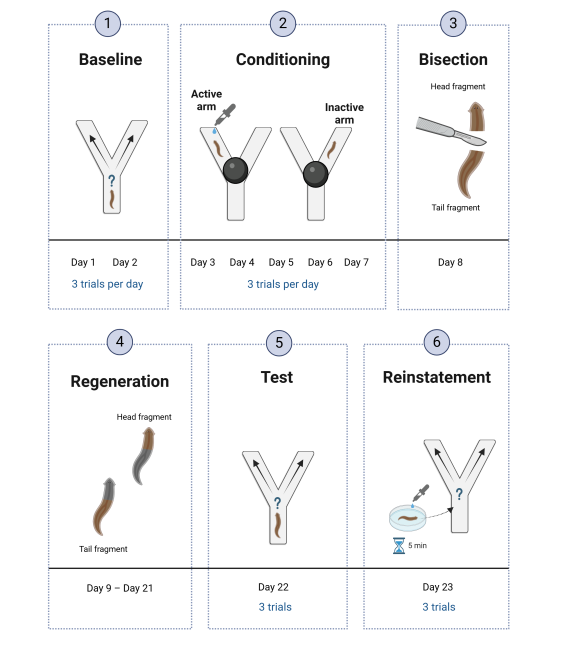
\includegraphics[width=1\linewidth,height=\textheight,keepaspectratio]{Francis_Masters_Thesis_files/figure-pdf/fig-exp3_timeline-1.png}

}

\end{figure}%

When treatment subjects entered the active arm, 29.35μL of
methamphetamine (in distilled water) was pipetted throughout the arm to
achieve a 10μM concentration. Nothing was added when planaria entered
the inactive arm. After an arm was chosen and, where applicable, the
drug was administered, the timer was restarted and three minutes were
given for absorption. The runway light was turned on after placing the
subject in the maze and turned off once the subject entered an arm. At
the end of each trial, planaria were washed thoroughly in a bath of
planaria water before being transferred back to their 12-well dish.
Mazes were rinsed and dried between each trial.

Planaria which exhibited evidence of learning at the end of conditioning
were bisected on the day following their last conditioning trail. For
the purposes of this experiment, a planarian was considered to have
learned if it entered the active arm on 4 or more out of the last 6
conditioning trials (\emph{n} = 10). For the bisection, planaria were
placed individually onto a plastic block with some planaria water and
cut transversely using a flat edge blade. The cut was made above the
pharynx and below the base of the head. This resulted in two subjects: a
tailless head fragment and a headless tail fragment. Planaria fragments
were placed into 12-well plates with labels to track the original
subject number and whether they were a head or tail fragment. Bisected
subjects were not fed for the duration of the experiment.

To enable sufficient time for regeneration of the head and tail
fragments, the memory retention test took place 14 days after bisection
(see Figure~\ref{fig-regeneration-timeline} for an example of the
regeneration process). For the memory retention test on day 14 of
regeneration, multiple planaria were run simultaneously in separate
y-mazes. Planaria were given five minutes to enter an arm. Once a
decision was made, the plug was inserted and planaria were left for
approximately 60 seconds before being moved back to the holding dish. No
additional liquid was added during test trials. The inter trial interval
was approximately 30 minutes. A reinstatement procedure was carried out
the following day. The reinstatement procedure was identical to the test
stage with the only additional step being drug exposure before each
trial. At the start of a run, planaria were placed into separate 4ml
solutions of planaria water containing 10μM of methamphetamine for five
minutes. At the end of the exposure interval, planaria were moved into
their separate Y-maze to begin the first trial.

Four improved 3D printed Y-mazes were used for this experiment (for
dimensions see Figure~\ref{fig-exp3_maze_dimensions}). Mazes were
printed using Siraya Tech professional UV resin. Similar to the mazes
used in Experiment 2, these mazes also contained an LED light embedded
in the resin after printing to induce negative phototaxis.

As described in Experiment 2, three exclusion criteria were used. The
exclusion criteria were: A) failing to complete at least four of the six
baseline trials; B) failing to complete at least two trials on
consecutive conditioning days; C) failing to complete at least four of
the last six trials of conditioning. None of the subjects were excluded
based on those criteria. No subjects died during the experiment.

\begin{figure}[!htbp]

{\caption{{Modified 3D printed
y-maze}{\label{fig-exp3\_maze\_dimensions}}}}

\begin{center}
\pandocbounded{\includegraphics[keepaspectratio]{Francis_Masters_Thesis_files/figure-pdf/fig-exp3_maze_dimensions-1.png}}
\end{center}

{\noindent \emph{Note.} Four Y-mazes (one pictured here) were printed
using Siraya Tech professional UV resin. A white LED was drilled into
the resin at the start of the runway to induce negative phototaxis. The
light was powered by a single 9V battery. A silicone plug was molded to
block liquid transfer after a planarian entered one of the arms.}

\end{figure}

\begin{figure}[!htbp]

{\caption{{Planaria regeneration
timeline}{\label{fig-regeneration-timeline}}}}

\begin{center}
\pandocbounded{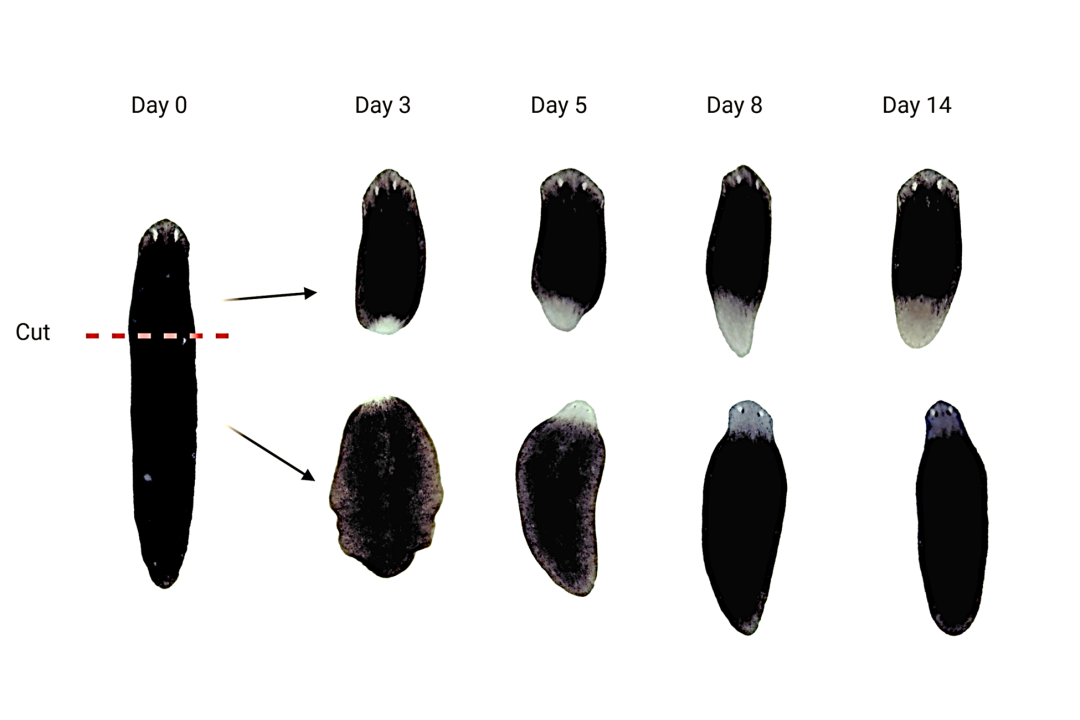
\includegraphics[keepaspectratio]{Francis_Masters_Thesis_files/figure-pdf/fig-regeneration-timeline-1.png}}
\end{center}

{\noindent \emph{Note.} The image above shows the regeneration process
for one of the experimental subjects used in this project. Soon after
bisection, a blastema containing stem cells appears at the wound site
which gives it the white colouring. The contrast and sharpness of the
planaria have been adjusted to make the regenerating section more
visible. The regeneration process has been described in detail by
Reddien and Alvarado (2004).}

\end{figure}

\subsubsection{Results and Discussion}\label{sec-results-and-discussion}

The majority of subjects had an initial preference towards the right arm
(\emph{n} = 22), with just over a quarter favouring the left arm
(\emph{n} = 13) and a few having no preference (\emph{n} = 7). This
experiment employed a biased design so that the active arm to be
reinforced was the opposite of the initial preference or randomly
assigned for those with no initial preference. The left arm was active
for 25 subjects, and the right arm was active for 17 subjects.

Figure~\ref{fig-Exp4_conditioning_results_panel}A shows the change in
active arm preference across conditioning days for all subjects
(\emph{n} = 42). There was an increase in active arm entries which was
visible on the first day of conditioning. This change persisted over the
five conditioning days, although there was a slight downward trend as
conditioning proceeded. A paired t-test was used to test whether there
was a significant difference in the proportion of active arm entries
between baseline and endpoint. At the end of conditioning, planaria
entered the active arm significantly more often than before conditioning
(\emph{t}(41) = -4.53, \emph{d} = 0.7, \emph{p} \textless{} .001). This
change in preference between baseline and endpoint can be seen in
Figure~\ref{fig-Exp4_conditioning_results_panel}B.

Figure~\ref{fig-Exp4_conditioning_results_panel}C and D show the memory
retention and reinstatement data for bisected planaria (\emph{n} = 10)
that were given 14 days to regenerate. Paired t-tests were used to
assess whether the active arm preference after regeneration and during
reinstatement were significantly different from baseline. For the
post-regeneration memory test, we failed to find a difference between
the heads (\emph{t}(9) = 1.72, \emph{d} = 0.54, \emph{p} = .12) or tails
(\emph{t}(9) = 1.86, \emph{d} = 0.59, \emph{p} = .096) compared to the
baseline active arm entries. Similarly, the reinstatement results failed
to demonstrate a significant difference between the heads (\emph{t}(9) =
1.34, \emph{d} = 0.42, \emph{p} = .215) or tails (\emph{t}(9) = 0.67,
\emph{d} = 0.21, \emph{p} = .521) compared to the baseline active arm
entries.

\begin{figure}[!htbp]

{\caption{{Learning and Memory Retention Through Decapitation in Meth
Treated Planaria}{\label{fig-Exp4\_conditioning\_results\_panel}}}}

\begin{center}
\pandocbounded{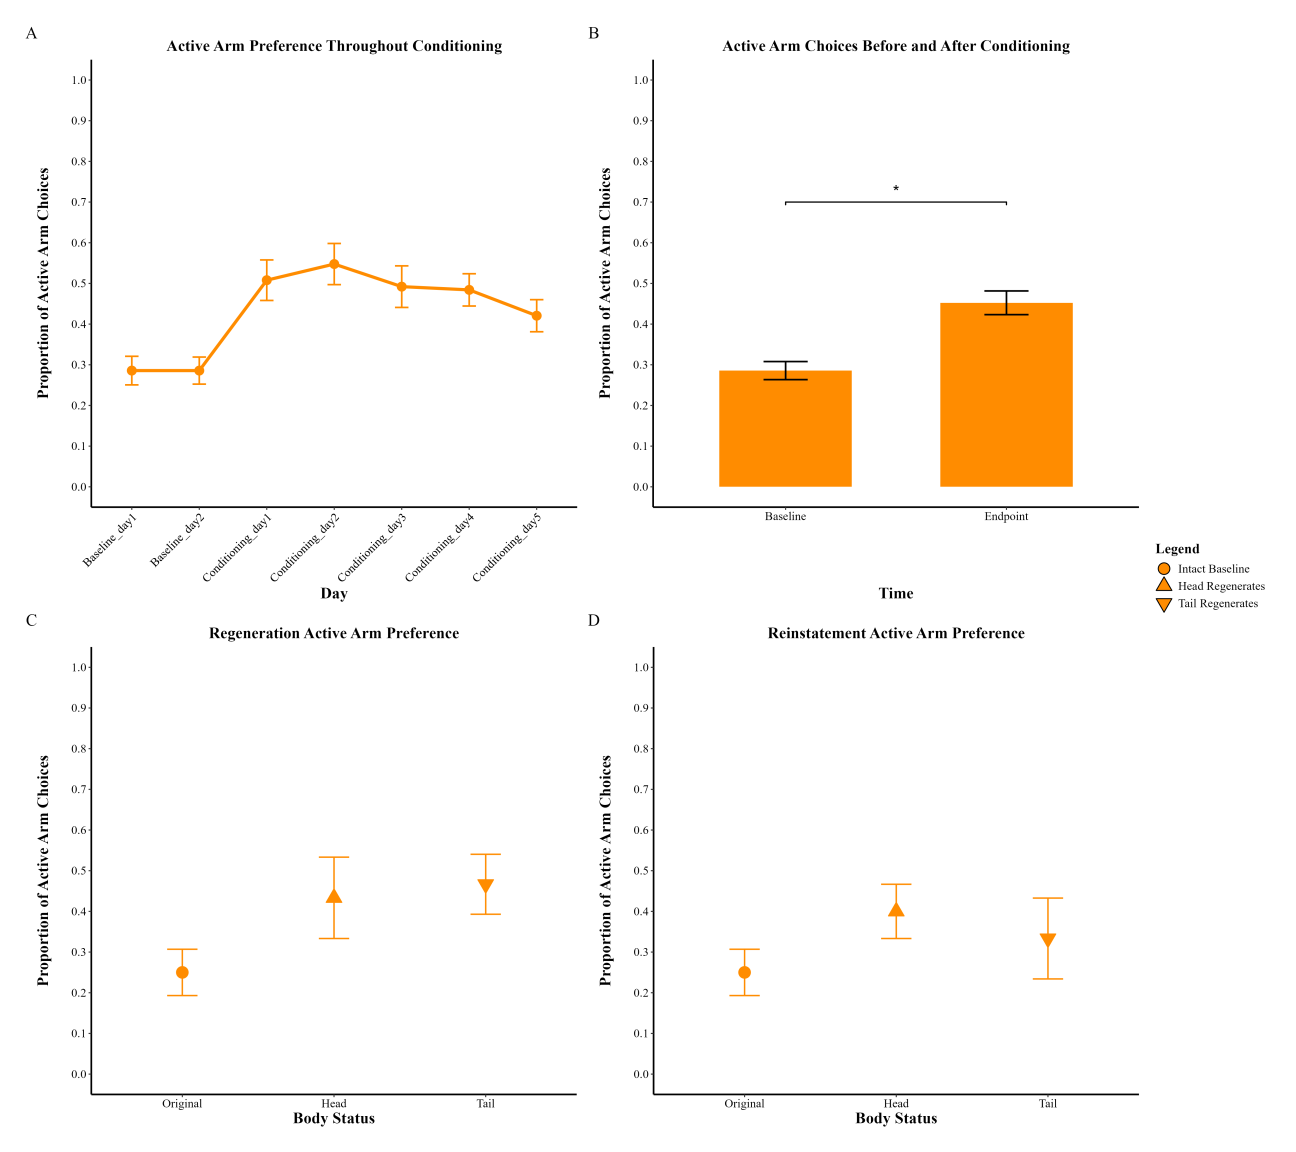
\includegraphics[keepaspectratio]{Francis_Masters_Thesis_files/figure-pdf/fig-Exp4_conditioning_results_panel-1.png}}
\end{center}

{\noindent \emph{Note.} Changes in Y-maze active arm preference across
experimental phases. The baseline phase included 6 trials, conditioning
endpoint included the final 6 trials of conditioning, and both test and
reinstatement phases included 3 trials each. A) shows the mean
proportion of active arm entries for baseline and conditioning. B)
Methamphetamine treated subjects showed a significant difference in
their active arm entries between baseline and endpoint. C) Despite a
visual trend showing greater active arm entries for regenerates compared
to baseline in the memory retention test, the patterns were not
significant. D) The reinstatement procedure failed to generate
significant differences in active arm entries compared to baseline.
Error bars represent standard error of the mean. * = p \textless.05}

\end{figure}

The results described provide preliminary evidence that methamphetamine
can be used to shape the behaviour of planaria in a Y-maze. The
behavioural change took place rapidly, with an increase in active arm
entries visible after one day of conditioning. The speed at which
behaviour change takes place is likely conditional on when planaria
sample the active arm. By chance, many subjects in one group may enter
the active arm on the first or second trial whereas in subsequent groups
it may take subjects three or four trials. While a gradual increase in
the active arm entries was expected, this rapid increase can be
explained by the fact that 22 subjects entered the active arm on the
first trial.

It could be argued that what appears to be a change in preference
towards the active arm (i.e., successful conditioning) is actually the
expression of truly random behaviour. Given a binary choice, if the
planaria were behaving randomly you would expect them to enter each arm
50\% of the time on average. Because the proportion of active arm
entries centered around 0.5 during conditioning, this could reasonably
explain the observed behaviour. In contrast, if the behaviour was
random, then we explain why the baseline level of active arm entries was
low across two consecutive conditioning days. If planaria do not
typically have a directional preference, we should have seen more
variation between day one and two during baseline. Moreover, as the
frequency of active arm entries did not return to baseline levels at all
throughout conditioning, we cannot easily attribute this pattern to
chance. As no control group was run, it is not clear whether a similar
pattern would occur without active reinforcement.

Although neither the head or tail regenerates differed significantly in
their active arm entries compared to baseline, the group means were all
visually higher compared to baseline (see
Figure~\ref{fig-Exp4_conditioning_results_panel} ). For example, the
proportion of active arm entries for tail regenerates (\emph{M} = 0.467)
was similar to what was seen at the end of conditioning for the original
sample (\emph{M} = 0.452). It must of course be noted that the failure
to find a significant effect despite the apparent trends may be due to
the small sample size for regenerates (\emph{n} = 10). Larger samples in
the future may help identify subtle effects if they in fact exist.
Nevertheless, the current data indicate that, although planaria can be
conditioned using a y-maze, there is no strong evidence that this
learned response survives bisection and regeneration. A stronger test of
the hypothesis in the future would require the inclusion of a control
group and larger sample sizes. Moreover, prior research suggests that
methamphetamine can increase the strength of learning in a dose
dependent manner (\citeproc{ref-kusayama_reinforcing_2000}{Kusayama \&
Watanabe, 2000}). It may therefore be beneficial to use a higher dose in
future experiments.

\section{Experiment 4}\label{sec-experiment-4}

The Y-maze experiment carried out in Experiment 3 made several
improvements on the materials and procedure from Experiment 2. Yet the
results were difficult to interpret due to a number of limitations.
Specifically, it did not employ a control group, a small number of
subjects were used for the regeneration tests, and the change in active
arm entries was significant but still relatively weak. To address these
limitations, this experiment included a control group, used more
subjects in the regeneration phase, and used a higher dose of
methamphetamine for reinforcement.

\subsubsection{Colony Maintenance and
Handling}\label{colony-maintenance-and-handling-3}

The planaria maintenance and handling protocols were identical to those
described in Experiment 3.

\subsubsection{Materials and Methods}\label{materials-and-methods}

This experiment used two groups: a treatment group (\emph{n} = 15) which
received methamphetamine and a control group (\emph{n} = 15) which
received vehicle only. There were four experimental stages: baseline,
conditioning, regeneration test, and reinstatement (see
Figure~\ref{fig-exp3_timeline}) . The materials and procedures used here
were the same as Experiment 3 except for the following modifications.
The active arm was reinforced with 58.7μL of methamphetamine (in
distilled water) to reach a final concentration of 20μM. Control
subjects received an equal volume of vehicle only (distilled water) when
they entered the active arm, and were otherwise treated the same as the
treatment subjects. At the end of conditioning, all subjects were
bisected into head and tail halves. For conditioning and testing
procedures, the intertrial intervals were approximately 90 minutes and
60 minutes, respectively. For the reinstatement phase, all regenerated
planaria, including control subjects, were bathed in 20μM
methamphetamine prior to each trial. The exclusion criteria exployed
were the same as in Experiment 2. None of the subjects used for this
experiment were excluded based on those criteria. No subjects died
during this experiment.

\subsubsection{Results and Discussion}\label{results-and-discussion-2}

There was a slight bias in baseline arm preference with 12 subjects
favouring the right arm, 9 favouring the left arm, and 9 having no
preference. This experiment employed a biased design such that the
active arm to be reinforced was the opposite of the initial preference
or randomly assigned for those with no initial preference. The left arm
was active for 15 subjects, and the right arm was active for 15
subjects.

Figure~\ref{fig-Exp7_conditioning_results_panel}A shows the proportion
of active arm entries throughout conditioning for both treatment
(\emph{n} = 15) and control (\emph{n} = 15) subjects. The treatment
group exhibits a steady increase in active arm entries over the first
three conditioning days. However, this begins to decrease sharply after
day three. The control group shows little variation across conditioning.
To assess whether the endpoint active arm preference differed from
baseline, a generalised linear mixed effects model with family set to
binomial was fitted in R using the lme4 package
(\citeproc{ref-bates_fitting_2015}{Bates et al., 2015}). Subject ID was
set as a random effect, with condition, time point and the interaction
term as fixed effects. The model analysed the proportion of entries into
the active arm out of six total trials at each time point. Pairwise
comparisons with a Bonferroni correction were carried out using the
emmeans package in R (\citeproc{ref-lenth_emmeans_2024}{Lenth, 2024}). A
Type III ANOVA was conducted using the car package
(\citeproc{ref-fox_r_2019}{Fox \& Weisberg, 2019}) to identify whether
there was a significant effect of condition or time, or an interaction
effect.

There was a significant main effect of time (χ²(1) = 7.179, \emph{p} =
.007). and a significant main effect of condition (χ²(1) = 5.021,
\emph{p} = .025). We did not detect a significant condition * time
interaction (χ²(1) = 0.16, \emph{p} = .689). Post-hoc pairwise
comparisons were carried out using estimated marginal means with a
Bonferroni corrections applied to account for multiple comparisons.
Comparisons looked at within group differences in response probability
over time and between group differences at each time point. The within
group comparison showed that endpoint was significantly higher compared
to baseline for treatment subjects only (OR = 0.51, \emph{z} = -2.23,
\emph{p} = .025). The post-hoc comparisons failed to show any
significant between-group differences at baseline or endpoint. This
indicates that while active arm entries were higher for the treatment
group overall, the individual data points were not significantly
different when comparing the treatment group to the control group.

Paired t-tests were used to determine whether there were significant
within group differences when comparing memory retention and
reinstatement data to baseline active arm entries (see
Figure~\ref{fig-Exp7_conditioning_results_panel} C and D). For the
initial memory retention test on day 14 the control heads differed
significantly from their baseline active arm preference (\emph{t}(14) =
3.31, \emph{d} = 0.85, \emph{p} = .005). Treatment heads differed
significantly from their baseline active arm preference (\emph{t}(14) =
4.07, \emph{d} = 1.05, \emph{p} = .001). Control tails differed
significantly from their baseline active arm preference (\emph{t}(14) =
2.24, \emph{d} = 0.34, \emph{p} = .042). For reinstatement on day 15, no
significant differences were found between heads or tails and their
respective baseline values for either group.

The data presented in Figure~\ref{fig-Exp7_conditioning_results_panel}
support the claim that methamphetamine can be used to successfully shape
the responses of planaria in a Y-maze. In particular,
Figure~\ref{fig-Exp7_conditioning_results_panel}A shows a gradual
increase in active arm selection for the treatment group across the
first three days of conditioning. Similar to the trend seen in
Experiment 3 (Figure~\ref{fig-Exp4_conditioning_results_panel}A),
treatment subjects exhibited a decrease in active arm entries towards
the end of conditioning. The control group showed little change in their
behaviour during conditioning.

\begin{figure}[!htbp]

{\caption{{Learning and Memory Retention Through Decapitation in
Planaria}{\label{fig-Exp7\_conditioning\_results\_panel}}}}

\begin{center}
\pandocbounded{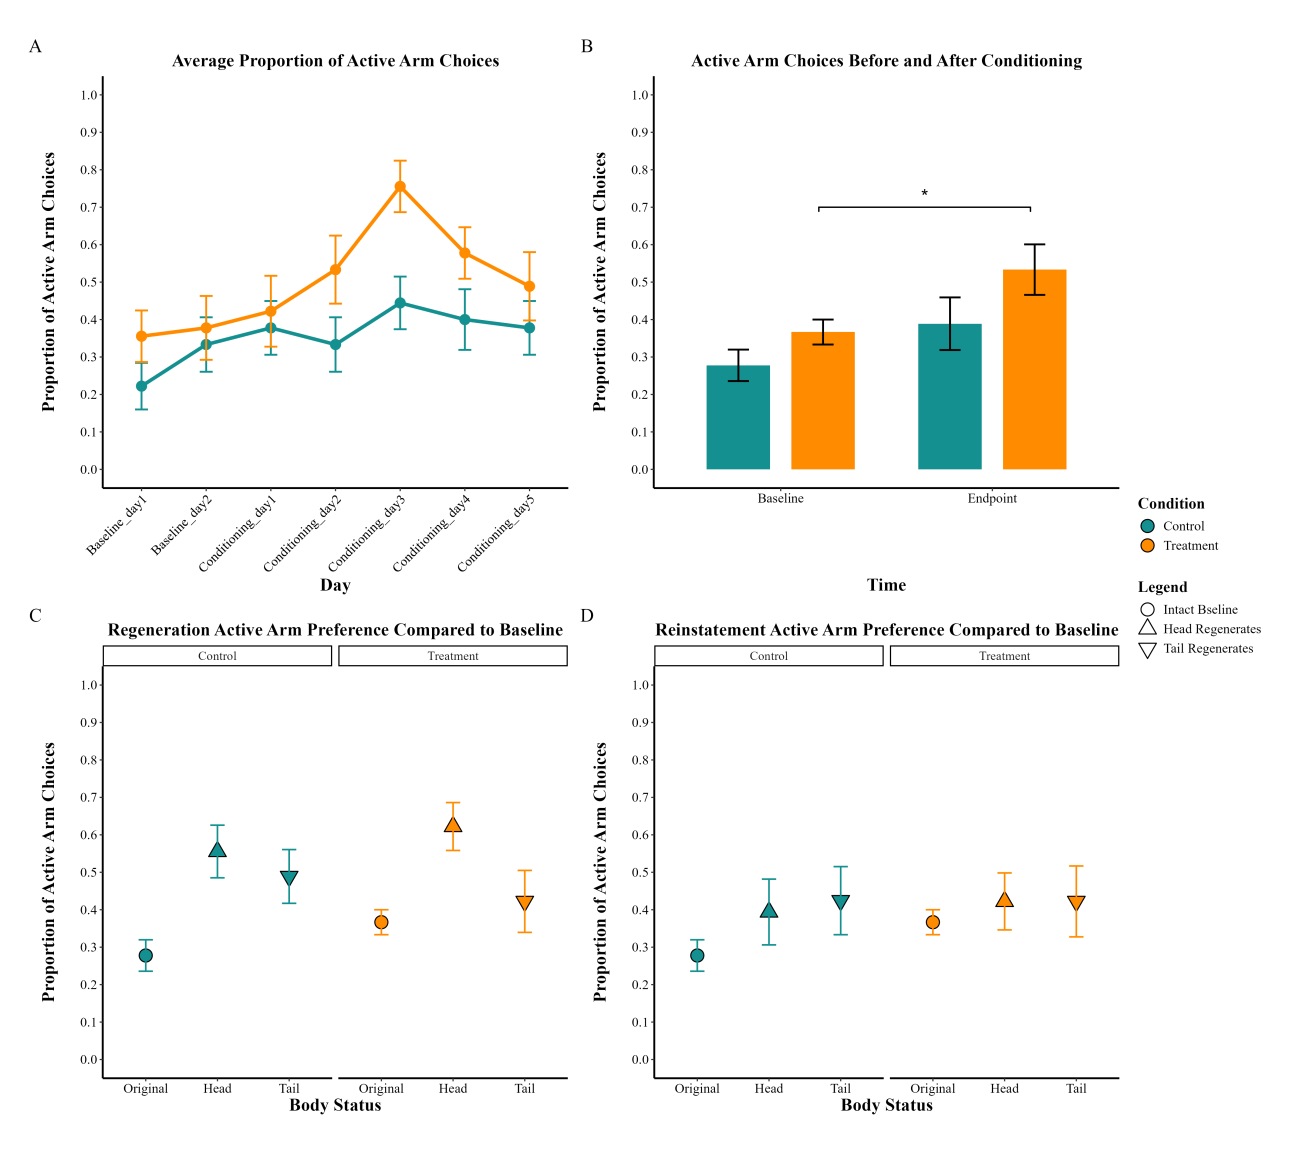
\includegraphics[keepaspectratio]{Francis_Masters_Thesis_files/figure-pdf/fig-Exp7_conditioning_results_panel-1.png}}
\end{center}

{\noindent \emph{Note.} Changes in Y-maze active arm preference across
experimental phases. The baseline phase included 6 trials, conditioning
endpoint included the final 6 trials of conditioning, and both test and
reinstatement phases included 3 trials each. A) shows the mean
proportion of active arm entries for baseline and conditioning for both
treatment and control subjects. B) Methamphetamine treated subjects
showed a significant difference in their active arm entries between
baseline and endpoint. No difference was found for control subjects. C)
The day 14 retention test found that control head and tail regenerates,
and treatment head regenerates differed significantly from baseline. D)
No significant differences were observed between regenerates of either
group and their respective baseline values during reinstatement. Error
bars represent standard error of the mean. * = p \textless.05}

\end{figure}

\section{Experiment 5}\label{sec-experiment-5}

The experiments described above support the claim that planaria can
obtain an operantly conditioned response. Yet, as can be seen from
Figure~\ref{fig-exp2decisions},
Figure~\ref{fig-Exp4_conditioning_results_panel} and
Figure~\ref{fig-Exp7_conditioning_results_panel}, the response was not
stable. The conditioned response tended to reach its peak early during
conditioning and then diminished towards baseline values despite still
being actively reinforced. It is not clear whether the reversion to
baseline behaviour is a sign of forgetting, drug tolerance, or active
rejection of a reinforced direction (described in
\citeproc{ref-best_maze_1962}{Best \& Rubinstein, 1962, pp. 565--566}).
To properly test memory retention through regeneration, it is important
to have a high rate of successful responses just prior to bisection.
Otherwise, what appears to be a lack of retention in regenerates may
just be a continuation of an already declining response rate. An
additional Y-maze experiment was therefore carried out.

Rather than having a pre-determined conditioning period, it was decided
that data would be inspected each day for evidence of learning. A mean
proportion of active arm entries above 0.6 for the treatment group would
trigger an end of the conditioning period. This was to ensure the active
arm was preferred by planaria so as to give the greatest chance of
retaining the learned response throughout the regeneration period.
Initiation of the regeneration phase was thus conditional on whether
adequate learning was shown for the treatment subjects.

\subsubsection{Colony Maintenance and
Handling}\label{colony-maintenance-and-handling-4}

The planaria maintenance and handling protocols were identical to those
described in Experiment 3.

\subsubsection{Materials and Procedure}\label{materials-and-procedure-1}

This experiment used two groups: a methamphetamine treated group
(\emph{n} = 24) and a control group (\emph{n} = 24) which received
vehicle only. This experiment had two stages: baseline and
conditioning\sidenote{\footnotesize The treatment subjects failed to show adequate
  evidence of learning. Given the failure of learning and the extended
  time required to perform the regeneration phase, it was decided that
  the experiment would be terminated after day four of conditioning.}.
The materials and procedures used here for baseline and conditioning
were identical to those in Experiment 4. The exclusion criteria employed
were the same as in Experiment 2. None of the subjects used for this
experiment were excluded based on those criteria. No subjects died
during the experiment.

The mean proportion of active arm entries for treatment and control
subjects were monitored each day. The data were graphed to show daily
active arm entries compared to baseline. No statistical analyses were
performed during the conditioning period. After day four of conditioning
the experiment was stopped due to a consistent decrease in active arm
entries among the treatment group.

\subsubsection{Results and Discussion}\label{results-and-discussion-3}

An approximately equal number of subjects preferred the right arm
(\emph{n} = 20) and left arm (\emph{n} = 21), with a small number of
subjects having no preference (\emph{n} = 7) at baseline. This
experiment employed a biased design, such that the active arm to be
reinforced was the opposite of the initial preference, or randomly
assigned for those with no initial preference. The left arm was active
for 23 subjects, and the right arm was active for 25 subjects.

Figure~\ref{fig-Exp8_conditioning_results_panel}A shows the change in
active arm preference across conditioning days for both treatment
(\emph{n} = 24) and control (\emph{n} = 24) subjects. The treatment
group demonstrates a sudden jump on the first day of conditioning. This
change remains stable for one day before declining towards baseline. The
control group shows a steady increase across days, with a slight
decrease on the last day of conditioning. To assess whether the endpoint
active arm preference differed from baseline, a generalised linear mixed
effects model with family set to binomial was fitted in R using the lme4
package (\citeproc{ref-bates_fitting_2015}{Bates et al., 2015}). Subject
ID was set as a random effect, with condition, time point and the
interaction term as fixed effects. The model analysed the proportion of
entries into the active arm out of six total trials at each time point.
Pairwise comparisons with a Bonferroni correction were carried out using
the emmeans package in R (\citeproc{ref-lenth_emmeans_2024}{Lenth,
2024}). A Type III ANOVA was conducted using the car package
(\citeproc{ref-fox_r_2019}{Fox \& Weisberg, 2019}) to identify whether
there was a significant effect of condition or time, or an interaction
effect.

There was a significant main effect of time (χ²(1) = 15.511, \emph{p}
\textless{} .001), but no significant effect of condition or a time *
condition interaction. Post-hoc pairwise comparisons compared the
proportion of arm entries at baseline to endpoint. After four days of
conditioning with 20μM of methamphetamine, treatment subjects were
significantly more likely to enter the active arm (OR = 1.69, \emph{z} =
2.04, \emph{p} = . 042) compared to baseline. After four days of
conditioning with vehicle only, control subjects were significantly more
likely to enter the active arm (OR = 2.48, \emph{z} = 3.55, \emph{p}
\textless{} .001) compared to baseline. We did not detect any
significant between-group differences.

The results presented here conflict with those presented in Experiment
4. As can be seen in Figure~\ref{fig-Exp7_conditioning_results_panel},
the active arm preference for the control group did not shift
significantly, suggesting that in Experiment 4, the change observed in
the treatment group was due to reinforcement with methamphetamine.
However, the results presented here show a large shift in the control
groups behaviour despite being treated with vehicle only. Further still,
the control group appears to have experienced a greater shift in their
preference than the treatment group (albeit the between groups
comparison at endpoint was not statistically significant). What appeared
to be effective conditioning as a result of methamphetamine
administration in Experiment 4 may instead be the result of some other
extraneous other variable. Or, as described earlier, it may indicate
that planaria do not typically have a directional preference in the
Y-maze.

\begin{figure}[!htbp]

{\caption{{Failure to Find Evidence of Learning Among Meth Exposed
Planaria}{\label{fig-Exp8\_conditioning\_results\_panel}}}}

\begin{center}
\pandocbounded{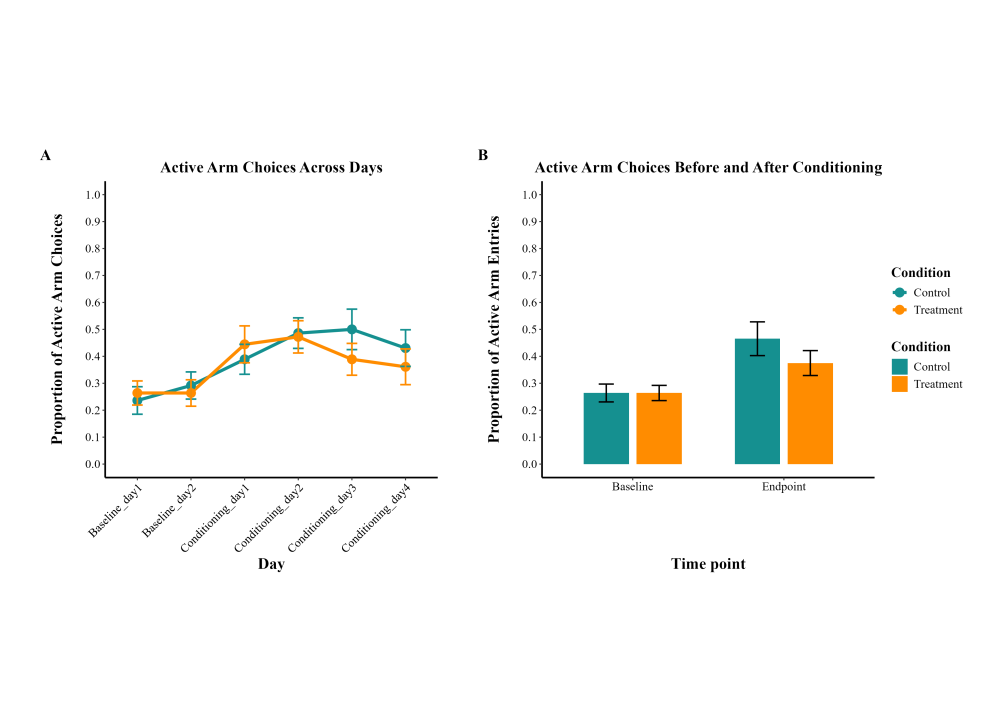
\includegraphics[keepaspectratio]{Francis_Masters_Thesis_files/figure-pdf/fig-Exp8_conditioning_results_panel-1.png}}
\end{center}

{\noindent \emph{Note.} Changes in Y-maze active arm preference across
experimental phases. The baseline phase included 6 trials, conditioning
endpoint included the final 6 trials of conditioning. A) shows the mean
proportion of active arm entries for baseline and conditioning. B) Both
methamphetamine treated subjects and control subjects treated with
vehicle only showed a significant difference in their active arm entries
between baseline and endpoint. Error bars represent standard error of
the mean.}

\end{figure}

\newpage

\section{Discussion}\label{sec-discussion}

\subsection{Review of Findings}\label{sec-review-of-findings}

Planaria have gained attraction as a model organism in several areas of
science ranging from drug addiction to limb regeneration. But it must be
said that the most interesting aspect of planaria research involves the
study of memory retention through decapitation and head regeneration.
Despite a pockmarked past in the 20th century, recent experiments
suggest that, even after losing their brain, planaria can maintain
previously acquired associative memories which can then be acted upon
once a new brain is regenerated
(\citeproc{ref-samuel_addiction-related_2021}{Samuel et al., 2021};
\citeproc{ref-shomrat_automated_2013}{Shomrat \& Levin, 2013}).

While this phenomenon is extraordinary in and of itself, whether it has
implications for the kinds of memories that concern humans has not yet
been shown. For example, prior experiments have focused on things like
familiarity with a surface texture and other simple associative
memories. There have been no clear tests for persistence of complex
forms of memories formed through operant conditioning. Just as humans
must navigate through the world to accomplish their goals (e.g., getting
to work on time), operant conditioning requires that a subject learns
that it must maneuver its body through the environment in a particular
way to receive a reward.

A number of factors may explain the lack of research concerning whether
operantly conditioned responses survive decapitation and brain
regeneration. For example, researchers may have tried and failed to
achieve successful conditioning with operant procedures. While planaria
are incredibly capable despite their rudimentary body plan,
reinforcement learning may fall outside of their cognitive capability.
Alternatively, it may be within the scope of planarian capability but
cannot be reliably induced. Just as some humans excel in intellectual
activities while others struggle. Planaria too may exhibit high
variability in their cognitive capacities.

Another possible explanation for this research gap is the demanding
schedule operant conditioning imposes on experimenters. Classical
conditioning methods such as CPP often require a brief set up but then
have periods of idle time while the subject is exposed to an
environmental condition, with software allowing for automatic tracking
of movement. Operant conditioning, on the other hand, typically requires
continuous observation of the subject to ensure a reward is delivered
reliably and in close proximity to the performance of the desired
behaviour. When taking into account the necessary sample size and number
of observations required per subject, this amounts to a large time
commitment.

The present research aimed to plug this gap in the planarian learning
and memory literature. Specifically, it aimed to identify whether the
phenomena of memory retention through decapitation and regeneration in
planaria could be extended to more complex forms of memory.
Additionally, it investigated whether time-dependent forgetting can be
reversed with a reinstatement procedure.

As a preliminary step, in Experiment 2 we investigated whether a Y-maze
can be used to induce a conditioned response and whether this can
persist for at least two weeks -- the approximate period required for
regeneration of planaria. Although both cocaine treated and control
subjects entered the active arm more frequently at the end of
conditioning, only the cocaine treated group showed evidence of a
persistent change in behaviour when tested two weeks later. During the
reinstatement procedure the following day, not only did reinstatement
fail to reinstate or increase memory strength among the cocaine treated
group, but the cocaine treated groups behaviour actually returned to
baseline levels. This suggests the learned response which persisted for
two weeks in the cocaine treated group was rapidly extinguished across
three trials during the memory retention test. This observation of rapid
extinction is consistent with the findings of Amaning-Kwarteng et al.
(\citeproc{ref-amaning-kwarteng_relapse_2017}{2017}) who observed
extinction over three trials in a CPP procedure. Moreover, recent work
in our lab suggests conditioned responses in the Y-maze are extinguished
quickly if not reinforced (unpublished data, Invertebrate Neuroscience
Lab). Contrary to expectations, the time taken to make a decision did
not improve for the treatment group.

Over a series of experiments we then tested whether an operantly
conditioned response can survive bisection and regeneration. Despite a
visual trend in Experiment 3 which appeared to show memory retention
through regeneration, we failed to find evidence of significant memory
retention in regenerates. These results were followed up in Experiment 4
with a larger sample size. We found evidence of memory retention after
regeneration in the head regenerates of treatment subjects.
Surprisingly, the control group (treated with vehicle only) also showed
evidence of a change in behaviour after regeneration. That is, despite
showing no statistically significant shift in behaviour during
conditioning, the regenerated heads and tails of control subjects showed
a high proportion of active arm entries after regeneration.

Although Experiment 3 and 4 implied successful conditioning of drug
treated subjects, Experiment 5 failed to demonstrate adequate evidence
of learning in the treatment group. Furthermore, the control group in
Experiment 5 showed a significant shift in their behaviour. This shift
was comparable in size to that observed among methamphetamine treated
subjects from Experiments 3 and 4. It is apparent that each of the
experiments described here, if inspected in isolation, would tell a
different story.

Having briefly summarised the findings at the level of each experiment,
we will now move to a general discussion of whether planaria can learn
an operantly conditioned response in a Y-maze. It is tempting to take
the observed shift in active arm preference for treatment subjects
across several experiments as evidence that we can successfully shape
planarian behaviour. However, in Experiment 2 and 5 we also found a
significant shift in the active arm preference of control subjects. A
change in the behaviour of drug exposed subjects can be interpreted as
successful reinforcement learning. But a change in the behaviour of
control subjects is more difficult to understand, especially when it
resembles a smooth learning curve.

It is possible that when control subjects received distilled water in
the active arm, the movement of liquid may have been experienced as a
positive stimulus and thus reinforced the responding of control
planaria. There is some evidence dating back more than a century that
planaria will actively swim against a current
(\citeproc{ref-allen_reversibility_1915}{Allen, 1915}) which suggests
moving water is preferred to still water. In partial support of this, it
was observed throughout the project that when the water in the planarian
housing was changed, planaria became more motile. However, whether this
represents approach or avoidance behaviour is unknown.

In all cases where planaria became more likely to enter the active arm,
be it for drug treated or control subjects, the proportion of active arm
entries floated around 0.5. While one interpretation holds that this is
evidence of learning in the treatment groups, an alternative explanation
is that planaria were exhibiting truly random behaviour. On this view,
the apparent baseline preference was the consequence of observing a
small number of trials. The bias that results from under sampling can be
illustrated by a simple example such as flipping a coin. Using a simple
unbiased coin flipping script in R, when we observed six coin flips per
trials, four repeated trials produced the following outcomes outcomes:
5:1, 3:3, 6:0 and 4:2 (ratio of tails to heads). Meanwhile, observing
100,000 coin flips in a single trial resulted in 49.6\% of the flips
being tails and 50.4\% being heads. Provided enough observations are
made, the stochastic nature of the variable is revealed. That our
apparent biases at baseline may simply be under sampling of a random
variable is supported by the results of Abbott and Wong
(\citeproc{ref-abbott_conditioning_2008}{2008}) who found that when
looking at a single baseline session containing ten trials, most
planaria showed arm preferences in a Y-maze procedure. However, when
combining thirty baseline trials across three days, most planaria showed
no arm preference.

If Abbott and Wong (\citeproc{ref-abbott_conditioning_2008}{2008}) are
correct in claiming that planaria typically do not have an arm
preference, we still need to explain why the proportion of active arm
entries observed in our experiments were consistent across two separate
baseline days. If the behavior was truly random, one would expect
greater variability between baseline day one and baseline day two.
However, across experiments for both treatment and control groups, the
proportion of entries into the active arm was approximately 0.3 on two
consecutive baseline days.

Although the planaria used by Abbott and Wong
(\citeproc{ref-abbott_conditioning_2008}{2008}) may not exhibit a
directional preference, given many documented behavioural differences
among planaria species
(\citeproc{ref-cochet-escartin_scrunching_2015}{Cochet-Escartin et al.,
2015}; \citeproc{ref-debold_differences_1965}{DeBold et al., 1965};
\citeproc{ref-mueller_use_2002}{Mueller \& Levin, 2002};
\citeproc{ref-samuel_addiction-related_2021}{Samuel et al., 2021}), it
may be that there are also differences in directional preferences.
Perhaps the species used throughout this project differed in their
behaviour from the Dugesia Tigrina used by Abbott and Wong
(\citeproc{ref-abbott_conditioning_2008}{2008}). A targeted
investigation is required to determine if the species of planaria used
here exhibit a directional bias in the Y-maze.

Moving now to the behaviour of control subjects, it is difficult to know
whether such dramatic shifts in behaviour are expected because there are
few studies available for comparison. The modern literature on planaria
behaviour in general conveys stable behaviour of the control group in
paradigms such as CPP
(\citeproc{ref-hutchinson_persistent_2015}{Hutchinson et al., 2015};
\citeproc{ref-jordan_conditioned_2023}{Jordan et al., 2023}). However,
early planaria conditioning work by Corning
(\citeproc{ref-corning_retention_1966}{1966}) exhibited a similar level
of variability of directional preference in a T-maze paradigm. In fact,
the control group in Corning
(\citeproc{ref-corning_retention_1966}{1966}) demonstrated a noticeable
increase in active arm preference across the first ten trials, with the
active arm preference remaining between 0.45 and 0.5 for the remaining
70 trials. In the case of Corning
(\citeproc{ref-corning_retention_1966}{1966}), despite this increase for
the control group, the treatment groups entered the active arm between
60--65\% of the time. In line with our observations from Experiment 3,
Corning (\citeproc{ref-corning_retention_1966}{1966}) saw a spike in
active arm entries for treatment subjects within the first ten trials.

Two recent projects which aimed to shape directional preferences also
found high variability among the control group. Read
(\citeproc{ref-read_reinforcing_2021}{2021}) observed that the
percentage of entries into the active arm varied from
\textasciitilde25\% at baseline to \textasciitilde50\% at the end of
conditioning for the control group. Another investigation (unpublished
data, Canales Laboratory) observed similar variation in active arm
entries when subjects were treated with cocaine alongside compounds
known to prevent cocaine seeking in rodents. All groups experienced a
large jump in active arm entries on the first day of conditioning,
hovering around 50\% and then declining towards baseline levels. This
resembles the behaviour seen in the control group within the current
project and, to some extent, matches the decline in active arm entries
seen in the treatment groups.

The intertrial interval is one factor that may affect the extent of
learning among planaria. It has been suggested elsewhere that planaria
learn mazes most effectively when a 30-minute intertrial interval is
used (\citeproc{ref-warren_comparative_1965}{Warren, 1965, p. 100}).
Moreover, larger intertrial intervals have been reported to mitigate the
effects of fatigue from repeated
trials(\citeproc{ref-best_maze_1962}{Best \& Rubinstein, 1962};
\citeproc{ref-lee_conditioning_1963}{Lee, 1963}). But the optimal
intertrial interval may differ largely between tasks. Some classical
conditioning procedures have had success when using an intertrial
interval of one minute. Crawford et al.
(\citeproc{ref-crawford_distribution_1966}{1966}) found that spaced
trials (at least one minute between) were more effective than massed
trials (only 30 seconds between).

The experiments employed here varied in their intertrial intervals.
Experiment two had a shorter intertrial interval of 15 minutes, while
the remaining experiments had intertrial intervals of 60 minutes or
more. This was due to a change in procedure. In Experiment 2, six
planaria were moved into temporary petri dishes and completed all of
their trials before the next group of six started their first trial.
Whereas in later experiments, planaria were taken straight from their
12-well housing compartments, with each planaria completing their first
trial before any planaria started their second trial. Although the
intertrial interval may play a role in the rate and extent of learning,
we did not observe any obvious difference based on this.

Another factor which may impact the rate of learning is the drug
concentration used. Across the experiments reported here, doses of
either 10μM or 20μM were administered. While these are similar to those
used in most studies of learning and addiction-like behaviour in
planaria (\citeproc{ref-amaning-kwarteng_relapse_2017}{Amaning-Kwarteng
et al., 2017}; \citeproc{ref-hutchinson_persistent_2015}{Hutchinson et
al., 2015}; \citeproc{ref-nayak_benzodiazepine_2016}{Nayak et al.,
2016}; \citeproc{ref-raffa_subadditive_2006}{Raffa et al., 2006};
\citeproc{ref-sacavage_withdrawal-like_2008}{Sacavage et al., 2008};
\citeproc{ref-turel_planaria_2022}{Turel, 2022}), there are a several
papers which have employed drug concentrations as high as 80μM with
success (\citeproc{ref-raffa_cocaine_2005}{Raffa et al., 2005};
\citeproc{ref-raffa_description_2005}{Raffa \& Desai, 2005};
\citeproc{ref-rawls_nitric_2006}{Rawls, Rodriguez, et al., 2006};
\citeproc{ref-umeda_cocaine_2004}{Umeda et al., 2004}).

As was observed in the dose-response analysis shown in
Figure~\ref{fig-boxplot}, there was no evidence that the doses 10μM or
20μM of cocaine affected planaria motility. We specifically sought out a
concentration that would not affect the movement of planaria during
subsequent trials. But a lack of physical effects may also indicate that
the drug is failing to have any psychoactive (and therefore rewarding)
effects for the planaria. Although higher concentrations may reduce the
speed with which planaria complete the Y-maze and increase the rate of
non-responses, it may also increase the strength of learning on average.
That said, some experiments have shown successful learning with drug
concentrations as low as 1μM
(\citeproc{ref-hutchinson_persistent_2015}{Hutchinson et al., 2015};
\citeproc{ref-vouga_stereochemistry_2015}{Vouga et al., 2015}). It would
thus be beneficial to systematically manipulate drug concentrations to
identify the optimal dose which maximises learning in the planaria
species used here.

Given the instability of planarian behaviour observed here, it is
difficult to recommend the Y-maze procedure as a viable conditioning
paradigm for the field. If the phenomena of memory retention through
regeneration is a reliable effect as is suggested by the literature
(\citeproc{ref-corning_retention_1966}{Corning, 1966};
\citeproc{ref-mcconnell_effects_1959}{McConnell et al., 1959};
\citeproc{ref-mueller_use_2002}{Mueller \& Levin, 2002};
\citeproc{ref-rhodes_effects_2024}{Rhodes \& Vierick, 2024};
\citeproc{ref-samuel_addiction-related_2021}{Samuel et al., 2021};
\citeproc{ref-shimojo_preservation_2022}{Shimojo et al., 2022};
\citeproc{ref-shomrat_automated_2013}{Shomrat \& Levin, 2013}),
understanding whether this extends to complex forms of memory is a
worthwhile pursuit. But to achieve this, a reliable method for
effectively shaping planaria behaviour is needed. The Y-maze procedure
may not be a reliable method. Instead, alternative operant conditioning
procedures may be better suited to carry on this research project. There
are several alternative methods for conditioning planarian. Some date
back to the early 20th century such as the Van Oye maze (e.g.,
\citeproc{ref-van_oye_over_1920}{Oye, 1920}), while others have only
appeared in the last decade. For example, Chicas-Mosier and Abramson
(\citeproc{ref-chicas-mosier_new_2015}{2015}) established a method where
the directed movement of planaria is reinforced with water in a crescent
petri dish. Although independent replications of these methods are
needed to demonstrate their viability, they may hold more promise for
successfully shaping planaria behaviour.

One key insight evident from the work performed here is that the
behaviour of planaria is highly variable. As was seen when assessing
planaria motility during the dose response procedure, there was large
variability among all groups. Some planaria covered the diameter of the
dish just two or three times during the 15-minute recording interval,
while many others traveled a distance 20 times greater than the dish
diameter. Both of these extremes were observed across four of the five
groups. Regarding the Y-maze, there was high variability in active arm
entries over time even among the control group. Moreover, when we
observed an increased preference for the active arm among
methamphetamine treated subjects, this change was not stable and began
to diminish rapidly towards the end of conditioning.

Behavioural volatility may be a general characteristic of planarian
behaviour. There is evidence for between species variability when
undergoing conditioning (\citeproc{ref-mueller_use_2002}{Mueller \&
Levin, 2002}; \citeproc{ref-samuel_addiction-related_2021}{Samuel et
al., 2021}), and even within species differences to slight changes in
environmental conditions including light, vibrations, size of the
recording dish and more (\citeproc{ref-rejo_optimization_2023}{Rejo et
al., 2023}). If planarian behaviour exhibits high within-subject
variability, the probability of arriving at a reliable operant
conditioning procedure may be low.

We shall now turn to the more philosophically interesting capability
addressed within this project: the retention of a learned response
through bisection and regeneration. The standing synaptic trace theory
of memory would suggest that a memory can only be retained if the
synaptic connections which underpin it are maintained. This theory would
be challenged if a change in behaviour, such as a conditioned arm
preference, is conserved in the tail regenerates of trained planaria.
Our results showed that head regenerates of methamphetamine treated
subjects maintained an active arm preference that was significantly
higher than baseline. However, the tail regenerates failed to show
retention of the active arm preference. Surprisingly, a spontaneous
change in the behaviour of controls was seen in regenerated head and
tails.

The head regenerates of trained planaria should in theory contain most
of the original brain cells present during the conditioning procedure.
Because, as synaptic trace theory predicts, the original dendritic
spines that underpin the memory would not be affected by the bisection.
The head regenerates could therefore act on previously acquired
information. This aligns with the behaviour of head regenerates from
methamphetamine exposed planaria in Experiment 4. The tail regenerates
of methamphetamine treated planaria also confirm the predictions of
synaptic trace theory. These regenerates did not differ significantly
from baseline in their proportion of active arm entries. A proponent of
the synaptic trace theory would argue that the necessary neural
connections that underlay the memory were absent in the tail half and,
therefore, the information could not possibly persist in the tail
regenerates.

While the observed results for methamphetamine treated regenerates are
explainable by the prevailing synaptic trace theory, the behaviour of
control subjects is much harder to parse. The head and tail regenerates
of control planaria exhibited a significantly higher proportion of
active arm entries compared to baseline. That is, despite showing no
evidence of learning during conditioning, the arm preference of
regenerate controls shifted in both halves after bisection. Moreover,
the proportion of active arm entries in the head and tail regenerates of
control subjects centered around 0.5, reflecting the earlier concern
that planaria may not have a true directional preference. While it is
tempting to claim that methamphetamine treated head regenerates are
demonstrating retention of a learned behaviour, the observed data cannot
rule out that under sampling of a random behaviour at baseline is
responsible for the pattern, rather than successful learning.

That the directional preference of planaria in a Y-maze may be random is
supported by the findings of Akiyama et al.
(\citeproc{ref-akiyama_spontaneous_2015}{2015}). Akiyama et al.
(\citeproc{ref-akiyama_spontaneous_2015}{2015}) found that a commonly
observed phenomenon in planaria, whereby they prefer to be on the wall
of a dish rather than on the base of the dish, is in fact due to
spontaneous behaviours that increase the likelihood of ending up on the
wall. The authors devised several experiments to show that, absent any
alluring or noxious stimuli, planaria move straight ahead until they
reach a wall. Moreover, they demonstrated that planaria perform a
side-to-side movement of their head while swimming (``wigwag
movement''), and that it is this spontaneous behaviour which affects
their path of motion. What often appears to be an intentional wall
seeking behavior may in fact be the result of two spontaneous behaviours
-- forward movement and head wigwagging. People often describe planarian
wall preference as if it is an intentional survival strategy. But as
Akiyama et al. (\citeproc{ref-akiyama_spontaneous_2015}{2015}) suggest,
planarian behaviour may be less intentional than initially presumed. If
true, this supports the conclusion that planaria do not have a true
directional preference.

The handling technique used to transfer planaria may have contributed to
the apparent behaviour changes observed across experiments. Planaria
were typically transferred into the Y-maze using a plastic transfer
pipette. This method made it difficult to precisely control the starting
position at the beginning of each trial. On occasion, the planaria would
land close to or on a wall of the maze. While this did not guarantee
that the planarian would enter a particular arm, if their default motion
is to continue moving straight as suggested by Akiyama et al.
(\citeproc{ref-akiyama_spontaneous_2015}{2015}), it may have biased the
outcome. This aligns with the experimenter's observations, as planaria
seemed more likely to enter the arm corresponding to a wall it landed on
or was closest to when entering the maze runway. Given the experimenter
was right-handed, the discharge angle of planaria was typically biased
towards the left hand wall. While most planaria landed on the floor of
the maze runway, this may have increased the chance that planaria land
on the left wall and enter the left arm. Fortunately, there was no
evidence of a left-arm bias in planaria. In fact, when considering the
baseline behaviour in Experiment 3 and 4, we found that subjects tended
to enter the right arm more often at baseline. Experiment five showed no
bias.

We may have effectively shaped the behaviour of treatment subjects in
Experiment 3 and 4. But because the extent of learning was limited and
the responses were not stable, the experiments reported here can only be
considered a weak test of whether planaria can retain an operantly
conditioned response through regeneration. However, even if
\emph{operantly} shaped behaviours cannot survive decapitation and brain
regeneration, this does not subtract from the well replicated effect of
memory retention seen with simple \emph{classical} conditioning
paradigms (\citeproc{ref-corning_retention_1966}{Corning, 1966};
\citeproc{ref-mcconnell_effects_1959}{McConnell et al., 1959};
\citeproc{ref-rhodes_effects_2024}{Rhodes \& Vierick, 2024};
\citeproc{ref-samuel_addiction-related_2021}{Samuel et al., 2021};
\citeproc{ref-shimojo_preservation_2022}{Shimojo et al., 2022};
\citeproc{ref-shomrat_automated_2013}{Shomrat \& Levin, 2013}). Although
simple associative memories may be less interesting, there is no reason
to suspect that the underlying storage mechanism differs from that used
for more complex memories. Kandel
(\citeproc{ref-kandel_molecular_2001}{2001}) drove this point home when
reflecting that: ``Our research suggests that the cellular and molecular
strategies used in Aplysia for storing short- and long-term memory are
conserved in mammals and that the same molecular strategies are employed
in both implicit and explicit memory storage''

Although the exact molecular cascades differ between forms of memory,
both classical and operant learning are thought to be underwritten by
changes among synapses (\citeproc{ref-kandel_molecular_2001}{Kandel,
2001}). This implies that conditioned texture preferences should,
according to the synaptic trace theory, be physically realised through
synaptic connections and their associated weights. Consequently, given
the synapses are presumed to be absent in the tail halves after
bisection, tail regenerates should not retain the conditioned
preferences of the original subjects. However, texture preferences and
other associative memories can survive partial or complete loss of the
brain in invertebrates, as was discussed at length in the literature
review. This directly challenges the synaptic trace theory. While
associations between neurons are clearly important for our ability to
change our behaviour based on past experiences, are they really the site
of memory storage?

This project investigated the scope of memory persistence through
regeneration among planaria. Since a number of experiments failed to
show clear evidence of learning, the verdict is still out as to whether
complex operantly conditioned behaviours can survive regeneration.
Viewed in isolation, it would be easy to take these failures as indirect
support for the synaptic trace theory -- of course memories cannot be
retained if the substrate of their storage is removed. The wider
empirical evidence of retention through regeneration, however, demands
that we provide an explanation of how even simple associative
information can survive in the tail halves of planaria. That a
particular piece of exploratory work comes up empty handed should not
detract from the mounting evidence suggesting there is more to the story
of information storage in biological systems. Rather, any existing
studies showing planaria may learn and retain memories, be they complex
or simple, should spur us on in the search for other mechanisms that may
act as repositories or facilitators of memory storage. But what other
mechanisms could play such a role?

\subsection{Challenging Prevailing Theory - Is Hebbian learning the Only
Game in Town?}\label{sec-challenging-prevailing-theory}

The synaptic trace theory, introduced in part by Donald Hebb
(\citeproc{ref-hebb_organisation_1949}{Hebb, 1949}), proposed that
memory is forged among networks of neurons. To be specific, in the
weights of their synaptic connections. There is a lot of empirical work
which supports the idea that memories are stored among neurons. One
clear demonstration comes from a study whereby J.-H. Han et al.
(\citeproc{ref-han_selective_2009}{2009}) selectively extinguished a
fear memory by destroying the neurons active during fear acquisition.
This shows that the neurons in the amygdala which were engaged when a
new fear memory was formed can be tagged and selectively destroyed.
Rodents which have undergone this procedure can be compared to control
subjects in which the same number of neurons are destroyed at random.
This comparison reveals that forgetting of the fear memory only occurs
in the targeted ablation group but not the control group, such that
these rodents no longer freeze in response to the conditioned stimulus.
A relatively clear demonstration that neurons must be the storehouse of
memory.

Optogenetic studies also implicate neurons as crucial for memory
storage. An optogenetic approach allows memory-associated neurons to be
modified in live animals to express certain receptors that can later be
selectively excited via light exposure. This method was used to
demonstrate that a fear response acquired in one context (by paring it
with a shock) can be transferred to a novel context by simply activating
the fear engram while the rodent is in that novel context
(\citeproc{ref-liu_optogenetic_2012}{Liu et al., 2012}). Subsequently,
the rodent will show a freezing response when placed in that context, as
if it had been shocked there. Manipulations of this kind build a strong
case for neurons as crucial for storing memories.

The notion that neuronal ensembles are the substrate of memory, with
synapses acting as specific storage containers, also suffers from
several limitations. Foremost among them is the problem of synaptic
instability (\citeproc{ref-gershman_molecular_2023}{Gershman, 2023};
\citeproc{ref-minerbi_long-term_2009}{Minerbi et al., 2009};
\citeproc{ref-mongillo_intrinsic_2017}{Mongillo et al., 2017}). Consider
that the majority of excitatory connections in the brain are thought to
involve an axon terminating on the dendritic spine of a postsynaptic
neuron, forming an axodendritic synapse
(\citeproc{ref-harris_ultrastructure_2012}{Harris \& Weinberg, 2012};
\citeproc{ref-montero-crespo_three-dimensional_2020}{Montero-Crespo et
al., 2020}). Spines on a dendrite are like the buildings of a city.
Dynamic objects that change over time. One might assume this implies
minor changes to their form, such as changes in size or shape. But just
as a city experiences demolitions and new builds, more significant
changes also take place among populations of dendritic spines. Whole
colonies of dendritic spines may be destroyed and replaced over the
course of several weeks (see
\citeproc{ref-gershman_molecular_2023}{Gershman, 2023}). Dendritic
spines thus exist in a precarious state.

Is it possible for memory to be embedded within such an unstable
molecular substrate? To turn the analogy from buildings to computers,
this would be akin to changing the location of transistors in your hard
drive each day and hoping it will still function perfectly well --
storing and retrieving the files you need. With such regular changes
taking place in the low-level morphology of the brain, if the synaptic
trace theory were correct, shouldn't this have drastic consequences for
the reliability of our memories? Furthermore, if spine changes are
partly the result of a stochastic process, as has been suggested by
Yasumatsu et al. (\citeproc{ref-yasumatsu_principles_2008}{2008}), the
memory errors experienced by humans should also be stochastic in nature.

Although humans are prone to misattributing the source of information
(\citeproc{ref-johnson_source_1993}{Johnson et al., 1993}), such as
mistaking something a friend told them for something they heard on
evening news, these misattributions do not reflect the stochastic nature
of the biological mechanisms that supposedly represent memory. People
rarely mistake an inanimate object, such as a dining table, as being the
source of a particular story they heard. This disconnect between random
fluctuations among the substrate yet non-random variation in memories
may suggest that either spine dynamics are not stochastic or that
memories cannot be stored solely among dendritic spines. This is not to
suggest, however, that spines are not important for the retrieval of
memory. It just challenges the idea that spines are the only place
memories are stored in the brain.

Learning specificity further challenges the synaptic trace theory of
memory. As Gershman (\citeproc{ref-gershman_molecular_2023}{2023, p. 3})
points out, animals will learn to avoid a particular food if they become
sick within several hours of their meal. However, it will not learn to
avoid a tone or environmental cue, even if that thing was also present
while eating the food. Somehow animals associate one particular food
stimulus with the feeling of being sick, and ignore the hundreds or
thousands of other stimuli encountered in the intervening hours.
Assuming memories are stored among synaptic weightings, this specificity
of learning would require that synapses know which associations to make
and which to ignore. One would need to demonstrate that neurons have
such filtering capabilities to make this plausible and hold up the
synaptic account of memory storage.

If synaptic traces are not the storehouse of memory, then what is? Over
the years, a number of different macromolecular mechanisms have been put
forward. Perhaps the first elected substrate which held promise as a
memory storage mechanism was RNA
(\citeproc{ref-hyden_nuclear_1962}{Hydén \& Egyházi, 1962}; for a brief
review see \citeproc{ref-kandel_cellular_1968}{Kandel \& Spencer, 1968,
pp. 115--117}). The macromolecular trace theory of memory was given
support by the work of McConnell, which suggested memory can be
transferred in planaria by way of cannibalism. In the 1960's, McConnell
established a conditioned response in planaria (reviewed in
\citeproc{ref-mcconnell_comparative_1966}{McConnell, 1966}). He then cut
these planaria up and fed them to another group of planaria, with a
control group eating remnants of untrained worms instead. He found that
the cannibals of trained planaria acquired the conditioned response
faster than cannibals of untrained planaria, suggesting an inheritance
of some memory trace. Eventually, McConnell and some of his
collaborators narrowed in on RNA as the substrate of memory. This led to
a popularisation of RNA transfer experiments. Other investigators like
Jacobson et al. (\citeproc{ref-jacobson_planarians_1966}{1966}) reported
successful replications of the memory transfer effect.~

More recently, Moore et al. (\citeproc{ref-moore_role_2021}{2021}) have
implicated a retrotransposon in maintaining and transferring learned
information (a pathogen avoidance response) between organisms. A
retrotransposon enables the reverse transcription of mRNA back into DNA.
In this case, the Cer1 retrotransposon enables DNA to be encoded into
the germline, which, when later read out, leads to the creation of virus
like particles filled with small RNAs. It is proposed that these
particles are protected and trafficked, and ultimately enable the
receiving organism, through horizontal or vertical transfer, to
successfully avoid a pathogen. How exactly the contents of the virus
like particles are interpreted by the receiving organism, and how the
small RNAs ultimately lead to a functional behaviour is not yet known.
Yet we should not rule these alternative memory encoding mechanisms out
simply because we cannot explain the end-to-end process. We must
remember that the synaptic trace theory itself contains many current
puzzles. For example, we cannot fully account for how information stored
among synaptic weights is retrieved and brought into conscious awareness
to drive behaviour.

Many eminent scientists openly rejected RNA as a plausible memory
storage mechanism in a 1966 paper published in Science
(\citeproc{ref-byrne_memory_1966}{Byrne et al., 1966}). In the late
1980s Larry Squire characterised this line of research as a ``blind
alley'' that science stumbles down in search of progress
(\citeproc{ref-squire_memory_1987}{Squire, 1987, p. 10}). But
demonstrations that RNA transfer can affect behaviour have taken place
under the constraints of modern research environment. Bédécarrats et al.
(\citeproc{ref-bedecarrats_rna_2018}{2018}) had success in demonstrating
transfer of learning through RNA transplantation. The researchers first
conditioned \emph{Aplysia} to show sensitisation of the syphon withdraw
reflex. The authors then extracted and isolated RNA from their central
nervous system. The RNA extracts were combined and then injected into
naive \emph{Aplysia}. The behaviour of subjects injected with RNA from
trained \emph{Aplysia} was compared to a control group injected with RNA
from naive \emph{Aplysia}. The injectees of trained subjects showed
significant sensitisation of the syphon -- i.e., they withdrew it for
much longer -- compared to injectees of control subjects. This evidence
supports the claim that RNA can be used as a substrate for memory
storage.

While RNA is perhaps the most explored molecule of memory, several other
macromolecules have been proposed since McConnell's pioneering
experiments. Shortly after came Ungar's proposal that a peptide named
scotophobin -- Greek for fear of darkness -- was responsible for the
observed memory transfer effects seen in planaria. Ungar and colleagues
appeared to have successfully transferred an aversion to the dark by way
of transferring this peptide from trained rats to naive rats
(\citeproc{ref-ungar_isolation_1972}{Ungar et al., 1972}). More
surprisingly, Ungar et al. (\citeproc{ref-ungar_chemical_1968}{1968})
found that a conditioned response could even be transferred between
species, with brain extracts from rats being injected into mice
intraperitoneally (into the wall of the abdomen). However, other
investigators had failed to replicate this effect
(\citeproc{ref-misslin_non-reproducibility_1978}{Misslin et al., 1978}).
Even with brain extracts provided by Ungar himself
(\citeproc{ref-goldstein_unsuccessful_1971}{Goldstein et al., 1971}).

In conjunction with the failed replications, other theoretical
limitations were identified which made it unlikely that a peptide would
be a viable means of memory storage and transfer. For example, it became
clear that the blood-brain barrier showed low permeability to peptides
(\citeproc{ref-pardridge_neuropeptides_1983}{Pardridge, 1983}).
Moreover, when one considers the volume of memories accumulated over a
lifetime, a macromolecular substrate would lead to dozens of kilograms
worth of the substance being stockpiled
(\citeproc{ref-rose_making_1993}{Rose, 1993, p. 222}). An untenable
mechanism for memory given our constrained biological real estate.

Other challenges for the synaptic trace theory of memory come from work
using single celled organism. Single celled, by definition, implies
there are no connections between cells. No connections between cells
means no possibility of storing memories among synaptic weights, a
characteristic required by the synaptic trace theory. In other words, if
single celled organisms are capable of learning, this would suggest some
ancient form of non-neuronal, non-network based memory storage
mechanism. What evidence do we have for learning in single celled
organisms?

In 1952, Gelber conducted several experiments using the single celled
ciliate Paramecia (\citeproc{ref-gelber_investigations_1952}{Gelber,
1952}). Gelber found that paramecia would learn to congregate around a
piece of wire placed in their dish which had been dipped in bacteria --
nutritious food in the eyes of Paramecia. When a wire was eventually
placed in the dish without bacteria, many paramecia continued to
congregate nearby. Much more than a control group who did not undergo
the training procedure. Other investigators have continued to test the
learning capabilities in single celled organisms. Boisseau et al.
(\citeproc{ref-boisseau_habituation_2016}{2016}) found that a slime mold
(\emph{Physarum polycephalum}) can demonstrate habituation to previously
aversive agents such as quinine or caffeine. Crucially, after a certain
time period the habituation response is extinguished and the avoidance
behaviour returns -- a hallmark of habituation in mammals.~

We cannot deny that there is a preponderance of evidence implicating
that ensembles of neurons and their synaptic connections play a vital
role in memory. Yet, this emerging evidence of learning in single celled
organisms and non-synaptic memory storage mechanisms in invertebrates
should encourage us to consider that perhaps synapses do not tell the
full story.

Epigenetic mechanisms have been shown to play a role in all forms of
learning and memory, from habituation to more complex forms of learning
such as fear conditioning (see
\citeproc{ref-bronfman_epigenetics_2016}{Bronfman et al., 2016}). The
epigenetic mechanisms implicated span all possible epigenetic markings.
DNA methylation, histone modifications, histone variations and other
proteins that are attached to DNA all modulate learning and memory
performance.

An obvious indicator for the importance of epigenetic regulation in
memory is that DNA methylation is required for learning
(\citeproc{ref-han_effect_2010}{J. Han et al., 2010};
\citeproc{ref-heyward_dna_2015}{Heyward \& Sweatt, 2015}). DNA
methylation occurs when a methyl group is attached to a cytosine
nucleotide on a DNA strand. It has been proposed that this is due to
either suppressing the creation of proteins that typically inhibit
memory, or by silencing genes encoding microRNAs that typically repress
memory formation(\citeproc{ref-bronfman_epigenetics_2016}{Bronfman et
al., 2016}). Histone acetylation, which opens up DNA and increases the
rate of transcription, has also been associated with improved memory
performance (\citeproc{ref-levenson_regulation_2004}{Levenson et al.,
2004}). Acetylation is typically associated with an open chromatin
formation and therefore greater accessibility for gene transcription.

Epigenetics as a means of information storage faces some of the same
conceptual challenges as other potential mechanisms. While we can
readily accept that an epigenetic modification due to an environmental
stressor such as hunger may increase the transcription of a gene which
results in a slower metabolism (and is therefore an ``epigenetic
memory'' of our past environment), it is much harder to accept that
epigenetic marks could represent the sights, sounds and emotions of past
experiences and that these can later be reactivated to trigger a
behaviour.

Epigenetic mechanisms may be better placed as processes that alter the
likelihood of information storage and the ability to access previously
stored information, rather than the direct biological representation of
experience itself. Given the end product of epigenetic regulation is a
change in the volume of proteins and non-coding RNAs, epigenetics could
be thought of as a rate limiting factor in learning and memory, rather
than a foundational building block of memory. Like a dam blocking or
permitting the flow of water, it alters how much water can pass through
it, but is not the source of water itself.

This discussion aimed to achieve two things. First, highlight that the
synaptic trace theory faces several theoretical difficulties. Second,
demonstrate that other mechanisms have been identified which allow
information to be stored among molecules that can then be drawn upon to
affect future behaviour. This is not to say that we should open the
flood gates and accept all alternative proposals. The story of
scotophobin is a reminder that not all alternatives are worth pursuing.
Candidate molecules or pathways must be independently verified before
they attract significant attention and resources. That being said, we
still have one important question to address. What value can be gained
from identifying alternative sources of information storage?

Anyone reading this is likely heavily invested in the digital world. We
use our devices to learn, shop, communicate and to help us remember
things. Most of the creative content we produce, whether it be images,
music, or words on a page, are stored in the binary language of digital
bits. The useful thing about the modern digital environment is that our
precious information can be easily copied and multiplied. Backing up our
documents up to a Google Drive or Microsoft Teams account is a routine
exercise to minimise the chance of information loss. The benefits of
having such redundancy built into our digital world are obvious to
anyone who has experienced a power failure while working on a manuscript
late into the night.

The benefits of redundancy should be similarly beneficial when
considering the storage of experiences and other information we acquire
across our lifetime. Humans spend many years acquiring important lessons
and knowledge which allow us to flourish among our social and physical
environment. Yet, current opinions in the literature suggest that the
sole information storage mechanisms for this vast experience is among
synaptic connections. Granted, there are some indications that memories
may have multiple traces which may protect against very localised
disturbances in the brain (\citeproc{ref-kveim_divergent_2024}{Kveim et
al., 2024}). However, anything above minor trauma would likely disturb
all traces of a given memory. This storage system is akin to keeping
your backup USB drive in the same bag as your laptop. Any event that
impacts one device is likely to damage the other too.

If it was discovered that the body uses macromolecules as a storage
mechanism, whether they be the primary site of storage or duplicates to
create redundancy, this would have important therapeutic and clinical
implications. Primarily, the information stored outside of neurons could
be used to reinstantiate information that has been distributed after a
traumatic event. People experience head trauma from a variety of
activities and events. Contact sports, traffic accidents, and stroke are
just a few common examples. Fortunately, some seemingly lost memories
and abilities recover spontaneously with time
(\citeproc{ref-kerr_experience-dependent_2011}{Kerr et al., 2011}). But
much of what is lost, be it motor abilities or past memories, never
returns.

Current efforts to improve rehabilitation after damage focus on task
specific training and factors such as exercise which have been linked to
improved patient outcomes (\citeproc{ref-han_clinical_2017}{P. Han et
al., 2017}; \citeproc{ref-paris_stroke_2007}{Paris, 2007}). But a
greater understanding of non-synaptic storage mechanisms could improve
recovery rates by facilitating the restoration of this knowledge. Our
current view of memory storage suggests that we should be trying to
maximise neurogenesis and structural reorganisation of neural tissue to
improve recovery rates for patients with brain damage. But another route
to recovery may lie in directing the movements of macromolecular storage
components. This may also open up new avenues for peer assisted
therapeutics. Just as microbiota can be transferred between individuals
to enhance health outcomes (\citeproc{ref-mazzawi_kinetics_2018}{Mazzawi
et al., 2018}), so to molecular transfusions may enable information to
be moved between individuals to enhance cognitive outcomes. This is
admittedly highly speculative, but the work of Moore et al.
(\citeproc{ref-moore_role_2021}{2021}) provides preliminary evidence
that molecules such as RNAs can be transferred between organisms to
confer the recipient with adaptive information that affects its
behaviour.

\subsection{Limitations}\label{sec-limitations}

This project suffered from a number of limitations, some of which have
been highlighted throughout. One major issue which needs to be
highlighted is that we have not carried out species level identification
of the planaria used here. Given there were two phenotypes apparent in
our breeding colony, these may represent two separate species. This
limits the comparability of the results presented here with others in
the literature and may even limit comparability between studies carried
out within our lab. This is especially true given inter-species
differences have been described for a number of behaviours and
conditioning paradigms
(\citeproc{ref-cochet-escartin_scrunching_2015}{Cochet-Escartin et al.,
2015}; \citeproc{ref-debold_differences_1965}{DeBold et al., 1965};
\citeproc{ref-mueller_use_2002}{Mueller \& Levin, 2002};
\citeproc{ref-rejo_optimization_2023}{Rejo et al., 2023};
\citeproc{ref-samuel_addiction-related_2021}{Samuel et al., 2021}).

The concentration of drug administered during the Y-maze experiments
could not be precisely controlled. This stemmed from two factors. First,
when we attempted to ascertain the amount of liquid left in each arm
after the plug had been inserted, there were slight variations each
time. Second, when planaria were transferred using the plastic transfer
pipette, there was always some additional planaria water being
introduced along with the subject (despite a persistent effort to
minimise this). While these two factors are not expected to affect the
concentration by more than one or two micromolar for most trials, some
trials may have experienced greater variation. While higher drug
concentration was not expected to hinder learning, a particularly low
concentration for a given trial may have done so.

Variability of the intertrial interval may also have affected the
conditioning procedure for treatment subjects. For Experiments 3, 4 and
5, all subjects completed their first trial before any subjects started
their second trial. Any given trial could take between just over three
minutes up to eight minutes. This variability resulted in inconsistent
intervals between trials and is the reason that only approximate
intertrial intervals were provided. Moreover, the duration of drug
exposure for planaria was not precise due to running multiple subjects
simultaneously. While we attempted to minimise variability in this
regard, and the process of rinsing each planaria and putting them back
into their housing compartment was quite quick, some planaria would have
been exposed to the drug for longer than others (occasionally on the
order of 90 seconds more than the intended three minutes duration).

Another major limitation results from the small number of observations
used to establish the baseline arm preference. This was already
discussed exhaustively throughout the manuscript. Nevertheless, it must
be reiterated. It is still questionable whether planaria actually show a
directional preference in the Y-maze. By observing only six trials, we
risk inferring a preference where no preference exists. Adding
additional baseline trials would restrict the sample size (given the
time-demanding nature of an operant conditioning procedure), but it
would give a more reliable estimate of the initial directional
preference. With a robust baseline established, a change in behaviour
could be more easily interpreted as learning.

The exclusions in Experiment 2 may have systematically biased the
results. For the baseline to endpoint comparison, nine control subjects
were excluded compared to just three treatment subjects. Due to
additional deaths during regeneration, partly due to an experimenter
error where 12 subjects were left overnight without water, the control
group had just 18 subjects for the two week follow up test and 17
subjects for reinstatement. In comparison, the treatment group had 24
subjects at both follow up test points. The difference in the subject
dropout rate may have contributed to the between group differences
detected at the test phase. This could be the case if control subjects
which entered the arms equally were more likely to be excluded.

Because the drugs were dissolved in planaria water rather than being
injected directly into each subject, the dose of drug absorbed by each
subject was unknown. It is often said that planaria lack a circulatory
system and uptake chemicals and nutrients in the water via epithelial
absorption and diffusion (\citeproc{ref-felix_it_2019}{Felix et al.,
2019}; \citeproc{ref-lewallen_metabolic_2020}{Lewallen \& Burggren,
2020}; \citeproc{ref-vu_stem_2015}{Vu et al., 2015}). We can assume this
is how planaria took up the compounds we administerd into the water. But
uncertainty remains regarding whether the compounds reached the brain in
the short period of time allowed for absorbtion.

This matter of drug uptake is further complicated as the location of
drug action is different for different compounds. For example, Pagán et
al. (\citeproc{ref-pagan_planarians_2013}{2013}) demonstrated that
planaria require an intact brain to react to cocaine but not nicotine.
In bisected tail fragments, exposure to nicotine but not cocaine
produced seizure like movements. This may affect how rapidly the
rewarding properties take effect. This difference could be modulated by
the size of planaria, particularly in cases where receptors are found
widely dispersed throughout the body. Because the planaria used
throughout this report were not precisely weighed or measured, there may
have been size-dependent differences in drug uptake and, consequently,
learning. To control for such effects, future experiments should
consider using only those subjects that are of a specified length.

A theoretical limitation of the current approach stems from the fact
that even tail halves of planaria are thought to contain neural tissue.
While the majority of the central nervous system is contained within the
head in the form of a centralised brain, there are ventral nerve cords
which are thought to contain neurons that form neural networks
independent of the brain (\citeproc{ref-okamoto_neural_2005}{Okamoto et
al., 2005}). The bisection should have successfully removed all of the
brain tissue from the tail fragments, but would have left some of these
posterior neural networks intact. A proponent of the synaptic trace
theory could argue that the memories are still being stored synaptically
in the tail halves of bisected planaria. For a clearer test of whether
memories can be stored non-synaptically, which is to say outside of
neural tissue, one would need to cut planaria in such a way that the
target fragments lack any tissue from the nerve cords. It has been
previously suggested that a planarian fragment around 1/279th the weight
of the original worm can survive and regenerate
(\citeproc{ref-morgan_experimental_1898}{Morgan, 1898}). With some
others reporting that just 10,000 cells are required for complete
cephalic regeneration (\citeproc{ref-montgomery_minimal_1974}{Montgomery
\& Coward, 1974}). This may enable smaller sections from the side of the
body to be used for regeneration. This would test memory retention while
ensuring synaptic storage mechanisms are ruled out.

\subsection{Summary and Future
Directions}\label{sec-summary-and-future-directions}

Memory research performed using popular model organisms such as rodents,
birds and apes, allow for straightforward inferences to how human memory
operates. However, research using these animals suffers from many
restrictions on the kinds of manipulations that can be performed. Other
limitations arise due to the high cost of housing and maintaining these
animals. Planaria present a unique opportunity to investigate the nature
of memory, as they provide a means for investigating learning and memory
phenomena with high-throughput, low cost and a wide scope for
exploratory investigations. Given their regenerative abilities, planaria
can be used to answer questions unavailable when working with typical
model organisms, such as whether memory can be retained outside of the
brain.

The current project built on previous findings showing that simple
associate memories can be retained in planaria after decapitation and
regeneration of the brain. The experiments carried out here asked
whether this phenomenon can be extended to more complex forms of memory,
such as learning to navigate to a specific point in space to receive a
reward. While we found some indication that planaria can obtain a
conditioned directional preference, there was no evidence that this
could persist in the tail regenerates -- which was necessary to show
that complex memories can be stored outside the brain. This failure does
not definitively show that complex memories cannot be stored outside of
the brain. Rather, it indicates that the conditioning procedure used
here must be optimised to improve learning rates or, alternatively, that
other operant conditioning procedures should be used to provide a
stronger test of the hypothesis.

A number of next steps arise naturally from the lessons learnt during
this project. First, for the continuation of planaria research in New
Zealand, species level identification should be carried out to determine
whether the genome of the planaria used here match those of other known
species, or whether they are a novel species indigenous to New Zealand.
Once the species used for this project has been identified, it will help
position this work within the existing literature. Given the already
described inter-species differences, it will help contextualise our
failure to find strong evidence for operant conditioning. If we are
working with a species native to New Zealand, it may be that they are
simply poor learners. In contrast, if we are working with a species
shared by other labs around the world, it may be a cause for skepticism
around current claims of operant conditioning in the literature.

It remains to be shown whether the Y-maze is a viable procedure for
studying learning and memory retention. A number of manipulations could
be tested to optimise the procedure, allowing for a more robust test of
whether complex memories can be stored outside of the brain. First, a
range of doses could be used which test whether low or high
concentrations are more effective for shaping behaviour, while allowing
the researcher to observe whether high doses impact behaviour on
subsequent trials (e.g.~maze completion time). The following
concentrations of both cocaine and methamphetamine could be tested: 1μM,
20μM, 50μM and 150μM. Once a concentration which maximises learning has
been identified, manipulation of the exposure time should be carried
out. The current experiment used a 3-minute absorption period. However,
a shorter or longer duration may enhance learning. Absorption durations
ranging from 1 to 10 minutes could be tried. A longer absorption period
may constrain the sample size given the additional time required to
complete all the trials. However, if learning can be made more
consistent, this would be an acceptable trade off.

As an alternative approach, one could search for another viable operant
conditioning procedure. The Van Oye maze described in the literature
review would be a useful starting be. The benefit of the Van Oye maze is
that the task requires more movement and a larger sequence of behaviours
which would make evidence of learning more obvious. Depending on where a
planaria lands in the Y-maze, an entry into the active arm may simply
require forward movement. Whereas in the van Oye Maze, at minimum a
planaria must climb across the floor, up the wall, across the water
surface, and down the fishing line towards the food. The issue of
baseline preference sampling and difficulty assessing whether a change
in preference is evidence of learning is less of a problem for the Van
Oye setup. Despite being touted as one of the most successful operant
conditioning paradigms
(\citeproc{ref-nicolas_analysis_2008}{\textbf{nicolas\_analysis\_2008?}}),
we could not find modern replications using the Van Oye method in the
literature. Future experiments should attempt to replicate results
reported in the 20th century
(\citeproc{ref-corning_planarian_1970}{Corning \& Riccio, 1970};
\citeproc{ref-van_oye_over_1920}{Oye, 1920}). Preregistration should be
completed prior to experimentation which details what a successful trial
looks like, the training protocol, exclusion criteria, and ideally a
power analysis to determine the required sample size to replicate
effects reported previously.

Once a method for establishing effective operant conditioning has been
reached, future experiments should consider whether it is viable to use
a small fragment of trained planaria to test for memory retention. This
will allow for a stronger test of the hypothesis that memories can be
stored non-synaptically, as the neural tissue in the fragment can be
minimised. Small fragments can be compared to tail fragments and or head
fragments. If learning can persist in head and tail fragments but not
the smaller fragments, then one may conclude that memory is stored
outside of the centralised brain, but still maintained among synaptic
connections in the ventral nerve cords.

\section{References}\label{sec-references}

\phantomsection\label{refs}
\begin{CSLReferences}{1}{0}
\bibitem[\citeproctext]{ref-abbott_conditioning_2008}
Abbott, S. M., \& Wong, G. K. (2008). The {Conditioning} and {Memory}
{Retention} of {Planaria} ({Dugesia} tigrina) for {Directional}
{Preferences}. \emph{Bios}, \emph{79}(4), 160--170.
\url{http://www.jstor.org/stable/25433841}

\bibitem[\citeproctext]{ref-agata_structure_1998}
Agata, K., Soejima, Y., Kato, K., Kobayashi, C., Umesono, Y., \&
Watanabe, K. (1998). Structure of the {Planarian} {Central} {Nervous}
{System} ({CNS}) {Revealed} by {Neuronal} {Cell} {Markers}.
\emph{Zoological Science}, \emph{15}(3), 433--440.
\url{https://doi.org/10.2108/zsj.15.433}

\bibitem[\citeproctext]{ref-akiyama_spontaneous_2015}
Akiyama, Y., Agata, K., \& Inoue, T. (2015). Spontaneous {Behaviors} and
{Wall}-{Curvature} {Lead} to {Apparent} {Wall} {Preference} in
{Planarian}. \emph{PLOS ONE}, \emph{10}(11), e0142214.
\url{https://doi.org/10.1371/journal.pone.0142214}

\bibitem[\citeproctext]{ref-algeri_effects_1983}
Algeri, S., Carolei, A., Ferretti, P., Gallone, C., Palladini, G., \&
Venturini, G. (1983). Effects of dopaminergic agents on monoamine levels
and motor behaviour in planaria. \emph{Comparative Biochemistry and
Physiology Part C: Comparative Pharmacology}, \emph{74}(1), 27--29.
\url{https://doi.org/10.1016/0742-8413(83)90142-1}

\bibitem[\citeproctext]{ref-allen_reversibility_1915}
Allen, G. D. (1915). Reversibility of the {Reactions} of {Planaria}
{Dorotocephala} to a {Current} of {Water}. \emph{Biological Bulletin},
\emph{29}(2), 111--128. \url{https://doi.org/10.2307/1536302}

\bibitem[\citeproctext]{ref-alloway_retention_1972}
Alloway, T. M. (1972). Retention of {Learning} through {Metamorphosis}
in the {Grain} {Beetle} ({Tenebrio} molitor). \emph{American Zoologist},
\emph{12}(3), 471--477.

\bibitem[\citeproctext]{ref-amaning-kwarteng_relapse_2017}
Amaning-Kwarteng, A. O., Asif-Malik, A., Pei, Y., \& Canales, J. J.
(2017). Relapse to cocaine seeking in an invertebrate.
\emph{Pharmacology Biochemistry and Behavior}, \emph{157}, 41--46.
\url{https://doi.org/10.1016/j.pbb.2017.04.008}

\bibitem[\citeproctext]{ref-armus_discrimination_2006}
Armus, H. L., Montgomery, A. R., \& Gurney, R. L. (2006). Discrimination
{Learning} and {Extinction} in {Paramecia} ({P}. {Caudatum}).
\emph{Psychological Reports}, \emph{98}(3), 705--711.
\url{https://doi.org/10.2466/pr0.98.3.705-711}

\bibitem[\citeproctext]{ref-asano_rhodopsin-like_1998}
Asano, Y., Nakamura, S., Ishidas, S., Azuma, K., \& Shinozawa, T.
(1998). Rhodopsin-{Like} {Proteins} in {Planarian} {Eye} and {Auricle}:
{Detection} and {Functional} {Analysis}. \emph{Journal of Experimental
Biology}, \emph{201}(9), 1263--1271.
\url{https://doi.org/10.1242/jeb.201.9.1263}

\bibitem[\citeproctext]{ref-ash_chemical_1973}
Ash, J. F., McClure, W. O., \& Hirsch, J. (1973). Chemical studies of a
factor which elicits feeding behaviour in {Dugesia} dorotocephala.
\emph{Animal Behaviour}, \emph{21}(4), 796--800.
\url{https://doi.org/10.1016/S0003-3472(73)80106-X}

\bibitem[\citeproctext]{ref-asok_molecular_2019}
Asok, A., Leroy, F., Rayman, J. B., \& Kandel, E. R. (2019). Molecular
{Mechanisms} of the {Memory} {Trace}. \emph{Trends in Neurosciences
(Regular Ed.)}, \emph{42}(1), 14--22.
\url{https://doi.org/10.1016/j.tins.2018.10.005}

\bibitem[\citeproctext]{ref-spence_human_1968}
Atkinson, R. C., \& Shiffrin, R. M. (1968). \emph{Human {Memory}: {A}
{Proposed} {System} and its {Control} {Processes}} (K. W. Spence \& J.
T. Spence, Eds.; Vol. 2, pp. 89--195). Academic Press.
https://doi.org/\url{https://doi.org/10.1016/S0079-7421(08)60422-3}

\bibitem[\citeproctext]{ref-barron_embracing_2015}
Barron, A. B., Hebets, E. A., Cleland, T. A., Fitzpatrick, C. L.,
Hauber, M. E., \& Stevens, J. R. (2015). Embracing multiple definitions
of learning. \emph{Trends in Neurosciences (Regular Ed.)}, \emph{38}(7),
405--407. \url{https://doi.org/10.1016/j.tins.2015.04.008}

\bibitem[\citeproctext]{ref-bates_fitting_2015}
Bates, D., Mächler, M., Bolker, B., \& Walker, S. (2015). Fitting
{Linear} {Mixed}-{Effects} {Models} {Using} lme4. \emph{Journal of
Statistical Software}, \emph{67}(1), 1--48.
\url{https://doi.org/10.18637/jss.v067.i01}

\bibitem[\citeproctext]{ref-bayramoglu_hair_2022}
Bayramoglu, A., Erdogan, K., Urhan, O., Keskinoz, E. N., Acikel Elmas,
M., Hayran, M., \& Arbak, S. (2022). Hair diameter measurements for
planning follicular unit extraction surgery ({FUE}): {Is} there a
correlation between the micrometer caliper and scanning electron
microscopy ({SEM}) findings? \emph{Journal of Cosmetic Dermatology},
\emph{21}(3), 1086--1092. \url{https://doi.org/10.1111/jocd.14185}

\bibitem[\citeproctext]{ref-bedecarrats_rna_2018}
Bédécarrats, A., Chen, S., Pearce, K., Cai, D., \& Glanzman, D. L.
(2018). {RNA} from {Trained} {Aplysia} {Can} {Induce} an {Epigenetic}
{Engram} for {Long}-{Term} {Sensitization} in {Untrained} {Aplysia}.
\emph{eNeuro}, \emph{5}(3), ENEURO.0038--18.2018.
\url{https://doi.org/10.1523/ENEURO.0038-18.2018}

\bibitem[\citeproctext]{ref-best_behavior_1963}
Best, J. B. (1963a). Behavior of {Planaria} in {Instrumental} {Learning}
{Paradigms}. \emph{Animal Behaviour Supplement}, \emph{1}.

\bibitem[\citeproctext]{ref-best_protopsychology_1963}
Best, J. B. (1963b). {PROTOPSYCHOLOGY}. \emph{Scientific American},
\emph{208}(2), 54--63. \url{http://www.jstor.org/stable/24936465}

\bibitem[\citeproctext]{ref-best_transphyletic_1983}
Best, J. B. (1983). Transphyletic {Animal} {Similarities} and
{Predictive} {Toxicology}. In A. van der Merwe (Ed.), \emph{Old and
{New} {Questions} in {Physics}, {Cosmology}, {Philosophy}, and
{Theoretical} {Biology}}. Plenum Press.
\url{https://api.semanticscholar.org/CorpusID:142524404}

\bibitem[\citeproctext]{ref-best_maze_1962}
Best, J. B., \& Rubinstein, I. (1962). Maze learning and associated
behavior in planaria. \emph{Journal of Comparative and Physiological
Psychology}, \emph{55}(4), 560.

\bibitem[\citeproctext]{ref-blackiston_retention_2008}
Blackiston, D. J., Silva Casey, E., \& Weiss, M. R. (2008). Retention of
memory through metamorphosis: Can a moth remember what it learned as a
caterpillar? \emph{PloS One}, \emph{3}(3), e1736--e1736.
\url{https://doi.org/10.1371/journal.pone.0001736}

\bibitem[\citeproctext]{ref-boisseau_habituation_2016}
Boisseau, R. P., Vogel, D., \& Dussutour, A. (2016). Habituation in
non-neural organisms: Evidence from slime moulds. \emph{Proceedings of
the Royal Society. B, Biological Sciences}, \emph{283}(1829), 20160446.
\url{https://doi.org/10.1098/rspb.2016.0446}

\bibitem[\citeproctext]{ref-bronfman_epigenetics_2016}
Bronfman, Z., Ginsburg, S., \& Jablonka, E. (2016). \emph{The
{Epigenetics} of {Neural} {Learning}} (pp. 136--176). John Wiley \&
Sons, Ltd. \url{https://doi.org/10.1002/9781118650813.ch7}

\bibitem[\citeproctext]{ref-buttarelli_neuropharmacology_2008}
Buttarelli, F. R., Pellicano, C., \& Pontieri, F. E. (2008).
Neuropharmacology and behavior in planarians: {Translations} to mammals.
\emph{Comparative Biochemistry and Physiology Part C: Toxicology \&
Pharmacology}, \emph{147}(4), 399--408.
\url{https://doi.org/10.1016/j.cbpc.2008.01.009}

\bibitem[\citeproctext]{ref-byrne_memory_1966}
Byrne, W. L., Samuel, D., Bennett, E. L., Rosenzweig, M. R., Wasserman,
E., Wagner, A. R., Gardner, F., Galambos, R., Berger, B. D., Margules,
D. L., Fenichel, R. L., Stein, L., Corson, J. A., Enesco, H. E.,
Chorover, S. L., Holt, C. E., Schiller, P. H., Chiappetta, L., Jarvik,
M. E., \ldots{} Carlson, P. L. (1966). Memory {Transfer}. \emph{Science
(American Association for the Advancement of Science)},
\emph{153}(3736), 658--659.
\url{https://doi.org/10.1126/science.153.3736.658}

\bibitem[\citeproctext]{ref-carew_classical_1981}
Carew, T., Walters, E., \& Kandel, E. (1981). Classical conditioning in
a simple withdrawal reflex in {Aplysia} californica. \emph{The Journal
of Neuroscience}, \emph{1}(12), 1426.
\url{https://doi.org/10.1523/JNEUROSCI.01-12-01426.1981}

\bibitem[\citeproctext]{ref-cavazzini_ca2_2005}
Cavazzini, M., Bliss, T., \& Emptage, N. (2005). Ca2+ and synaptic
plasticity. \emph{Frontiers in Calcium Signalling}, \emph{38}(3),
355--367. \url{https://doi.org/10.1016/j.ceca.2005.06.013}

\bibitem[\citeproctext]{ref-chen_changes_2007}
Chen, L. Y., Rex, C. S., Casale, M. S., Gall, C. M., \& Lynch, G.
(2007). Changes in {Synaptic} {Morphology} {Accompany} {Actin}
{Signaling} during {LTP}. \emph{The Journal of Neuroscience},
\emph{27}(20), 5363.
\url{https://doi.org/10.1523/JNEUROSCI.0164-07.2007}

\bibitem[\citeproctext]{ref-chicas-mosier_new_2015}
Chicas-Mosier, A. M., \& Abramson, C. I. (2015). A {New}
{Instrumental}/{Operant} {Conditioning} {Technique} {Suitable} for
{Inquiry}-{Based} {Activities} in {Courses} on {Experimental}
{Psychology}, {Learning}, and {Comparative} {Psychology} {Using}
{Planaria} ({Dugesia} {Dorotocephala} and {Dugesia} {Tigrina}).
\emph{Comprehensive Psychology}, \emph{4}, 09.IT.4.6.
\url{https://doi.org/10.2466/09.IT.4.6}

\bibitem[\citeproctext]{ref-child_patterns_1941}
Child, C. M. (1941). \emph{Patterns and problems of development}. The
University of Chicago Press.

\bibitem[\citeproctext]{ref-chodkiewicz_conceptual_2023}
Chodkiewicz, J. (2023). The conceptual basis of addiction memory,
allostasis and dual processes, and the classical therapy of addiction.
\emph{Postępy Psychiatrii Neurologii}, \emph{32}(3), 156--161.
\url{https://doi.org/10.5114/ppn.2023.129065}

\bibitem[\citeproctext]{ref-clemens_keep_2009}
Clemens, L. E., Heldmaier, G., \& Exner, C. (2009). Keep cool: {Memory}
is retained during hibernation in {Alpine} marmots. \emph{Physiology \&
Behavior}, \emph{98}(1), 78--84.
\url{https://doi.org/10.1016/j.physbeh.2009.04.013}

\bibitem[\citeproctext]{ref-cochet-escartin_scrunching_2015}
Cochet-Escartin, O., Mickolajczyk, K. J., \& Collins, E.-M. S. (2015).
Scrunching: A novel escape gait in planarians. \emph{Physical Biology},
\emph{12}(5), 056010.
\url{https://doi.org/10.1088/1478-3975/12/5/056010}

\bibitem[\citeproctext]{ref-cohen_statistical_1988}
Cohen, J. (1988). \emph{Statistical power analysis for the behavioral
sciences} (2nd ed). L. Erlbaum Associates.

\bibitem[\citeproctext]{ref-cook_whole-animal_2019}
Cook, S. J., Jarrell, T. A., Brittin, C. A., Wang, Y., Bloniarz, A. E.,
Yakovlev, M. A., Nguyen, K. C. Q., Tang, L. T.-H., Bayer, E. A., Duerr,
J. S., Bülow, H. E., Hobert, O., Hall, D. H., \& Emmons, S. W. (2019).
Whole-animal connectomes of both {Caenorhabditis} elegans sexes.
\emph{Nature}, \emph{571}(7763), 63--71.
\url{https://doi.org/10.1038/s41586-019-1352-7}

\bibitem[\citeproctext]{ref-corning_retention_1966}
Corning, W. C. (1966). Retention of a position discrimination after
regeneration in planarians. \emph{Psychonomic Science}, \emph{5}(1),
17--18. \url{https://doi.org/10.3758/BF03328256}

\bibitem[\citeproctext]{ref-corning_planarian_1970}
Corning, W. C., \& Riccio, D. (1970). The planarian controversy. In W.
Byrne (Ed.), \emph{Molecular {Approaches} to {Learning} and {Memory}}
(pp. 107--150). Academic Press.

\bibitem[\citeproctext]{ref-crawford_distribution_1966}
Crawford, F. T., Livingston, P. A., \& King, F. J. (1966). Distribution
of practice in the classical conditioning of planarians.
\emph{Psychonomic Science}, \emph{4}(1), 29--30.
\url{https://doi.org/10.3758/BF03342158}

\bibitem[\citeproctext]{ref-crawford_operant_1967}
Crawford, F. T., \& Skeen, L. C. (1967). Operant {Responding} in the
{Planarian}: {A} {Replication} {Study}. \emph{Psychological Reports},
\emph{20}(3\_suppl), 1023--1027.
\url{https://doi.org/10.2466/pr0.1967.20.3c.1023}

\bibitem[\citeproctext]{ref-krause_episodic_2022}
Crystal, J. D. (2022). Episodic {Memory} in {Animals}. In M. A. Krause,
K. L. Hollis, \& M. R. Papini (Eds.), \emph{Evolution of {Learning} and
{Memory} {Mechanisms}} (pp. 302--316). Cambridge University Press.
\url{https://doi.org/10.1017/9781108768450.021}

\bibitem[\citeproctext]{ref-debold_differences_1965}
DeBold, R. C., Thompson, W. R., \& Landraitis, C. (1965). Differences in
responses to light between two species of planaria: {Dugesis} tigrina
and {D}. dorotocephala. \emph{Psychonomic Science}, \emph{2}(1), 79--80.
\url{https://doi.org/10.3758/BF03343339}

\bibitem[\citeproctext]{ref-desai_monoaminergic_2010}
Desai, R. I., Paronis, C. A., Martin, J., Desai, R., \& Bergman, J.
(2010). Monoaminergic {Psychomotor} {Stimulants}: {Discriminative}
{Stimulus} {Effects} and {Dopamine} {Efflux}. \emph{The Journal of
Pharmacology and Experimental Therapeutics}, \emph{333}(3), 834--843.
\url{https://doi.org/10.1124/jpet.110.165746}

\bibitem[\citeproctext]{ref-eacott_mental_2007}
Eacott, M. J., \& Easton, A. (2007). Mental time travel in the rat:
{Dissociation} of recall and familiarity. \emph{Behavioral and Brain
Sciences}, \emph{30}(3), 322--323.
\url{https://doi.org/10.1017/S0140525X07002075}

\bibitem[\citeproctext]{ref-ermakov_planarians_2021}
Ermakov, A. M., Kamenskikh, K. A., Ermakova, O. N., Blagodatsky, A. S.,
Popov, A. L., \& Ivanov, V. K. (2021). Planarians as an {In} {Vivo}
{Experimental} {Model} for the {Study} of {New} {Radioprotective}
{Substances}. \emph{Antioxidants}, \emph{10}(11).
\url{https://doi.org/10.3390/antiox10111763}

\bibitem[\citeproctext]{ref-esser_land_1981}
Esser, R. P. (1981). Land planarians ({Tricladida}: {Terricola}).
\emph{Nematology Circular}, \emph{75}.

\bibitem[\citeproctext]{ref-felix_it_2019}
Felix, D. A., Gutiérrez-Gutiérrez, Ó., Espada, L., Thems, A., \&
González-Estévez, C. (2019). It is not all about regeneration:
{Planarians} striking power to stand starvation. \emph{Planarian
Regeneration}, \emph{87}, 169--181.
\url{https://doi.org/10.1016/j.semcdb.2018.04.010}

\bibitem[\citeproctext]{ref-fox_r_2019}
Fox, J., \& Weisberg, S. (2019). \emph{An {R} {Companion} to {Applied}
{Regression}} (Third). Sage. \url{https://www.john-fox.ca/Companion/}

\bibitem[\citeproctext]{ref-freye_pharmacology_2009}
Freye, E. (2009). \emph{Pharmacology and {Abuse} of {Cocaine},
{Amphetamines}, {Ecstasy} and {Related} {Designer} {Drugs}: {A}
comprehensive review on their mode of action, treatment of abuse and
intoxication} (1. Aufl.). Springer Netherlands.
\url{https://doi.org/10.1007/978-90-481-2448-0}

\bibitem[\citeproctext]{ref-galli_sodium-dependent_1995}
Galli, A., Defelice, L. J., Duke, B.-J., Moore, K. R., \& Blakely, R. D.
(1995). Sodium-{Dependent} {Norepinephrine}-{Induced} {Currents} in
{Norepinephrine}-{Transporter}-{Transfected} {Hek}-293 {Cells} {Blocked}
by {Cocaine} and {Antidepressants}. \emph{Journal of Experimental
Biology}, \emph{198}(10), 2197--2212.
\url{https://doi.org/10.1242/jeb.198.10.2197}

\bibitem[\citeproctext]{ref-gelber_investigations_1952}
Gelber, B. (1952). Investigations of the behavior of {Paramecium}
aurelia: {I}. {Modification} of behavior after training with
reinforcement. \emph{Journal of Comparative and Physiological
Psychology}, \emph{45}(1), 58--65.
\url{https://doi.org/10.1037/h0063093}

\bibitem[\citeproctext]{ref-gershman_molecular_2023}
Gershman, S. J. (2023). The molecular memory code and synaptic
plasticity: {A} synthesis. \emph{BioSystems}, \emph{224},
104825--104825. \url{https://doi.org/10.1016/j.biosystems.2022.104825}

\bibitem[\citeproctext]{ref-gershman_reconsidering_2021}
Gershman, S. J., Balbi, P. E., Gallistel, C. R., \& Gunawardena, J.
(2021). Reconsidering the evidence for learning in single cells.
\emph{eLife}, \emph{10}. \url{https://doi.org/10.7554/elife.61907}

\bibitem[\citeproctext]{ref-ghafarimoghadam_review_2022}
Ghafarimoghadam, M., Mashayekh, R., Gholami, M., Fereydani, P.,
Shelley-Tremblay, J., Kandezi, N., Sabouri, E., \& Motaghinejad, M.
(2022). A review of behavioral methods for the evaluation of cognitive
performance in animal models: Current techniques and links to human
cognition. \emph{Physiology \& Behavior}, \emph{244}, 113652.

\bibitem[\citeproctext]{ref-goldstein_unsuccessful_1971}
Goldstein, A., Sheehan, P., \& Goldstein, J. (1971). Unsuccessful
attempts to transfer morphine tolerance and passive avoidance by brain
extracts. \emph{Nature}, \emph{233}(5315), 126--129.

\bibitem[\citeproctext]{ref-gopalakrishna_prevalence_2022}
Gopalakrishna, G., Riet, G. ter, Vink, G., Stoop, I., Wicherts, J. M.,
\& Bouter, L. M. (2022). Prevalence of questionable research practices,
research misconduct and their potential explanatory factors: {A} survey
among academic researchers in {The} {Netherlands}. \emph{PLOS ONE},
\emph{17}(2), e0263023.
\url{https://doi.org/10.1371/journal.pone.0263023}

\bibitem[\citeproctext]{ref-goshen_optogenetic_2014}
Goshen, I. (2014). The optogenetic revolution in memory research.
\emph{Trends in Neurosciences}, \emph{37}(9), 511--522.
\url{https://doi.org/10.1016/j.tins.2014.06.002}

\bibitem[\citeproctext]{ref-hagstrom_comparative_2019}
Hagstrom, D., Truong, L., Zhang, S., Tanguay, R., \& Collins, E.-M. S.
(2019). Comparative {Analysis} of {Zebrafish} and {Planarian} {Model}
{Systems} for {Developmental} {Neurotoxicity} {Screens} {Using} an
87-{Compound} {Library}. \emph{Toxicological Sciences}, \emph{167}(1),
15--25. \url{https://doi.org/10.1093/toxsci/kfy180}

\bibitem[\citeproctext]{ref-han_selective_2009}
Han, J.-H., Kushner, S. A., Yiu, A. P., Hsiang, H.-L., Buch, T.,
Waisman, A., Bontempi, B., Neve, R. L., Frankland, P. W., \& Josselyn,
S. A. (2009). Selective {Erasure} of a {Fear} {Memory}. \emph{Science},
\emph{323}(5920), 1492--1496.
\url{https://doi.org/10.1126/science.1164139}

\bibitem[\citeproctext]{ref-han_effect_2010}
Han, J., Li, Y., Wang, D., Wei, C., Yang, X., \& Sui, N. (2010). Effect
of 5-aza-2-deoxycytidine microinjecting into hippocampus and prelimbic
cortex on acquisition and retrieval of cocaine-induced place preference
in {C57BL}/6 mice. \emph{European Journal of Pharmacology},
\emph{642}(1), 93--98.
\url{https://doi.org/10.1016/j.ejphar.2010.05.050}

\bibitem[\citeproctext]{ref-han_clinical_2017}
Han, P., Zhang, W., Kang, L., Ma, Y., Fu, L., Jia, L., Yu, H., Chen, X.,
Hou, L., Wang, L., Yu, X., Kohzuki, M., \& Guo, Q. (2017). Clinical
{Evidence} of {Exercise} {Benefits} for {Stroke}. In J. Xiao (Ed.),
\emph{Exercise for {Cardiovascular} {Disease} {Prevention} and
{Treatment}: {From} {Molecular} to {Clinical}, {Part} 2} (pp. 131--151).
Springer Singapore. \url{https://doi.org/10.1007/978-981-10-4304-8_9}

\bibitem[\citeproctext]{ref-harris_ultrastructure_2012}
Harris, K., \& Weinberg, R. (2012). Ultrastructure of {Synapses} in the
{Mammalian} {Brain}. \emph{Cold Spring Harbor Perspectives in Biology},
\emph{4}. \url{https://doi.org/10.1101/cshperspect.a005587}

\bibitem[\citeproctext]{ref-hebb_organisation_1949}
Hebb, D. O. (1949). \emph{The organisation of behaviour}. Wiley; Sons.

\bibitem[\citeproctext]{ref-heyward_dna_2015}
Heyward, F. D., \& Sweatt, J. D. (2015). {DNA} {Methylation} in {Memory}
{Formation}: {Emerging} {Insights}. \emph{The Neuroscientist},
\emph{21}(5), 475--489. \url{https://doi.org/10.1177/1073858415579635}

\bibitem[\citeproctext]{ref-hirst_long-term_2009}
Hirst, W., Phelps, E. A., Buckner, R. L., Budson, A. E., Cuc, A.,
Gabrieli, J. D., Johnson, M. K., Lustig, C., Lyle, K. B., \& Mather, M.
(2009). Long-term memory for the terrorist attack of {September} 11:
Flashbulb memories, event memories, and the factors that influence their
retention. \emph{Journal of Experimental Psychology: General},
\emph{138}(2), 161.

\bibitem[\citeproctext]{ref-hoerl_thinking_2019}
Hoerl, C., \& McCormack, T. (2019). Thinking in and about time: {A} dual
systems perspective on temporal cognition. \emph{Behavioral and Brain
Sciences}, \emph{42}, e244.
\url{https://doi.org/10.1017/S0140525X18002157}

\bibitem[\citeproctext]{ref-huntley_cadherin_2002}
Huntley, G. W., Gil, O., \& Bozdagi, O. (2002). The {Cadherin} {Family}
of {Cell} {Adhesion} {Molecules}: {Multiple} {Roles} in {Synaptic}
{Plasticity}. \emph{The Neuroscientist}, \emph{8}(3), 221--233.
\url{https://doi.org/10.1177/1073858402008003008}

\bibitem[\citeproctext]{ref-hutchinson_persistent_2015}
Hutchinson, C. V., Prados, J., \& Davidson, C. (2015). Persistent
conditioned place preference to cocaine and withdrawal hypo-locomotion
to mephedrone in the flatworm planaria. \emph{Neuroscience Letters},
\emph{593}, 19--23. \url{https://doi.org/10.1016/j.neulet.2015.03.021}

\bibitem[\citeproctext]{ref-hyden_nuclear_1962}
Hydén, H., \& Egyházi, E. (1962). Nuclear {RNA} {Changes} of {Nerve}
{Cells} during a {Learning} {Experiment} in {Rats}. \emph{Proceedings of
the National Academy of Sciences of the United States of America},
\emph{48}(8), 1366--1373. \url{http://www.jstor.org/stable/71816}

\bibitem[\citeproctext]{ref-inoue_functional_2017}
Inoue, T. (2017). Functional {Specification} of a {Primitive}
{Bilaterian} {Brain} in {Planarians}. In S. Shigeno, Y. Murakami, \& T.
Nomura (Eds.), \emph{Brain {Evolution} by {Design}: {From} {Neural}
{Origin} to {Cognitive} {Architecture}} (pp. 79--100). Springer Japan.
\url{https://doi.org/10.1007/978-4-431-56469-0_4}

\bibitem[\citeproctext]{ref-inoue_planarian_2015}
Inoue, T., Hoshino, H., Yamashita, T., Shimoyama, S., \& Agata, K.
(2015). Planarian shows decision-making behavior in response to multiple
stimuli by integrative brain function. \emph{Zoological Letters},
\emph{1}(1), 7. \url{https://doi.org/10.1186/s40851-014-0010-z}

\bibitem[\citeproctext]{ref-jacobsen_effects_1997}
Jacobsen, T. N., Grayburn, P. A., Snyder, 2nd., R W, Hansen, J.,
Chavoshan, B., Landau, C., Lange, R. A., Hillis, L. D., \& Victor, R. G.
(1997). Effects of intranasal cocaine on sympathetic nerve discharge in
humans. \emph{The Journal of Clinical Investigation}, \emph{99}(4),
628--634. \url{https://doi.org/10.1172/JCI119205}

\bibitem[\citeproctext]{ref-jacobson_planarians_1966}
Jacobson, A. L., Fried, C., \& Horowitz, S. D. (1966). Planarians and
{Memory}: {I}. {Transfer} of {Learning} by {Injection} of {Ribonucleic}
{Acid}. \emph{Nature}, \emph{209}(5023), 599--601.
\url{https://doi.org/10.1038/209599a0}

\bibitem[\citeproctext]{ref-johnson_source_1993}
Johnson, M. K., Hashtroudi, S., \& Lindsay, D. S. (1993). Source
monitoring. \emph{Psychological Bulletin}, \emph{114}(1), 3--28.
\url{https://doi.org/10.1037/0033-2909.114.1.3}

\bibitem[\citeproctext]{ref-jordan_conditioned_2023}
Jordan, L., Alcalá, J. A., Urcelay, G. P., \& Prados, J. (2023).
Conditioned place avoidance in the planaria {Schmidtea} mediterranea:
{A} pre-clinical invertebrate model of anxiety-related disorders.
\emph{Behavioural Processes}, \emph{210}, 104894.
\url{https://doi.org/10.1016/j.beproc.2023.104894}

\bibitem[\citeproctext]{ref-kandel_molecular_2001}
Kandel, E. R. (2001). The {Molecular} {Biology} of {Memory} {Storage}:
{A} {Dialogue} {Between} {Genes} and {Synapses}. \emph{Science},
\emph{294}(5544), 1030--1038.
\url{https://doi.org/10.1126/science.1067020}

\bibitem[\citeproctext]{ref-kandel_principles_2021}
Kandel, E. R., Koester, J. D., Mack, S. H., \& Siegelbaum, S. A. (2021).
Principles of {Neural} {Science}, 6ed. In \emph{Principles of {Neural}
{Science}, 6ed.} McGraw Hill.
\href{https://accessbiomedicalscience.mhmedical.com/content.aspx?aid=1180370208}{accessbiomedicalscience.mhmedical.com/content.aspx?aid=1180370208}

\bibitem[\citeproctext]{ref-kandel_cellular_1968}
Kandel, E. R., \& Spencer, W. A. (1968). Cellular neurophysiological
approaches in the study of learning. \emph{Physiological Reviews},
\emph{48}(1), 65--134.
\url{https://doi.org/10.1152/physrev.1968.48.1.65}

\bibitem[\citeproctext]{ref-karami_planarians_2015}
Karami, A., Tebyanian, H., Goodarzi, V., \& Shiri, S. (2015).
Planarians: An {In} {Vivo} {Model} for {Regenerative} {Medicine}.
\emph{International Journal of Stem Cells}, \emph{8}, 128--133.
\url{https://api.semanticscholar.org/CorpusID:15186660}

\bibitem[\citeproctext]{ref-kawakami_vivo_2015}
Kawakami, R., Sawada, K., Kusama, Y., Fang, Y.-C., Kanazawa, S., Kozawa,
Y., Sato, S., Yokoyama, H., \& Nemoto, T. (2015). In vivo two-photon
imaging of mouse hippocampal neurons in dentate gyrus using a light
source based on a high-peak power gain-switched laser diode.
\emph{Biomedical Optics Express}, \emph{6}(3), 891--901.
\url{https://doi.org/10.1364/BOE.6.000891}

\bibitem[\citeproctext]{ref-kerr_experience-dependent_2011}
Kerr, A. L., Cheng, S.-Y., \& Jones, T. A. (2011). Experience-dependent
neural plasticity in the adult damaged brain. \emph{20th Annual
NIDCD-Sponsored ASHA Research Symposium (2010): Neuroplasticity in the
Mature Brain}, \emph{44}(5), 538--548.
\url{https://doi.org/10.1016/j.jcomdis.2011.04.011}

\bibitem[\citeproctext]{ref-krogh_progress_1929}
Krogh, A. (1929). {THE} {PROGRESS} {OF} {PHYSIOLOGY}. \emph{American
Journal of Physiology-Legacy Content}, \emph{90}(2), 243--251.
\url{https://doi.org/10.1152/ajplegacy.1929.90.2.243}

\bibitem[\citeproctext]{ref-kuczenski_hippocampus_1995}
Kuczenski, R., Segal, D., Cho, A., \& Melega, W. (1995). Hippocampus
norepinephrine, caudate dopamine and serotonin, and behavioral responses
to the stereoisomers of amphetamine and methamphetamine. \emph{The
Journal of Neuroscience}, \emph{15}(2), 1308.
\url{https://doi.org/10.1523/JNEUROSCI.15-02-01308.1995}

\bibitem[\citeproctext]{ref-kusayama_reinforcing_2000}
Kusayama, T., \& Watanabe, S. (2000). Reinforcing effects of
methamphetamine in planarians. \emph{NeuroReport}, \emph{11}(11).
\url{https://journals.lww.com/neuroreport/fulltext/2000/08030/reinforcing_effects_of_methamphetamine_in.33.aspx}

\bibitem[\citeproctext]{ref-kveim_divergent_2024}
Kveim, V. A., Salm, L., Ulmer, T., Lahr, M., Kandler, S., Imhof, F., \&
Donato, F. (2024). Divergent recruitment of developmentally defined
neuronal ensembles supports memory dynamics. \emph{Science},
\emph{385}(6710), eadk0997.
\url{https://doi.org/10.1126/science.adk0997}

\bibitem[\citeproctext]{ref-lacy_neuroscience_2013}
Lacy, J. W., \& Stark, C. E. L. (2013). The neuroscience of memory:
Implications for the courtroom. \emph{Nature Reviews Neuroscience},
\emph{14}(9), 649--658. \url{https://doi.org/10.1038/nrn3563}

\bibitem[\citeproctext]{ref-le_planarian_2021}
Le, D., Sabry, Z., Chandra, A., Kristan, W. B., Collins, E.-M. S., \&
Kristan, W. B. (2021). Planarian fragments behave as whole animals.
\emph{Current Biology}, \emph{31}(22), 5111--5117.e4.
\url{https://doi.org/10.1016/j.cub.2021.09.056}

\bibitem[\citeproctext]{ref-lee_conditioning_1963}
Lee, R. M. (1963). Conditioning of a {Free} {Operant} {Response} in
{Planaria}. \emph{Science}, \emph{139}(3559), 1048--1049.
\url{https://doi.org/10.1126/science.139.3559.1048}

\bibitem[\citeproctext]{ref-lenth_emmeans_2024}
Lenth, R. V. (2024). \emph{Emmeans: {Estimated} {Marginal} {Means}, aka
{Least}-{Squares} {Means}}. \url{https://rvlenth.github.io/emmeans/}

\bibitem[\citeproctext]{ref-levenson_regulation_2004}
Levenson, J. M., O'Riordan, K. J., Brown, K. D., Trinh, M. A., Molfese,
D. L., \& Sweatt, J. D. (2004). Regulation of {Histone} {Acetylation}
during {Memory} {Formation} in the {Hippocampus} *. \emph{Journal of
Biological Chemistry}, \emph{279}(39), 40545--40559.
\url{https://doi.org/10.1074/jbc.M402229200}

\bibitem[\citeproctext]{ref-lewallen_metabolic_2020}
Lewallen, M., \& Burggren, W. (2020). Metabolic physiology of the
freshwater planaria {Girardia} dorotocephela and {Schmidtea}
mediterranea: Reproductive mode, specific dynamic action, and
temperature. \emph{American Journal of Physiology-Regulatory,
Integrative and Comparative Physiology}, \emph{319}(4), R428--R438.
\url{https://doi.org/10.1152/ajpregu.00099.2020}

\bibitem[\citeproctext]{ref-li_current_2023}
Li, B.-Z., Sumera, A., Booker, S., \& Mccullagh, E. (2023). Current
{Best} {Practices} for {Analysis} of {Dendritic} {Spine} {Morphology}
and {Number} in {Neurodevelopmental} {Disorder} {Research}. \emph{ACS
Chemical Neuroscience}, \emph{14}.
\url{https://doi.org/10.1021/acschemneuro.3c00062}

\bibitem[\citeproctext]{ref-li_effects_2008}
Li, M.-H. (2008). Effects of nonionic and ionic surfactants on survival,
oxidative stress, and cholinesterase activity of planarian.
\emph{Chemosphere}, \emph{70}(10), 1796--1803.
\url{https://doi.org/10.1016/j.chemosphere.2007.08.032}

\bibitem[\citeproctext]{ref-liu_optogenetic_2012}
Liu, X., Ramirez, S., Pang, P. T., Puryear, C. B., Govindarajan, A.,
Deisseroth, K., \& Tonegawa, S. (2012). Optogenetic stimulation of a
hippocampal engram activates fear memory recall. \emph{Nature},
\emph{484}(7394), 381--385. \url{https://doi.org/10.1038/nature11028}

\bibitem[\citeproctext]{ref-lynch_intracellular_1983}
Lynch, G., Larson, J., Kelso, S., Barrionuevo, G., \& Schottler, F.
(1983). Intracellular injections of {EGTA} block induction of
hippocampal long-term potentiation. \emph{Nature}, \emph{305}(5936),
719--721. \url{https://doi.org/10.1038/305719a0}

\bibitem[\citeproctext]{ref-lynch_ltp_2007}
Lynch, G., Rex, C. S., \& Gall, C. M. (2007). {LTP} consolidation:
{Substrates}, explanatory power, and functional significance. \emph{LTP:
Forty Unforgettable Years. A Festschrift in Honour of Professor Tim
Bliss FRS}, \emph{52}(1), 12--23.
\url{https://doi.org/10.1016/j.neuropharm.2006.07.027}

\bibitem[\citeproctext]{ref-mateo_role_2004}
Mateo, Y., Budygin, E. A., John, C. E., \& Jones, S. R. (2004). Role of
serotonin in cocaine effects in mice with reduced dopamine transporter
function. \emph{Proceedings of the National Academy of Sciences},
\emph{101}(1), 372--377. \url{https://doi.org/10.1073/pnas.0207805101}

\bibitem[\citeproctext]{ref-mazzawi_kinetics_2018}
Mazzawi, T., Lied, G. A., Sangnes, D. A., El-Salhy, M., Hov, J. R.,
Gilja, O. H., Hatlebakk, J. G., \& Hausken, T. (2018). The kinetics of
gut microbial community composition in patients with irritable bowel
syndrome following fecal microbiota transplantation. \emph{PLOS ONE},
\emph{13}(11), e0194904.
\url{https://doi.org/10.1371/journal.pone.0194904}

\bibitem[\citeproctext]{ref-mcconnell_comparative_1966}
McConnell, J. V. (1966). Comparative {Physiology}: {Learning} in
{Invertebrates}. \emph{Annual Review of Physiology}, \emph{28}(Volume
28,), 107--136.
https://doi.org/\url{https://doi.org/10.1146/annurev.ph.28.030166.000543}

\bibitem[\citeproctext]{ref-mcconnell_manual_1967}
McConnell, J. V. (1967). \emph{A {Manual} of {Psychological}
{Experimentation} on {Planarians}}. Planarian Press.
\url{https://books.google.co.nz/books?id=_kTHmGc7H5MC}

\bibitem[\citeproctext]{ref-mcconnell_effects_1959}
McConnell, J. V., Jacobson, A. L., \& Kimble, D. P. (1959). The effects
of regeneration upon retention of a conditioned response in the
planarian. \emph{Journal of Comparative and Physiological Psychology},
\emph{52}(1), 1--5. \url{https://doi.org/10.1037/h0048028}

\bibitem[\citeproctext]{ref-megias_total_2001}
Megı́as, M., Emri, Z., Freund, T. F., \& Gulyás, A. I. (2001). Total
number and distribution of inhibitory and excitatory synapses on
hippocampal {CA1} pyramidal cells. \emph{Neuroscience}, \emph{102}(3),
527--540. \url{https://doi.org/10.1016/S0306-4522(00)00496-6}

\bibitem[\citeproctext]{ref-miller_timescales_2024}
Miller, J. A., \& Constantinidis, C. (2024). Timescales of learning in
prefrontal cortex. \emph{Nature Reviews Neuroscience}.
\url{https://doi.org/10.1038/s41583-024-00836-8}

\bibitem[\citeproctext]{ref-millesi_hibernation_2001}
Millesi, E., Prossinger, H., Dittami, J. P., \& Fieder, M. (2001).
Hibernation effects on memory in {European} ground squirrels
({Spermophilus} citellus). \emph{Journal of Biological Rhythms},
\emph{16}(3), 264--271. \url{https://doi.org/10.1177/074873001129001971}

\bibitem[\citeproctext]{ref-minerbi_long-term_2009}
Minerbi, A., Kahana, R., Goldfeld, L., Kaufman, M., Marom, S., \& Ziv,
N. E. (2009). Long-{Term} {Relationships} between {Synaptic} {Tenacity},
{Synaptic} {Remodeling}, and {Network} {Activity}. \emph{PLOS Biology},
\emph{7}(6), e1000136.
\url{https://doi.org/10.1371/journal.pbio.1000136}

\bibitem[\citeproctext]{ref-misslin_non-reproducibility_1978}
Misslin, R., Ropartz, Ph., Ungerer, A., \& Mandel, P. (1978).
Non-reproducibility of the behavioural effects induced by scotophobin.
\emph{Behavioural Processes}, \emph{3}(1), 45--56.
\url{https://doi.org/10.1016/0376-6357(78)90029-3}

\bibitem[\citeproctext]{ref-miyamoto_chemotaxis_1985}
Miyamoto, S., \& Shimozawa, A. (1985). Chemotaxis in the freshwater
planarian, {Dugesia} japonica japonica. \emph{Zoological Science},
\emph{2}, 389--395.
\url{https://api.semanticscholar.org/CorpusID:88989308}

\bibitem[\citeproctext]{ref-mohammed_jawad_dissociation_2018}
Mohammed Jawad, R. A., Hutchinson, C. V., \& Prados, J. (2018).
Dissociation of place preference and tolerance responses to sucrose
using a dopamine antagonist in the planarian. \emph{Psychopharmacology},
\emph{235}(3), 829--836. \url{https://doi.org/10.1007/s00213-017-4801-8}

\bibitem[\citeproctext]{ref-mongillo_intrinsic_2017}
Mongillo, G., Rumpel, S., \& Loewenstein, Y. (2017). Intrinsic
volatility of synaptic connections --- a challenge to the synaptic trace
theory of memory. \emph{Current Opinion in Neurobiology}, \emph{46},
7--13. \url{https://doi.org/10.1016/j.conb.2017.06.006}

\bibitem[\citeproctext]{ref-montero-crespo_three-dimensional_2020}
Montero-Crespo, M., Dominguez-Alvaro, M., Rondon-Carrillo, P.,
Alonso-Nanclares, L., DeFelipe, J., \& Blazquez-Llorca, L. (2020).
Three-dimensional synaptic organization of the human hippocampal {CA1}
field. \emph{eLife}, \emph{9}, e57013.
\url{https://doi.org/10.7554/eLife.57013}

\bibitem[\citeproctext]{ref-montgomery_minimal_1974}
Montgomery, J., \& Coward, S. (1974). On the minimal size of a planarian
capable of regeneration. \emph{Transactions of the American
Microscopical Society}, 386--391.

\bibitem[\citeproctext]{ref-moore_role_2021}
Moore, R. S., Kaletsky, R., Lesnik, C., Cota, V., Blackman, E., Parsons,
L. R., Gitai, Z., \& Murphy, C. T. (2021). The role of the {Cer1}
transposon in horizontal transfer of transgenerational memory.
\emph{Cell}, \emph{184}(18), 4697--4712.e18.
\url{https://doi.org/10.1016/j.cell.2021.07.022}

\bibitem[\citeproctext]{ref-morgan_experimental_1898}
Morgan, T. H. (1898). Experimental studies of the regeneration of
{Planaria} maculata. \emph{Roux's Archives of Developmental Biology},
\emph{7}(2), 364--397. \url{https://doi.org/10.1007/BF02161491}

\bibitem[\citeproctext]{ref-moroz_aplysia_2011}
Moroz, L. L. (2011). Aplysia. \emph{Current Biology}, \emph{21}(2),
R60--R61. \url{https://doi.org/10.1016/j.cub.2010.11.028}

\bibitem[\citeproctext]{ref-mueller_use_2002}
Mueller, C. T., \& Levin, M. (2002). \emph{The use of classical
conditioning in planaria to investigate a non-neuronal memory
mechanism}. \url{https://api.semanticscholar.org/CorpusID:37204587}

\bibitem[\citeproctext]{ref-nayak_benzodiazepine_2016}
Nayak, S., Roberts, A., Bires, K., Tallarida, C. S., Kim, E., Wu, M., \&
Rawls, S. M. (2016). Benzodiazepine inhibits anxiogenic-like response in
cocaine or ethanol withdrawn planarians. \emph{Behavioural
Pharmacology}, \emph{27}(6).
\url{https://journals.lww.com/behaviouralpharm/fulltext/2016/09000/benzodiazepine_inhibits_anxiogenic_like_response.9.aspx}

\bibitem[\citeproctext]{ref-needleman_tolerance_1967}
Needleman, H. L. (1967). Tolerance and {Dependence} in the {Planarian}
after {Continuous} {Exposure} to {Morphine}. \emph{Nature},
\emph{215}(5102), 784--785. \url{https://doi.org/10.1038/215784b0}

\bibitem[\citeproctext]{ref-nestler_molecular_2019}
Nestler, E. J., \& Lüscher, C. (2019). The {Molecular} {Basis} of {Drug}
{Addiction}: {Linking} {Epigenetic} to {Synaptic} and {Circuit}
{Mechanisms}. \emph{Neuron (Cambridge, Mass.)}, \emph{102}(1), 48--59.
\url{https://doi.org/10.1016/j.neuron.2019.01.016}

\bibitem[\citeproctext]{ref-neuhof_vertically-_2016}
Neuhof, M., Levin, M., \& Rechavi, O. (2016). Vertically- and
horizontally-transmitted memories -- the fading boundaries between
regeneration and inheritance in planaria. \emph{Biology Open},
\emph{5}(9), 1177--1188. \url{https://doi.org/10.1242/bio.020149}

\bibitem[\citeproctext]{ref-raffa_analysis_2008}
Nicolas, C. L., Levin, M., \& Abramson, C. L. (2008). Analysis of
behavior in the planarian model. In R. B. Raffa (Ed.), \emph{Planaria:
{A} {Model} for {Drug} {Action} and {Abuse}} (pp. 83--94). TX RG Landes
Co.

\bibitem[\citeproctext]{ref-okamoto_neural_2005}
Okamoto, K., Kosei Takeuchi, \& Kiyokazu Agata. (2005). Neural
{Projections} in {Planarian} {Brain} {Revealed} by {Fluorescent} {Dye}
{Tracing}. \emph{Zoological Science}, \emph{22}(5), 535--546.
\url{https://doi.org/10.2108/zsj.22.535}

\bibitem[\citeproctext]{ref-oosaki_observations_1965}
Oosaki, T., \& Ishii, S. (1965). Observations on the ultrastructure of
nerve cells in the brain of the planarian, {Dugesia} gonocephala.
\emph{Zeitschrift Für Zellforschung Und Mikroskopische Anatomie},
\emph{66}(6), 782--793. \url{https://doi.org/10.1007/BF00342956}

\bibitem[\citeproctext]{ref-open_science_collaboration_estimating_2015}
Open Science Collaboration. (2015). Estimating the reproducibility of
psychological science. \emph{Science}, \emph{349}(6251), aac4716.
\url{https://doi.org/10.1126/science.aac4716}

\bibitem[\citeproctext]{ref-van_oye_over_1920}
Oye, P. van. (1920). Over het geheugen bij de {Platwormen} en andere
{Biologische} waarnemingen bij deze dieren. \emph{Natuurw. Tijdschr.},
\emph{2}(1).

\bibitem[\citeproctext]{ref-pagan_first_2014}
Pagán, O. R. (2014). \emph{The {First} {Brain}: {The} {Neuroscience} of
{Planarians}}. Oxford University Press.

\bibitem[\citeproctext]{ref-pagan_planarians_2013}
Pagán, O. R., Deats, S., Baker, D., Montgomery, E., Wilk, G., Tenaglia,
M., \& Semon, J. (2013). Planarians require an intact brain to
behaviorally react to cocaine, but not to react to nicotine.
\emph{Neuroscience}, \emph{246}, 265--270.
\url{https://doi.org/10.1016/j.neuroscience.2013.05.010}

\bibitem[\citeproctext]{ref-palladini_pharmacological_1996}
Palladini, G., Ruggeri, S., Stocchi, F., De Pandis, M. F., Venturini,
G., \& Margotta, V. (1996). A pharmacological study of cocaine activity
in planaria. \emph{Comparative Biochemistry and Physiology Part C:
Pharmacology, Toxicology and Endocrinology}, \emph{115}(1), 41--45.
\url{https://doi.org/10.1016/S0742-8413(96)00053-9}

\bibitem[\citeproctext]{ref-panksepp_role_2002}
Panksepp, J., Knutson, B., \& Burgdorf, J. (2002). The role of brain
emotional systems in addictions: A neuro-evolutionary perspective and
new {``self-report''} animal model. \emph{Addiction}, \emph{97}(4),
459--469. \url{https://doi.org/10.1046/j.1360-0443.2002.00025.x}

\bibitem[\citeproctext]{ref-panoz-brown_rats_2016}
Panoz-Brown, D., Corbin, H. E., Dalecki, S. J., Gentry, M., Brotheridge,
S., Sluka, C. M., Wu, J.-E., \& Crystal, J. D. (2016). Rats {Remember}
{Items} in {Context} {Using} {Episodic} {Memory}. \emph{Current
Biology}, \emph{26}(20), 2821--2826.
\url{https://doi.org/10.1016/j.cub.2016.08.023}

\bibitem[\citeproctext]{ref-pardridge_neuropeptides_1983}
Pardridge, W. M. (1983). Neuropeptides and the blood-brain barrier.
\emph{Annual Review of Physiology}, \emph{45}(1), 73--82.
\url{https://doi.org/10.1146/annurev.ph.45.030183.000445}

\bibitem[\citeproctext]{ref-paris_stroke_2007}
Paris, T. (2007). \emph{Stroke rehabilitation}. \emph{58}.

\bibitem[\citeproctext]{ref-pascual-carreras_planarian_2020}
Pascual-Carreras, E., Marin-Barba, M., Herrera-Úbeda, C., Font-Martín,
D., Eckelt, K., Sousa, N. de, García-Fernández, J., Saló, E., \& Adell,
T. (2020). Planarian cell number depends on blitzschnell, a novel gene
family that balances cell proliferation and cell death.
\emph{Development}, \emph{147}(7), dev184044.
\url{https://doi.org/10.1242/dev.184044}

\bibitem[\citeproctext]{ref-paskin_planarian_2014}
Paskin, T. R., Jellies, J., Bacher, J., \& Beane, W. S. (2014).
Planarian {Phototactic} {Assay} {Reveals} {Differential} {Behavioral}
{Responses} {Based} on {Wavelength}. \emph{PLOS ONE}, \emph{9}(12),
e114708. \url{https://doi.org/10.1371/journal.pone.0114708}

\bibitem[\citeproctext]{ref-petralia_diversity_2016}
Petralia, R. S., Wang, Y.-X., Mattson, M. P., \& Yao, P. J. (2016). The
{Diversity} of {Spine} {Synapses} in {Animals}. \emph{NeuroMolecular
Medicine}, \emph{18}(4), 497--539.
\url{https://doi.org/10.1007/s12017-016-8405-y}

\bibitem[\citeproctext]{ref-pierce_mesolimbic_2006}
Pierce, R. C., \& Kumaresan, V. (2006). The mesolimbic dopamine system:
{The} final common pathway for the reinforcing effect of drugs of abuse?
\emph{The Limbic Brain: Structure and Function}, \emph{30}(2), 215--238.
\url{https://doi.org/10.1016/j.neubiorev.2005.04.016}

\bibitem[\citeproctext]{ref-pinsker_habituation_1970}
Pinsker, H., Kupfermann, I., Castellucci, V., \& Kandel, E. (1970).
Habituation and {Dishabituation} of the {Gill}-{Withdrawal} {Reflex} in
{Aplysia}. \emph{Science}, \emph{167}(3926), 1740--1742.
\url{https://doi.org/10.1126/science.167.3926.1740}

\bibitem[\citeproctext]{ref-pio-lopez_morphoceuticals_2023}
Pio-Lopez, L., \& Levin, M. (2023). Morphoceuticals: {Perspectives} for
discovery of drugs targeting anatomical control mechanisms in
regenerative medicine, cancer and aging. \emph{Drug Discovery Today},
\emph{28}(6), 103585. \url{https://doi.org/10.1016/j.drudis.2023.103585}

\bibitem[\citeproctext]{ref-pravosudov_25the_2007}
Pravosudov, V. V. (2007). {25The} relationship between environment,
corticosterone, food caching, spatial memory, and the hippocampus in
chickadees. In K. A. Otter (Ed.), \emph{Ecology and {Behavior} of
{Chickadees} and {Titmice}: An integrated approach} (p. 0). Oxford
University Press.
\url{https://doi.org/10.1093/acprof:oso/9780198569992.003.0003}

\bibitem[\citeproctext]{ref-raffa_planaria_2008}
Raffa, R. B. (2008). \emph{Planaria: A model for drug action and abuse}
(First edition.). CRC Press, an imprint of Taylor; Francis.

\bibitem[\citeproctext]{ref-raffa_cocaine_2005}
Raffa, R. B., Brown, D. R., \& Dasrath, C. S. (2005). Cocaine effect on
light/dark choice in {Planaria}: withdrawal. \emph{Pharmacologyonline},
\emph{1}, 67--77.

\bibitem[\citeproctext]{ref-raffa_description_2005}
Raffa, R. B., \& Desai, P. (2005). Description and quantification of
cocaine withdrawal signs in {Planaria}. \emph{Brain Research},
\emph{1032}(1), 200--202.
\url{https://doi.org/10.1016/j.brainres.2004.10.052}

\bibitem[\citeproctext]{ref-raffa_quantitative_2001}
Raffa, R. B., Holland, L. J., \& Schulingkamp, R. J. (2001).
Quantitative assessment of dopamine {D2} antagonist activity using
invertebrate ({Planaria}) locomotion as a functional endpoint.
\emph{Journal of Pharmacological and Toxicological Methods},
\emph{45}(3), 223--226.
\url{https://doi.org/10.1016/S1056-8719(01)00152-6}

\bibitem[\citeproctext]{ref-raffa_-opioid_2008}
Raffa, R. B., Stagliano, G. W., Ross, G., Powell, J. A., Phillips, A.
G., Ding, Z., \& Rawls, S. M. (2008). The κ-opioid receptor antagonist
nor-{BNI} inhibits cocaine and amphetamine, but not cannabinoid ({WIN}
52212-2), abstinence-induced withdrawal in planarians: {An} instance of
{``pharmacologic congruence.''} \emph{Brain Research}, \emph{1193},
51--56. \url{https://doi.org/10.1016/j.brainres.2007.12.001}

\bibitem[\citeproctext]{ref-raffa_subadditive_2006}
Raffa, R. B., Stagliano, G. W., \& Tallarida, R. J. (2006). Subadditive
withdrawal from cocaine/κ-opioid agonist combinations in {Planaria}.
\emph{Brain Research}, \emph{1114}(1), 31--35.
\url{https://doi.org/10.1016/j.brainres.2006.07.037}

\bibitem[\citeproctext]{ref-rawls_measurement_2006}
Rawls, S. M., Gomez, T., Stagliano, G. W., \& Raffa, R. B. (2006).
Measurement of glutamate and aspartate in {Planaria}. \emph{Journal of
Pharmacological and Toxicological Methods}, \emph{53}(3), 291--295.
\url{https://doi.org/10.1016/j.vascn.2005.10.004}

\bibitem[\citeproctext]{ref-rawls_first_2010}
Rawls, S. M., Patil, T., Yuvasheva, E., \& Raffa, R. B. (2010). First
evidence that drugs of abuse produce behavioral sensitization and cross
sensitization in planarians. \emph{Behavioural Pharmacology},
\emph{21}(4), 301--313.

\bibitem[\citeproctext]{ref-rawls_nitric_2006}
Rawls, S. M., Rodriguez, T., Baron, D. A., \& Raffa, R. B. (2006). A
nitric oxide synthase inhibitor (l-{NAME}) attenuates abstinence-induced
withdrawal from both cocaine and a cannabinoid agonist ({WIN} 55212-2)
in {Planaria}. \emph{Brain Research}, \emph{1099}(1), 82--87.
\url{https://doi.org/10.1016/j.brainres.2006.04.103}

\bibitem[\citeproctext]{ref-read_reinforcing_2021}
Read, T. (2021). \emph{Reinforcing and anxiolytic-like effects of
alcohol in planaria require μ-opioid receptor activation} {[}PhD
thesis{]}.
\url{https://figshare.utas.edu.au/articles/thesis/Reinforcing_and_anxiolytic-like_effects_of_alcohol_in_planaria_require_-opioid_receptor_activation/23249777}

\bibitem[\citeproctext]{ref-reddien_cellular_2018}
Reddien, P. W. (2018). The {Cellular} and {Molecular} {Basis} for
{Planarian} {Regeneration}. \emph{Cell}, \emph{175}(2), 327--345.
\url{https://doi.org/10.1016/j.cell.2018.09.021}

\bibitem[\citeproctext]{ref-reddien_fundamentals_2004}
Reddien, P. W., \& Alvarado, A. S. (2004). Fundamentals of {Planarian}
{Regeneration}. \emph{Annual Review of Cell and Developmental Biology},
\emph{20}(Volume 20, 2004), 725--757.
https://doi.org/\url{https://doi.org/10.1146/annurev.cellbio.20.010403.095114}

\bibitem[\citeproctext]{ref-rejo_optimization_2023}
Rejo, L., Malgouyres, J.-M., Bonnafé, E., \& Vignet, C. (2023).
Optimization and calibration of behavioural tests on different species
of planaria for ecotoxicological studies. \emph{Environmental Toxicology
and Pharmacology}, \emph{101}, 104189.
\url{https://doi.org/10.1016/j.etap.2023.104189}

\bibitem[\citeproctext]{ref-rhodes_effects_2024}
Rhodes, J., \& Vierick, M. (2024). The effects of regeneration on memory
in planarians. \emph{Jounal of Emerging Investigators}.
\url{https://doi.org/10.59720/23-122}

\bibitem[\citeproctext]{ref-rilling_mystery_1996}
Rilling, M. (1996). The mystery of the vanished citations: {James}
{McConnell}'s forgotten 1960s quest for planarian learning, a
biochemical engram, and celebrity. \emph{American Psychologist},
\emph{51}(6), 589--598. \url{https://doi.org/10.1037/0003-066X.51.6.589}

\bibitem[\citeproctext]{ref-robins_21st_2023}
Robins, S. (2023). The 21st century engram. \emph{Wiley
Interdisciplinary Reviews. Cognitive Science}, \emph{14}(5),
e1653--e1653. \url{https://doi.org/10.1002/wcs.1653}

\bibitem[\citeproctext]{ref-rose_making_1993}
Rose, S. P. R. (1993). \emph{The {Making} of {Memory}: {From}
{Molecules} to {Mind}}. Anchor Books.
\url{https://books.google.co.nz/books?id=dbXuAAAAMAAJ}

\bibitem[\citeproctext]{ref-rudy_neurobiology_2014}
Rudy, J. W. (2014). \emph{The {Neurobiology} of {Learning} and
{Memory}}. Sinauer.
\url{https://books.google.co.nz/books?id=DAw_ngEACAAJ}

\bibitem[\citeproctext]{ref-sacavage_withdrawal-like_2008}
Sacavage, S., Patel, H., Zielinski, M., Acker, J., Phillips, A. G.,
Raffa, R. B., \& Rawls, S. M. (2008). Withdrawal-like behavior in
planarians is dependent on drug exposure duration. \emph{Neuroscience
Letters}, \emph{439}(1), 84--88.
\url{https://doi.org/10.1016/j.neulet.2008.04.086}

\bibitem[\citeproctext]{ref-saltzman_boston_2023}
Saltzman, J. (2023). Boston biotech has raised nearly \$10 million to
study limb regrowth. \emph{Boston Globe}.
\url{https://www.bostonglobe.com/2023/02/15/business/boston-biotech-has-raised-nearly-10-million-study-limb-regrowth/}

\bibitem[\citeproctext]{ref-samuel_addiction-related_2021}
Samuel, K., Suviseshamuthu, E. S., \& Fichera, M. E. (2021).
Addiction-{Related} {Memory} {Transfer} and {Retention} in {Planaria}.
\emph{bioRxiv}, 2021.09.12.459965.
\url{https://doi.org/10.1101/2021.09.12.459965}

\bibitem[\citeproctext]{ref-sarnat_brain_1985}
Sarnat, H. B., \& Netsky, M. G. (1985). The {Brain} of the {Planarian}
as the {Ancestor} of the {Human} {Brain}. \emph{Canadian Journal of
Neurological Sciences / Journal Canadien Des Sciences Neurologiques},
\emph{12}(4), 296--302. \url{https://doi.org/10.1017/S031716710003537X}

\bibitem[\citeproctext]{ref-schacter_memory_1994}
Schacter, D. L., \& Tulving, E. (1994). \emph{Memory systems 1994}. MIT
Press.

\bibitem[\citeproctext]{ref-semon_mneme_1921}
Semon, R. W. (1921). \emph{The mneme.} Allen \& Unwin.

\bibitem[\citeproctext]{ref-shettigar_hierarchies_2017}
Shettigar, N., Joshi, A., Dalmeida, R., Gopalkrishna, R., Chakravarthy,
A., Patnaik, S., Mathew, M., Palakodeti, D., \& Gulyani, A. (2017).
Hierarchies in light sensing and dynamic interactions between ocular and
extraocular sensory networks in a flatworm. \emph{Science Advances},
\emph{3}(7), e1603025. \url{https://doi.org/10.1126/sciadv.1603025}

\bibitem[\citeproctext]{ref-shettleworth_how_1982}
Shettleworth, S. J., \& Krebs, J. R. (1982). How marsh tits find their
hoards: {The} roles of site preference and spatial memory. \emph{Journal
of Experimental Psychology: Animal Behavior Processes}, \emph{8}(4),
354--375. \url{https://doi.org/10.1037/0097-7403.8.4.354}

\bibitem[\citeproctext]{ref-shimojo_preservation_2022}
Shimojo, K., Katsuragi, R., Shimojo, E., Akashi, T., \& Shimojo, S.
(2022). Preservation of conditioned behavior based on {UV} light
sensitivity in dissected tail halves of planarians -- a proof by {DNN}.
\emph{Journal of Vision}, \emph{22}(14), 3639--3639.
\url{https://doi.org/10.1167/jov.22.14.3639}

\bibitem[\citeproctext]{ref-shomrat_automated_2013}
Shomrat, T., \& Levin, M. (2013). An automated training paradigm reveals
long-term memory in planarians and its persistence through head
regeneration. \emph{Journal of Experimental Biology}, \emph{216}(20),
3799--3810. \url{https://doi.org/10.1242/jeb.087809}

\bibitem[\citeproctext]{ref-simmons_false-positive_2011}
Simmons, J. P., Nelson, L. D., \& Simonsohn, U. (2011). False-{Positive}
{Psychology}: {Undisclosed} {Flexibility} in {Data} {Collection} and
{Analysis} {Allows} {Presenting} {Anything} as {Significant}.
\emph{Psychological Science}, \emph{22}(11), 1359--1366.
\url{https://doi.org/10.1177/0956797611417632}

\bibitem[\citeproctext]{ref-sluys_planarian_2018}
Sluys, R., \& Riutort, M. (2018). Planarian {Diversity} and {Phylogeny}.
\emph{Methods in Molecular Biology}, \emph{1774}, 1--56.
\url{https://api.semanticscholar.org/CorpusID:49295928}

\bibitem[\citeproctext]{ref-squire_memory_1987}
Squire, L. R. (1987). \emph{Memory and brain.} Oxford University Press.

\bibitem[\citeproctext]{ref-sterling_principles_2015}
Sterling, P., \& Laughlin, S. (2015). \emph{Principles of {Neural}
{Design}}. The MIT Press. \url{http://www.jstor.org/stable/j.ctt17kk982}

\bibitem[\citeproctext]{ref-tallarida_ethanol_2014}
Tallarida, C. S., Bires, K., Avershal, J., Tallarida, R. J., Seo, S., \&
Rawls, S. M. (2014). Ethanol and cocaine: {Environmental} place
conditioning, stereotypy, and synergism in planarians. \emph{Alcohol},
\emph{48}(6), 579--586.
\url{https://doi.org/10.1016/j.alcohol.2014.07.006}

\bibitem[\citeproctext]{ref-tan_drugs_2024}
Tan, B., Browne, C. J., Nöbauer, T., Vaziri, A., Friedman, J. M., \&
Nestler, E. J. (2024). Drugs of abuse hijack a mesolimbic pathway that
processes homeostatic need. \emph{Science}, \emph{384}(6693), eadk6742.
\url{https://doi.org/10.1126/science.adk6742}

\bibitem[\citeproctext]{ref-thommen_body_2019}
Thommen, A., Werner, S., Frank, O., Philipp, J., Knittelfelder, O.,
Quek, Y., Fahmy, K., Shevchenko, A., Friedrich, B. M., Jülicher, F., \&
Rink, J. C. (2019). Body size-dependent energy storage causes
{Kleiber}'s law scaling of the metabolic rate in planarians.
\emph{eLife}, \emph{8}, e38187.
\url{https://doi.org/10.7554/eLife.38187}

\bibitem[\citeproctext]{ref-travis_replicating_1981}
Travis, G. D. L. (1981). Replicating {Replication}? {Aspects} of the
{Social} {Construction} of {Learning} in {Planarian} {Worms}.
\emph{Social Studies of Science}, \emph{11}(1), 11--32.
\url{https://doi.org/10.1177/030631278101100102}

\bibitem[\citeproctext]{ref-tulving_episodic_1972}
Tulving, E. (1972). Episodic and semantic memory. In \emph{Organization
of memory.} (pp. xiii, 423--xiii, 423). Academic Press.

\bibitem[\citeproctext]{ref-tulving_episodic_2002}
Tulving, E. (2002). Episodic {Memory}: {From} {Mind} to {Brain}.
\emph{Annual Review of Psychology}, \emph{53}(Volume 53, 2002), 1--25.
https://doi.org/\url{https://doi.org/10.1146/annurev.psych.53.100901.135114}

\bibitem[\citeproctext]{ref-tulving_episodic_2005}
Tulving, E. (2005). Episodic {Memory} and {Autonoesis}: {Uniquely}
{Human}? In H. S. Terrace \& J. Metcalfe (Eds.), \emph{The {Missing}
{Link} in {Cognition}: {Origins} of self-reflective consciousness} (p.
0). Oxford University Press.
\url{https://doi.org/10.1093/acprof:oso/9780195161564.003.0001}

\bibitem[\citeproctext]{ref-turel_planaria_2022}
Turel, Z. B. (2022). \emph{Planaria, a {Pre}-clinical {Animal} {Model}
for {Relapse} and {Memory} {Reconsolidation}} {[}PhD thesis{]}.
\url{https://figshare.le.ac.uk/articles/thesis/Planaria_a_Pre-clinical_Animal_Model_for_Relapse_and_Memory_Reconsolidation/19904230}

\bibitem[\citeproctext]{ref-umeda_cocaine_2004}
Umeda, S., Stagliano, G. W., \& Raffa, R. B. (2004). Cocaine and
κ-opioid withdrawal in {Planaria} blocked by d-, but not l-, glucose.
\emph{Brain Research}, \emph{1018}(2), 181--185.
\url{https://doi.org/10.1016/j.brainres.2004.05.057}

\bibitem[\citeproctext]{ref-ungar_isolation_1972}
Ungar, G., Desiderio, D. M., \& Parr, W. (1972). Isolation,
{Identification} and {Synthesis} of a specific-behaviour-inducing
{Brain} {Peptide}. \emph{Nature}, \emph{238}(5361), 198--202.
\url{https://doi.org/10.1038/238198a0}

\bibitem[\citeproctext]{ref-ungar_chemical_1968}
Ungar, G., Galvan, L., \& Clark, R. H. (1968). Chemical {Transfer} of
{Learned} {Fear}. \emph{Nature}, \emph{217}(5135), 1259--1261.
\url{https://doi.org/10.1038/2171259a0}

\bibitem[\citeproctext]{ref-vasquez-doorman_current_2022}
Vásquez-Doorman, C., Escobedo, J., \& Allende, M. L. (2022). Current
state of knowledge on freshwater planarians ({Platyhelminthes},
{Tricladida}, {Dugesiidae}) from {Chile}. \emph{Neotropical Biology and
Conservation}, \emph{17}(3), 185--203.
\url{https://doi.org/10.3897/neotropical.17.e82779}

\bibitem[\citeproctext]{ref-vista_ssep_mission_11_team_studying_2018}
Vista SSEP Mission 11 Team, Hagstrom, D., Bartee, C., \& Collins, E.-M.
S. (2018). Studying {Planarian} {Regeneration} {Aboard} the
{International} {Space} {Station} {Within} the {Student} {Space}
{Flight} {Experimental} {Program}. \emph{Frontiers in Astronomy and
Space Sciences}, \emph{5}, 12.
\url{https://doi.org/10.3389/fspas.2018.00012}

\bibitem[\citeproctext]{ref-vouga_stereochemistry_2015}
Vouga, A., Gregg, R. A., Haidery, M., Ramnath, A., Al-Hassani, H. K.,
Tallarida, C. S., Grizzanti, D., Raffa, R. B., Smith, G. R., Reitz, A.
B., \& Rawls, S. M. (2015). Stereochemistry and neuropharmacology of a
{``bath salt''} cathinone: {S}-enantiomer of mephedrone reduces
cocaine-induced reward and withdrawal in invertebrates.
\emph{Neuropharmacology}, \emph{91}, 109--116.
\url{https://doi.org/10.1016/j.neuropharm.2014.11.010}

\bibitem[\citeproctext]{ref-vu_stem_2015}
Vu, H. T.-K., Rink, J. C., McKinney, S. A., McClain, M.,
Lakshmanaperumal, N., Alexander, R., \& Sánchez Alvarado, A. (2015).
Stem cells and fluid flow drive cyst formation in an invertebrate
excretory organ. \emph{eLife}, \emph{4}, e07405.
\url{https://doi.org/10.7554/eLife.07405}

\bibitem[\citeproctext]{ref-warren_comparative_1965}
Warren, J. M. (1965). The {Comparative} {Psychology} of {Learning}.
\emph{Annual Review of Psychology}, \emph{16}(1), 95--118.
\url{https://doi.org/10.1146/annurev.ps.16.020165.000523}

\bibitem[\citeproctext]{ref-wells_training_1967}
Wells, P. H. (1967). Training {Flatworms} in a van {Oye} {Maze}. In W.
C. Corning \& S. C. Ratner (Eds.), \emph{Chemistry of {Learning}:
{Invertebrate} {Research}} (pp. 251--254). Springer US.
\url{https://doi.org/10.1007/978-1-4899-6565-3_16}

\bibitem[\citeproctext]{ref-welsh_monoamine-containing_1970}
Welsh, J. H., \& Williams, L. D. (1970). Monoamine-containing neurons in
planaria. \emph{Journal of Comparative Neurology}, \emph{138}(1),
103--115. \url{https://doi.org/10.1002/cne.901380108}

\bibitem[\citeproctext]{ref-white_structure_1986}
White, J., Southgate, E. L., Thomson, J. N., \& Brenner, S. (1986). The
structure of the nervous system of the nematode {Caenorhabditis}
elegans. \emph{Philosophical Transactions of the Royal Society of
London. Series B, Biological Sciences}, \emph{314 1165}, 1--340.
\url{https://api.semanticscholar.org/CorpusID:5006466}

\bibitem[\citeproctext]{ref-de_wit_reinstatement_1981}
Wit, H. de, \& Stewart, J. (1981). Reinstatement of cocaine-reinforced
responding in the rat. \emph{Psychopharmacology}, \emph{75}(2),
134--143. \url{https://doi.org/10.1007/BF00432175}

\bibitem[\citeproctext]{ref-yasumatsu_principles_2008}
Yasumatsu, N., Matsuzaki, M., Miyazaki, T., Noguchi, J., \& Kasai, H.
(2008). Principles of {Long}-{Term} {Dynamics} of {Dendritic} {Spines}.
\emph{The Journal of Neuroscience}, \emph{28}(50), 13592.
\url{https://doi.org/10.1523/JNEUROSCI.0603-08.2008}

\end{CSLReferences}

\subsection{Graveyard}\label{graveyard}

.Some common examples of invertebrates studied within psychology include
flies, bees, worms, and octopi

Planarians are thought to have existed for approximately 300 million
years (Vila-Farré \& Rink, 2018).

This allowed fine-grained control of experimental variables to minimise
variability across trials.

At first glance, the nerve cords do not have the organisational
complexity of the planarian brain. Judging purely from appearances, the
nerve cords should not be capable of performing complex behaviour.
However, it has been shown that even cells in the nerve cords can take
on the behavioural profile of a head, indicating that the nerve cords
are not simply axons innervating muscle
(\citeproc{ref-le_planarian_2021}{Le et al., 2021}).

The second insight relates to the importance of included a control
group. In lieu of control subjects, the conditioning of drug exposed
subjects in a Y-maze would appear to have been a resounding success. But
the systematic change in behaviour even among control groups brings the
apparent conditioning of treatment subjects into doubt.

Reflecting on data obtained across the experiments reported here, we
cannot draw any decisive insights or conclusions regarding the questions
at hand. More specifically, uncertainties remain as to whether planaria
can be operantly conditioned in a Y-maze, and whether the learned
response can persist through bisection and regeneration.

Despite peoples confidence in the accuracy of their own memory, humans
are prone to a number of memory errors. Moreover, our memories often
undergo changes over time despite our subjective sense of memory
stability (\citeproc{ref-hirst_long-term_2009}{Hirst et al., 2009};
\citeproc{ref-lacy_neuroscience_2013}{Lacy \& Stark, 2013}). If the
synaptic trace theory is correct, part of the reason our memories change
could be changes in the underlying storage mechanism. This explanation,
however, does not account for the fact memory errors are typically
rationale in nature rather than being nonsensical. If spine changes are
partly the result of a stochastic process, as has been suggested by
Yasumatsu et al.
(\citeproc{ref-yasumatsu_principles_2008}{2008})\textbackslash, the
memory errors experienced by humans should be more irrational in their
nature.

In 1952, Gelber conducted several experiments using the single celled
ciliate Paramecia (\citeproc{ref-gelber_investigations_1952}{Gelber,
1952}). Keeping two groups of paramecium in separate culture dishes,
Gelber trained one group across 40 trials to travel towards a wire
covered in bacteria (food) that was introduced into the dish, while the
other group was left untouched. After training, she tested the groups
attraction to a clean wire palced in their culture dish. She found that
many more of the trained paramecia attached to the wire compared to the
untrained controls,suggesting a conditioned response (travelling towards
the wire) among the treatment group. This research led to a series of
attempted replications and a fierce debate centering around whether
potential confounds better explain the behaviour rather than attributing
it to true learning (see
\citeproc{ref-gershman_reconsidering_2021}{Gershman et al., 2021} for
review). It is clear that, given the fields commitment to synapses as
the locus of memory storage, such associative learning could not be
accepted among single celled organisms.

Half a century after Gelber's pioneering work with paramecia,
(\citeproc{ref-armus_discrimination_2006}{Armus et al., 2006}) followed
up with a rudimentary discrimination task which aligns more closely with
other associative learning work done in animals. The authors
acknowledged the potential artifacts in the work of Gelber and others
from the 1950s, but insisted that an understanding how widespread a
capacity for learning is across phyla is worth pursuing. Armus et al.
(\citeproc{ref-armus_discrimination_2006}{2006}) used a trough where
half was exposed to light and the other half was darkened. An anode was
placed in one half and used to deliver a shock in the selected half for
the experimental group, while controls received no shocks. Results
showed that the experimental group spent significantly less time in the
anode side of the trough (where the shock was strongest) compared to the
control group. The authors note there are several possible
interpretations of this behaviour, but it nevetheless holds promise for
the idea that single celled paramecia can exhibit a conditioned
response.

Paramecia are not unique in their capacity for learning as single celled
organisms. Slime molds, Physarum polycephalum in particular, have also
been observed to show habituation. Boisseau et al.
(\citeproc{ref-boisseau_habituation_2016}{2016}) exposed slime molds to
either caffeine or quinine. The initial reaction of this slime mold is
to avoid crossing over a patch of gel containing quinine, or to turn
around if the concentration is high enough. However, over repeated
trials, the slime mold will begin to ignore the substance. This is
substance specific and does not generalise to other irritants such as
caffeine. Crucially, after a delay of exposure to quinine, the
habituation response would be extinguished and the avoidance behaviour
would return -- a hallmark of habituation in animals.~We cannot deny
that there is a propondence of evidence implicating ensembles of neurons
and their synaptic connections in memory. Yet, this emerging evidence of
learning in single celled organisms and non-synaptic memory storage
mechanisms in invertebrates should encourage us to consider that perhaps
sysnapses do not tell the full story.

\subsection{Tensions between findings among the rodent and invertebrate
literature}\label{tensions-between-findings-among-the-rodent-and-invertebrate-literature}

For scientists unfamiliar with the planarian literature, suggestions of
non-synaptic memory storage mechanisms will likely be met with derision.
When carrying out experiments using rodents to study learning and memory
processes, neurons and synaptic junctures are, for all intents and
purposes, all that matter. The field is closed off to alternative
storage mechanisms. This has led to two fields developing in isolation.
One in search of storage mechanisms outside of neural networks,
primarily in simple organisms like planaria and \emph{C. Elegans}. The
other continues down the path of synaptic trace theory with a sole focus
on manipulating neurons in rodents.

Despite the lack of dialogue between these two fields, there is a clear
tension among the findings being generated. On the one hand, scientists
are able to selectively extinguoish a fear memory by destroying the
neurons invovled in physically enacting a memory
(\citeproc{ref-han_selective_2009}{J.-H. Han et al., 2009}). That is,
you can tag the neurons in the amygdala which were engaged when a new
fear memory was formed. And then selectively destroy these neurons.
Animals which have undergone this procedure can be compared to control
animals where the same number of neurons are destroyed at random. In the
targeted ablation group but not the control group, this leads to
forgetting of the fear memory, such that the rodent no longer freezes in
response to the conditioned stimulus. A clear implication of specific
neurons in the storage of memory.

Optogenetic studies also implicate neurons as crucial for memory. In
optogentic studies, memory-associated neurons can be tagged and then
selectively excited via light exposure. This method has shown how a
learned fear response can be activated even without the fear-inducing
stimulus. By stimulating the memory-associated engram neurons while the
rodent is in a novel environment that has never been paired with a
shock, the rodent will show a freezing response. Clear manipulations of
this kind build a strong case for neurons as crucial for memory recall
and expression.

On the other hand, we have a diverse invertebrate and mammalian
literature showing memory retention despite significant brain atrophy
and regeneration. This includes examples like hibernation
(\citeproc{ref-clemens_keep_2009}{Clemens et al., 2009};
\citeproc{ref-millesi_hibernation_2001}{Millesi et al., 2001}), where
the brain undergoes a significant decrease in volume, to more radical
remapping of the brain during metamorphoses in a number of organisms
(\citeproc{ref-alloway_retention_1972}{Alloway, 1972};
\citeproc{ref-blackiston_retention_2008}{Blackiston et al., 2008}). In
both cases, there is evidence that memories persist despite significant
changes to the brain. And of course, planaria take this to the extreme
when learned associations survive through decapitation and total
regeneration of the brain (\citeproc{ref-shomrat_automated_2013}{Shomrat
\& Levin, 2013}).

Several compatible explanations could account for the diverse examples
discussed above. The following hihglight possible, but by no means
exhaustive, explanations: 1) Neurons are needed for retrieving or acting
out memories but not storing them; 2) Neurons are the primary storage
site for memories, but memories are backed up elsewhere throughout the
body (mechanism not yet known); 3) The physical basis of memory is
fundamentally different in invertebrates and mammals; 4) The results
showing memory retention in inveterbrates are spurious and result from
procedural and analytic biases.






\end{document}
